\documentclass[a4paper, 12pt, openright, fleqn, oneside]{book}

% --------------------------------------------------------------------------------------------------------------------------------------------
% PACCHETTI E IMPOSTAZIONI
% --------------------------------------------------------------------------------------------------------------------------------------------
% Impostazioni del documento
\usepackage[utf8]{inputenc}
\usepackage[T1]{fontenc}
\usepackage[full]{textcomp}
\usepackage[italian]{babel}

% Impostazioni dei linguaggi
\providecommand{\csletcs}[2]{\expandafter\let\csname#1\expandafter\endcsname\csname#2\endcsname}
\newcommand{\equivUC}[3][\def]{\expandafter#1\csname#2\expandafter\endcsname\expandafter{\csname#3\endcsname}}
\newcommand{\UPCASElang}[1]{\uppercase{\def\temp{#1}}
\csletcs{l@\temp}{l@#1}
\equivUC{date\temp}{date#1}
\equivUC{captions\temp}{captions#1}
\equivUC{extras\temp}{extras#1}
\equivUC{noextras\temp}{noextras#1}
\equivUC[\edef]{\temp hyphenmins}{#1hyphenmins}}
\UPCASElang{italian}
\UPCASElang{english}
\usepackage{csquotes}
\usepackage{indentfirst}    
\usepackage{geometry}
\geometry{a4paper, top=30mm, bottom=25mm, left=25mm, right=30mm, marginparwidth=25mm}
\raggedbottom
\linespread{1} 

% Altri pacchetti utili
\usepackage[TM]{ar}
\usepackage[usenames,dvipsnames,table]{xcolor}
\usepackage{tikz}
\usepackage{pgfplotstable}
\usepackage[hang]{caption}
\DeclareCaptionFormat{listing}{{\textwidth+17pt\relax\centering}\par\vskip1pt#1#2#3}
\captionsetup{labelsep=period, labelfont={bf}}
\captionsetup[lstlisting]{format=listing, singlelinecheck=false, justification=centering, margin=0pt, font={rm}, labelfont=bf}
\usepackage{graphicx}
\usepackage{tabularx}
\usepackage{longtable}
\usepackage{multicol}
\usepackage{multirow}
\usepackage{setspace}
\usepackage{booktabs}
\usepackage[intlimits]{mathtools}
\usepackage{siunitx}
\sisetup{output-decimal-marker={.}}
\usepackage{subfig}
\usepackage{rotating}
\usepackage{float}
\usepackage{floatflt}
\usepackage{colortbl}
\usepackage{wrapfig}
\usepackage{lipsum}
\usepackage[nouppercase, swapnames]{frontespizio}
\usepackage{adjustbox}
\usepackage{booktabs}
\usepackage{amsmath}
\usepackage{cancel}
\usepackage{listings}
\usepackage{courier}
\usepackage{relsize}
\usepackage{titlesec}
\usepackage{appendix}
\usepackage{xspace}
\usepackage{chemformula}
\usepackage[italian]{varioref}
\usepackage{wasysym}
\usepackage{amssymb}
%\usepackage{bbold}
\usepackage[italian]{minitoc}
\usepackage{yhmath}
\usepackage{amsthm}

% Impostazioni dello stile
\titleformat{\chapter}[display]
{\bfseries \Large}
{\filleft \huge {\bfseries{\chaptertitlename}} \lapbox[6pt]{\width} 
\ \colorbox{black}{\color{white}\Huge \strut {\thechapter}}}{3ex}
{\titlerule\vspace{2ex}\filright}
[\vspace{2ex}{\titlerule[2pt]}]

\usepackage{fancyhdr}
\pagestyle{fancy}
\renewcommand{\chaptermark}[1]{\markboth{#1}{}}
\renewcommand{\sectionmark}[1]{\markright{\thesection\ #1}}
\fancyhf{}
\fancyfoot[LE,RO]{\thepage}
\fancyhead[LE]{\itshape \nouppercase \rightmark}
\fancyhead[RO]{\itshape \nouppercase \leftmark}
\addtolength{\headheight}{0.5pt}
\fancypagestyle{plain}{\renewcommand{\headrulewidth}{0pt} \fancyhf{} \fancyfoot[LE,RO]{\thepage}}

\def\mynormalstretch{1.1}
\setstretch{\mynormalstretch}
\pgfplotsset{compat=1.13}
\pgfplotsset{every axis/.append style={thick}}
\usepgfplotslibrary{patchplots}
\usepgfplotslibrary{fillbetween}
\usepgflibrary{decorations.pathmorphing}
\usepgflibrary{shapes.geometric,shapes.misc}
\usepgflibrary{arrows}
\usetikzlibrary{shapes,shadows,arrows}
\usetikzlibrary{patterns}
\usetikzlibrary{intersections}
\usetikzlibrary{decorations.markings}
\tikzset{every mark/.append style={scale=0.75}}
\makeatletter
\tikzset{nomorepostaction/.code=\makeatletter\let\tikz@postactions\pgfutil@empty, my axis/.style={postaction={decorate, decoration={markings, mark=at position 1 with {\arrow[scale=2]{stealth}}}}}}
\makeatother
\pgfdeclarepatternformonly{definito destro}{\pgfqpoint{-2pt}{-2pt}}{\pgfqpoint{8pt}{8pt}}{\pgfqpoint{7pt}{7pt}}%
{
  \pgfsetlinewidth{0.4pt}
  \pgfpathmoveto{\pgfqpoint{0pt}{0pt}}
  \pgfpathlineto{\pgfqpoint{10pt}{10pt}}
  \pgfusepath{stroke}
}

\definecolor{grigio_chiaro}{gray}{0.85}

%---------------------------------------------------------------------------------------------------------------------
%---------------------------------------------------------------------------------------------------------------------

%****************************************************************************************
% 												
%	PACCHETTI RICHIESTI PER UNA CORRETTA COMPILAZIONE
%	amsmath, mathtools, relsize, xspace
%
%	ALTRE NOTE
%	- Aggiungere il comando \xspace alla fine di ogni nuova dichiarazione, all'interno
%	dell'ambiente newcommand, in modo da risolvere a priori i problemi della spaziatura
%	- Gli stili non sono omogenei o perfetti, quindi controllare a video simbolo per
%	simbolo la resa di ogni comando
%
%****************************************************************************************

% --------------------------------------------------------------------------------------------------------------------------------------------
% TESTO IN AMBIENTE MATEMATICO
% --------------------------------------------------------------------------------------------------------------------------------------------
%\newcommand{\de}{\ensuremath{\mathrm d}\xspace} % Derivata totale
%\newcommand{\cost}{\ensuremath{\mathrm{costante}}\xspace} % Costante
%
%% --------------------------------------------------------------------------------------------------------------------------------------------
%% LETTERE CALLIGRAFICHE
%% --------------------------------------------------------------------------------------------------------------------------------------------
%\newcommand{\calB}{\ensuremath{\mathcal B}\xspace} % Lettera calligrafica B
%\newcommand{\calE}{\ensuremath{\mathcal E}\xspace} % Lettera calligrafica E
%\newcommand{\calP}{\ensuremath{\mathcal P}\xspace} % Lettera calligrafica P
%\newcommand{\calR}{\ensuremath{\mathcal R}\xspace} % Lettera calligrafica R
%\newcommand{\calS}{\ensuremath{\mathcal S}\xspace} % Lettera calligrafica S
%\newcommand{\calI}{\ensuremath{\mathcal J}\xspace} % Lettera calligrafica I
%
%% --------------------------------------------------------------------------------------------------------------------------------------------
%% GRANDEZZE CON PEDICI
%% --------------------------------------------------------------------------------------------------------------------------------------------
%\newcommand{\xA}{\ensuremath{x_\mathrm A}\xspace} % Coordinata x del punto A
%\newcommand{\yA}{\ensuremath{y_\mathrm A}\xspace} % Coordinata y del punto A
%\newcommand{\zA}{\ensuremath{z_\mathrm A}\xspace} % Coordinata z del punto A
%\newcommand{\xAA}{\ensuremath{x_{\mathrm A_1}}\xspace} % Coordinata x del punto A_1
%\newcommand{\yAA}{\ensuremath{y_{\mathrm A_1}}\xspace} % Coordinata y del punto A_1
%\newcommand{\xAAA}{\ensuremath{x_{\mathrm A_2}}\xspace} % Coordinata x del punto A_2
%\newcommand{\yAAA}{\ensuremath{y_{\mathrm A_2}}\xspace} % Coordinata y del punto A_2
%\newcommand{\xB}{\ensuremath{x_\mathrm B}\xspace} % Coordinata x del punto B
%\newcommand{\yB}{\ensuremath{y_\mathrm B}\xspace} % Coordinata y del punto B
%\newcommand{\zB}{\ensuremath{z_\mathrm B}\xspace} % Coordinata z del punto B
%\newcommand{\xBB}{\ensuremath{x_{\mathrm B_1}}\xspace} % Coordinata x del punto B_1
%\newcommand{\yBB}{\ensuremath{y_{\mathrm B_1}}\xspace} % Coordinata y del punto B_1
%\newcommand{\xBBB}{\ensuremath{x_{\mathrm B_2}}\xspace} % Coordinata x del punto B_2
%\newcommand{\yBBB}{\ensuremath{y_{\mathrm B_2}}\xspace} % Coordinata y del punto B_2
%\newcommand{\xC}{\ensuremath{x_\mathrm C}\xspace} % Coordinata x del punto C
%\newcommand{\yC}{\ensuremath{y_\mathrm C}\xspace} % Coordinata y del punto C
%\newcommand{\zC}{\ensuremath{z_\mathrm C}\xspace} % Coordinata z del punto C
%\newcommand{\xD}{\ensuremath{x_\mathrm D}\xspace} % Coordinata x del punto D
%\newcommand{\yD}{\ensuremath{y_\mathrm D}\xspace} % Coordinata y del punto D
%\newcommand{\zD}{\ensuremath{z_\mathrm D}\xspace} % Coordinata z del punto D
%\newcommand{\xP}{\ensuremath{x_\mathrm P}\xspace} % Coordinata x del punto P
%\newcommand{\yP}{\ensuremath{y_\mathrm P}\xspace} % Coordinata y del punto P
%\newcommand{\zP}{\ensuremath{z_\mathrm P}\xspace} % Coordinata z del punto P
%\newcommand{\xG}{\ensuremath{x_\mathrm G}\xspace} % Coordinata x del baricentro
%\newcommand{\yG}{\ensuremath{y_\mathrm G}\xspace} % Coordinata y del baricentro
%\newcommand{\zG}{\ensuremath{z_\mathrm G}\xspace} % Coordinata z del baricentro
%\newcommand{\dotxG}{\ensuremath{\dot x_\mathrm G}\xspace} % Coordinata x del baricentro
%\newcommand{\dotyG}{\ensuremath{\dot y_\mathrm G}\xspace} % Coordinata y del baricentro
%\newcommand{\dotzG}{\ensuremath{\dot z_\mathrm G}\xspace} % Coordinata z del baricentro
%\newcommand{\xOx}{\ensuremath{x_\mathrm {O1}}\xspace} % Coordinata x01
%\newcommand{\xOy}{\ensuremath{x_\mathrm {O2}}\xspace} % Coordinata x02
%\newcommand{\xOz}{\ensuremath{x_\mathrm {O3}}\xspace} % Coordinata x03
%\newcommand{\xOj}{\ensuremath{x_{\mathrm O j}}\xspace} % Coordinata x0j
%\newcommand{\xx}{\ensuremath{x_\mathrm 1}\xspace} % Coordinata x1
%\newcommand{\xy}{\ensuremath{x_\mathrm 2}\xspace} % Coordinata x1
%\newcommand{\xz}{\ensuremath{x_\mathrm 3}\xspace} % Coordinata x1
%\newcommand{\yx}{\ensuremath{y_\mathrm 1}\xspace} % Coordinata y1
%\newcommand{\yy}{\ensuremath{y_\mathrm 2}\xspace} % Coordinata y1
%\newcommand{\yz}{\ensuremath{y_\mathrm 3}\xspace} % Coordinata y1
%\newcommand{\Axx}{\ensuremath{A_\mathrm {11}}\xspace} % Coseno direttore A11
%\newcommand{\Axy}{\ensuremath{A_\mathrm {12}}\xspace} % Coseno direttore A12
%\newcommand{\Axz}{\ensuremath{A_\mathrm {13}}\xspace} % Coseno direttore A13
%\newcommand{\Ayx}{\ensuremath{A_\mathrm {21}}\xspace} % Coseno direttore A21
%\newcommand{\Ayy}{\ensuremath{A_\mathrm {22}}\xspace} % Coseno direttore A22
%\newcommand{\Ayz}{\ensuremath{A_\mathrm {23}}\xspace} % Coseno direttore A23
%\newcommand{\Azx}{\ensuremath{A_\mathrm {31}}\xspace} % Coseno direttore A31
%\newcommand{\Azy}{\ensuremath{A_\mathrm {32}}\xspace} % Coseno direttore A32
%\newcommand{\Azz}{\ensuremath{A_\mathrm {33}}\xspace} % Coseno direttore A33
%\newcommand{\Aih}{\ensuremath{A_{ih}}\xspace} % Coseno direttore Aih
%\newcommand{\Aij}{\ensuremath{A_{ij}}\xspace} % Coseno direttore Aij
%\newcommand{\Ajk}{\ensuremath{A_{jk}}\xspace} % Coseno direttore Ajk
%\newcommand{\Ajh}{\ensuremath{A_{jh}}\xspace} % Coseno direttore Ajh
%\newcommand{\Bij}{\ensuremath{B_{ij}}\xspace} % Coseno direttore Bij
%\newcommand{\Ia}{\ensuremath{I_a}\xspace} % Momento d'inerzia rispetto all'asse a
%\newcommand{\Iu}{\ensuremath{I_u}\xspace} % Momento d'inerzia rispetto all'asse u
%\newcommand{\Ix}{\ensuremath{I_x}\xspace} % Momento d'inerzia rispetto all'asse x
%\newcommand{\Iy}{\ensuremath{I_y}\xspace} % Momento d'inerzia rispetto all'asse y
%\newcommand{\Iz}{\ensuremath{I_z}\xspace} % Momento d'inerzia rispetto all'asse z
%\newcommand{\IaG}{\ensuremath{I_{a_\mathrm G}}\xspace} % Momento d'inerzia rispetto all'asse baricentrale x
%\newcommand{\IxG}{\ensuremath{I_{x_\mathrm G}}\xspace} % Momento d'inerzia rispetto all'asse baricentrale x
%\newcommand{\IyG}{\ensuremath{I_{y_\mathrm G}}\xspace} % Momento d'inerzia rispetto all'asse baricentrale y
%\newcommand{\IzG}{\ensuremath{I_{z_\mathrm G}}\xspace} % Momento d'inerzia rispetto all'asse baricentrale z
%\newcommand{\Ixy}{\ensuremath{I_{xy}}\xspace} % Momento centrifugo
%\newcommand{\Iyz}{\ensuremath{I_{yz}}\xspace} % Momento centrifugo
%\newcommand{\Ixz}{\ensuremath{I_{xz}}\xspace} % Momento centrifugo
%\newcommand{\numIxy}{\ensuremath{I_{12}}\xspace} % Momento centrifugo
%\newcommand{\numIyz}{\ensuremath{I_{23}}\xspace} % Momento centrifugo
%\newcommand{\numIxz}{\ensuremath{I_{13}}\xspace} % Momento centrifugo
%\newcommand{\MC}{\ensuremath{M_\mathrm C}\xspace} % Matrice cinematica
%\newcommand{\vettuh}{\ensuremath{\underline u_ h}\xspace} % Vettore uh
%\newcommand{\vettui}{\ensuremath{\underline u_ i}\xspace} % Vettore ui
%\newcommand{\vettdotui}{\ensuremath{\underline{\dot u}_i}\xspace} % Vettore ui derivato
%\newcommand{\vettuj}{\ensuremath{\underline u_ j}\xspace} % Vettore uj
%\newcommand{\vettdotuj}{\ensuremath{\underline{\dot u}_j}\xspace} % Vettore uj derivato
%\newcommand{\vetteh}{\ensuremath{\underline e_h}\xspace} % Vettore eh
%\newcommand{\vettek}{\ensuremath{\underline e_k}\xspace} % Vettore ek
%\newcommand{\deltaij}{\ensuremath{\delta_{ij}}\xspace} % simbolo di kronecker ij
%\newcommand{\deltahk}{\ensuremath{\delta_{hk}}\xspace} % simbolo di kronecker hk
%\newcommand{\vettrP}{\ensuremath{\underline r_\mathrm P}\xspace} % Vettore posizione del punto P
%\newcommand{\vettrQ}{\ensuremath{\underline r_\mathrm Q}\xspace} % Vettore posizione del punto Q
%\newcommand{\vettrA}{\ensuremath{\underline r_\mathrm A}\xspace} % Vettore posizione del punto A
%\newcommand{\vettrB}{\ensuremath{\underline r_\mathrm B}\xspace} % Vettore posizione del punto B
%\newcommand{\vettrC}{\ensuremath{\underline r_\mathrm C}\xspace} % Vettore posizione del punto C
%\newcommand{\vettrD}{\ensuremath{\underline r_\mathrm D}\xspace} % Vettore posizione del punto D
%\newcommand{\vettaG}{\ensuremath{\underline a_\mathrm G}\xspace} % Accelerazione del baricentro
%\newcommand{\vettaP}{\ensuremath{\underline a_\mathrm P}\xspace} % Accelerazione del punto P
%\newcommand{\vettaPs}{\ensuremath{\underline a_{\mathrm P^*}}\xspace} % Accelerazione del punto P*
%\newcommand{\vettaQ}{\ensuremath{\underline a_\mathrm Q}\xspace} % Accelerazione del punto Q
%\newcommand{\vettaa}{\ensuremath{\underline a_{\mathrm a}}\xspace} % Velocità assoluta aa
%\newcommand{\vettar}{\ensuremath{\underline a_{\mathrm r}}\xspace} % Velocità assoluta ar
%\newcommand{\vettatau}{\ensuremath{\underline a_{ \tau}}\xspace} % Velocità di trascinamento atau
%\newcommand{\vettaC}{\ensuremath{\underline a_{\mathrm C}}\xspace} % Velocità assoluta ac
%\newcommand{\vettvG}{\ensuremath{\underline v_\mathrm G}\xspace} % Velocità del baricentro
%\newcommand{\vG}{\ensuremath{v_\mathrm G}\xspace} % Modulo della Velocità del baricentro
%\newcommand{\vQ}{\ensuremath{v_\mathrm Q}\xspace} % Modulo della Velocità del punto Q
%\newcommand{\vettvO}{\ensuremath{\underline v_\mathrm O}\xspace} % Velocità del punto O
%\newcommand{\vettvA}{\ensuremath{\underline v_\mathrm A}\xspace} % Velocità del punto A
%\newcommand{\vettvB}{\ensuremath{\underline v_\mathrm B}\xspace} % Velocità del punto B
%\newcommand{\vettvH}{\ensuremath{\underline v_\mathrm H}\xspace} % Velocità del punto H
%\newcommand{\vettvM}{\ensuremath{\underline v_\mathrm M}\xspace} % Velocità del punto M
%\newcommand{\vettvQ}{\ensuremath{\underline v_\mathrm Q}\xspace} % Velocità del punto Q
%\newcommand{\vettvP}{\ensuremath{\underline v_\mathrm P}\xspace} % Velocità del punto P
%\newcommand{\vettvPs}{\ensuremath{\underline v_{\mathrm P^*}}\xspace} % Velocità del punto P*
%\newcommand{\vettvOmega}{\ensuremath{\underline v_{\mathrm \Omega}}\xspace} % Velocità del punto Omega
%\newcommand{\vettva}{\ensuremath{\underline v_{\mathrm a}}\xspace} % Velocità assoluta va
%\newcommand{\vettvr}{\ensuremath{\underline v_{\mathrm r}}\xspace} % Velocità assoluta vr
%\newcommand{\vettvtau}{\ensuremath{\underline v_{ \tau}}\xspace} % Velocità di trascinamento vtau
%\newcommand{\vettomegaa}{\ensuremath{\underline \omega_{\mathrm a}}\xspace} % Velocità angolare assoluta
%\newcommand{\vettomegar}{\ensuremath{\underline \omega_{\mathrm r}}\xspace} % Velocità angolare relativa
%\newcommand{\vettxO}{\ensuremath{\underline x_\mathrm O}\xspace} % Vettore xO
%\newcommand{\vettIO}{\ensuremath{\underline I_\mathrm O}\xspace} % Matrice d'inerzia rispetto al punto O
%\newcommand{\vettIQ}{\ensuremath{\underline I_\mathrm Q}\xspace} % Matrice d'inerzia rispetto al punto Q
%\newcommand{\vettIOmega}{\ensuremath{\underline I_{\mathrm \Omega}}\xspace} % Matrice d'inerzia rispetto al punto Omega
%\newcommand{\vettMA}{\ensuremath{\underline M_\mathrm A}\xspace} % Momento di un sistema di vettori applicati rispetto al punto A
%\newcommand{\vettMB}{\ensuremath{\underline M_\mathrm B}\xspace} % Momento di un sistema di vettori applicati rispetto al punto B
%\newcommand{\vettMC}{\ensuremath{\underline M_\mathrm C}\xspace} % Momento di un sistema di vettori applicati rispetto al punto C
%\newcommand{\vettMT}{\ensuremath{\underline M_\mathrm T}\xspace} % Momento di un sistema di vettori applicati rispetto al punto T
%\newcommand{\vettMQ}{\ensuremath{\underline M_\mathrm Q}\xspace} % Momento di un sistema di vettori applicati rispetto al punto Q
%\newcommand{\vettMS}{\ensuremath{\underline M_\mathrm S}\xspace} % Momento di un sistema di vettori applicati rispetto al punto S
%\newcommand{\vettMO}{\ensuremath{\underline M_\mathrm O}\xspace} % Momento di un sistema di vettori applicati rispetto al punto O
%\newcommand{\vettMP}{\ensuremath{\underline M_\mathrm P}\xspace} % Momento di un sistema di vettori applicati rispetto al punto p
%\newcommand{\vettMPd}{\ensuremath{\underline M_{\mathrm P_2}}\xspace} % Momento di un sistema di vettori applicati rispetto al punto P2
%\newcommand{\vettMTp}{\ensuremath{\underline M_{\mathrm T'}}\xspace} % Momento di un sistema di vettori applicati rispetto al punto T'
%\newcommand{\vettNT}{\ensuremath{\underline N_\mathrm T}\xspace} % Componente del Momento di un sistema di vettori applicati rispetto al punto T ortogonale al risultante del sistema
%\newcommand{\vettKP}{\ensuremath{\underline K_\mathrm P}\xspace} % Momento della quantità di moto rispetto al punto P
%\newcommand{\vettKQ}{\ensuremath{\underline K_\mathrm Q}\xspace} % Momento della quantità di moto rispetto al punto Q
%\newcommand{\vettKOmega}{\ensuremath{\underline K_{\mathrm \Omega}}\xspace} % Momento della quantità di moto rispetto al punto Omega
%\newcommand{\vettMGe}{\ensuremath{\underline M_\mathrm G^\mathrm{(e)}}\xspace} % Vettore risultante dei momenti esterni rispetto al baricentro
%\newcommand{\vettdotKG}{\ensuremath{\underline{\dot K}_\mathrm G}\xspace} % Momento della quantità di moto rispetto al baricentro derivato
%\newcommand{\vettdotKOmega}{\ensuremath{\underline{\dot K}_{\mathrm \Omega}}\xspace} % Momento della quantità di moto rispetto al punto Omega derivato
%\newcommand{\vettdotKQ}{\ensuremath{\underline{\dot K}_{\mathrm Q}}\xspace} % Momento della quantità di moto rispetto al punto Q derivato
%\newcommand{\rhoa}{\ensuremath{\rho_a}\xspace} % Raggio d'inerzia rispetto all'asse a
%\newcommand{\omegax}{\ensuremath{\omega_x}\xspace} % Componente del vettore velocità angolare rispetto all'asse x
%\newcommand{\omegay}{\ensuremath{\omega_y}\xspace} % Componente del vettore velocità angolare rispetto all'asse y
%\newcommand{\omegaz}{\ensuremath{\omega_z}\xspace} % Componente del vettore velocità angolare rispetto all'asse z
%\newcommand{\vettPhiA}{\ensuremath{\underline \Phi_\mathrm A}\xspace} % Vettore PHI
%\newcommand{\vettPhiB}{\ensuremath{\underline \Phi_\mathrm B}\xspace} % Vettore PHI
%\newcommand{\vettPhiD}{\ensuremath{\underline \Phi_\mathrm D}\xspace} % Vettore PHI
%
%% --------------------------------------------------------------------------------------------------------------------------------------------
%% GRANDEZZE CON APICI
%% --------------------------------------------------------------------------------------------------------------------------------------------
%\newcommand{\Me}{\ensuremath{M^\mathrm{(e)}}\xspace} % Risultante dei momenti esterni
%\newcommand{\Mxe}{\ensuremath{ M_1^\mathrm{(e)}}\xspace} %Componente lungo i1 del Vettore risultante dei momenti delle forze esterne 
%\newcommand{\Mye}{\ensuremath{ M_2^\mathrm{(e)}}\xspace} %Componente lungo i2 del Vettore risultante dei momenti delle forze esterne 
%\newcommand{\Mze}{\ensuremath{ M_3^\mathrm{(e)}}\xspace} %Componente lungo i3 del Vettore risultante dei momenti delle forze esterne 
%\renewcommand{\Re}{\ensuremath{R^\mathrm{(e)}}\xspace} % Risultante delle forze esterne
%\newcommand{\La}{\ensuremath{L^\mathrm{(a)}}\xspace} % Lavoro delle forze attive
%\newcommand{\Lv}{\ensuremath{L^\mathrm{(v)}}\xspace} % Lavoro virtuale
%\newcommand{\Lin}{\ensuremath{L^\mathrm{(in)}}\xspace} % Lavoro interno
%\newcommand{\Le}{\ensuremath{L^\mathrm{(e)}}\xspace} % Lavoro esterno
%\newcommand{\TG}{\ensuremath{T^\mathrm{(G)}}\xspace} % Energia cinetica nel riferimento del moto relativo al baricentro $G$ 
%\newcommand{\vettFe}{\ensuremath{\underline F^\mathrm{(e)}}\xspace} % Forze esterna
%\newcommand{\vettFin}{\ensuremath{\underline F^\mathrm{(in)}}\xspace} % Forze interna
%\newcommand{\vettMe}{\ensuremath{\underline M^\mathrm{(e)}}\xspace} % Vettore risultante dei momenti esterni
%\newcommand{\vettMOmegav}{\ensuremath{\underline M_\Omega^\mathrm{(v)}}\xspace} % Vettore risultante dei momenti delle forze vincolari rispetto ad omega
%\newcommand{\vettMQe}{\ensuremath{\underline M_Q^\mathrm{(e)}}\xspace} % Vettore risultante dei momenti delle forze vincolari rispetto a Q
%\newcommand{\Mzv}{\ensuremath{ M_3^\mathrm{(v)}}\xspace} %Componente lungo i3 del Vettore risultante dei momenti delle forze vincolari 
%\newcommand{\Mza}{\ensuremath{ M_3^\mathrm{(a)}}\xspace} %Componente lungo i3 del Vettore risultante dei momenti delle forze attive 
%\newcommand{\vettMOmegaa}{\ensuremath{\underline M_\Omega^\mathrm{(a)}}\xspace} % Vettore risultante dei momenti delle forze attive rispetto ad omega
%\newcommand{\vettMOmegae}{\ensuremath{\underline M_\Omega^\mathrm{(e)}}\xspace} % Vettore risultante dei momenti esterni rispetto ad omega
%\newcommand{\vettMin}{\ensuremath{\underline M^\mathrm{(in)}}\xspace} % Vettore risultante dei momenti interni
%\newcommand{\vettMOin}{\ensuremath{\underline M_O^\mathrm{(in)}}\xspace} % Vettore risultante dei momenti interni rispetto ad O
%\newcommand{\vettRe}{\ensuremath{\underline R^\mathrm{(e)}}\xspace} % Vettore risultante delle forze esterne
%\newcommand{\vettRv}{\ensuremath{\underline R^\mathrm{(v)}}\xspace} % Vettore risultante delle forze vincolari
%\newcommand{\vettRa}{\ensuremath{\underline R^\mathrm{(a)}}\xspace} % Vettore risultante delle forze attive
%\newcommand{\vettRin}{\ensuremath{\underline R^\mathrm{(in)}}\xspace} % Vettore risultante delle forze interne
%\newcommand{\Pin}{\ensuremath{\calP^\mathrm{(in)}}\xspace} % Potenza interna
%\newcommand{\Pe}{\ensuremath{\calP^\mathrm{(e)}}\xspace} % Potenza esterna
%
%
%% --------------------------------------------------------------------------------------------------------------------------------------------
%% VERSORI
%% --------------------------------------------------------------------------------------------------------------------------------------------
%\newcommand{\versee}{\ensuremath{\underline e}\xspace} % Versore e
%\newcommand{\versex}{\ensuremath{\underline e_1}\xspace} % Versore e1
%\newcommand{\versey}{\ensuremath{\underline e_2}\xspace} % Versore e2
%\newcommand{\versez}{\ensuremath{\underline e_3}\xspace} % Versore e3
%\newcommand{\versux}{\ensuremath{\underline u_1}\xspace} % Versore u1
%\newcommand{\versuy}{\ensuremath{\underline u_2}\xspace} % Versore u2
%\newcommand{\versuz}{\ensuremath{\underline u_3}\xspace} % Versore u3
%\newcommand{\versi}{\ensuremath{\underline \imath}\xspace} % Versore i
%\newcommand{\versix}{\ensuremath{{\underline \imath}_1}\xspace} % Versore i1
%\newcommand{\versiy}{\ensuremath{{\underline \imath}_2}\xspace} % Versore i2
%\newcommand{\versiz}{\ensuremath{{\underline \imath}_3}\xspace} % Versore i3
%\newcommand{\versj}{\ensuremath{\underline \jmath}\xspace} % Versore j
%\newcommand{\versk}{\ensuremath{\underline k}\xspace} % Versore k
%\newcommand{\versdote}{\ensuremath{\underline{\dot e}}\xspace} % Versore e derivato
%\newcommand{\versdotex}{\ensuremath{\underline{\dot e}_1}\xspace} % Versore e1 derivato
%\newcommand{\versdotey}{\ensuremath{\underline{\dot e}_2}\xspace} % Versore e2 derivato
%\newcommand{\versdotez}{\ensuremath{\underline{\dot e}_3}\xspace} % Versore e3 derivato
%
%% --------------------------------------------------------------------------------------------------------------------------------------------
%% VETTORI
%% --------------------------------------------------------------------------------------------------------------------------------------------
%\newcommand{\vettnull}{\ensuremath{\underline 0}\xspace} % Vettore nullo
%\newcommand{\vetta}{\ensuremath{\underline a}\xspace} % Vettore a
%\newcommand{\vettb}{\ensuremath{\underline b}\xspace} % Vettore b
%\newcommand{\vettc}{\ensuremath{\underline c}\xspace} % Vettore c
%\newcommand{\vette}{\ensuremath{\underline e}\xspace} % Vettore e
%\newcommand{\vettn}{\ensuremath{\underline n}\xspace} % Vettore n
%\newcommand{\vettr}{\ensuremath{\underline r}\xspace} % Vettore r
%\newcommand{\vettt}{\ensuremath{\underline t}\xspace} % Vettore t
%\newcommand{\vettu}{\ensuremath{\underline u}\xspace} % Vettore u
%\newcommand{\vettv}{\ensuremath{\underline v}\xspace} % Vettore v
%\newcommand{\vettw}{\ensuremath{\underline w}\xspace} % Vettore w
%\newcommand{\vettx}{\ensuremath{\underline x}\xspace} % Vettore x
%\newcommand{\vetty}{\ensuremath{\underline y}\xspace} % Vettore y
%\newcommand{\vettE}{\ensuremath{\underline E}\xspace} % Vettore E
%\newcommand{\vettF}{\ensuremath{\underline F}\xspace} % Vettore F
%\newcommand{\vettH}{\ensuremath{\underline H}\xspace} % Vettore H
%\newcommand{\vettI}{\ensuremath{\underline I}\xspace} % Vettore I
%\newcommand{\vettK}{\ensuremath{\underline K}\xspace} % Vettore K
%\newcommand{\vettM}{\ensuremath{\underline M}\xspace} % Vettore M
%\newcommand{\vettN}{\ensuremath{\underline N}\xspace} % Vettore N
%\newcommand{\vettP}{\ensuremath{\underline P}\xspace} % Vettore P
%\newcommand{\vettQ}{\ensuremath{\underline Q}\xspace} % Vettore Q
%\newcommand{\vettR}{\ensuremath{\underline R}\xspace} % Vettore R
%\newcommand{\vettL}{\ensuremath{\underline L}\xspace} % Vettore L
%\newcommand{\vettdotu}{\ensuremath{\underline{\dot u}}\xspace} % Vettore u derivato
%\newcommand{\vettdotv}{\ensuremath{\underline{\dot v}}\xspace} % Vettore v derivato
%\newcommand{\vettdotw}{\ensuremath{\underline{\dot w}}\xspace} % Vettore w derivato
%\newcommand{\vettdotK}{\ensuremath{\underline{\dot K}}\xspace} % Vettore K derivato
%\newcommand{\vettdotQ}{\ensuremath{\underline{\dot Q}}\xspace} % Vettore Q derivato
%\newcommand{\vettepsilon}{\ensuremath{\underline \varepsilon}\xspace} % Vettore epsilon
%\newcommand{\vettphi}{\ensuremath{\underline \varphi}\xspace} % Vettore phi
%\newcommand{\vettomega}{\ensuremath{\underline \omega}\xspace} % Vettore omega
%\newcommand{\vetttau}{\ensuremath{\underline \tau}\xspace} % Vettore tau
%\newcommand{\vettPhi}{\ensuremath{\underline \Phi}\xspace} % Vettore PHI
%\newcommand{\vettdotomega}{\ensuremath{\underline{\dot \omega}}\xspace} % Vettore omega derivato
%
%
%% --------------------------------------------------------------------------------------------------------------------------------------------
%% ALTRI SIMBOLI
%% --------------------------------------------------------------------------------------------------------------------------------------------
%\renewcommand{\parallel}{\ensuremath{/\!\!/}\xspace} % Simbolo di parallelismo
%\newcommand{\tbar}{\ensuremath{\overline t}\xspace} % t segnato


\newcommand{\Cp}{\ensuremath{C_p}\xspace} % Mach critico superiore
\newcommand{\Msup}{\ensuremath{M''_ {\infty_\mathrm{cr}}}\xspace} % Mach critico superiore
\newcommand{\Mcrinf}{\ensuremath{M'_ {\infty_\mathrm{cr}}}\xspace} % Mach critico inferiore
\newcommand{\Minf}{\ensuremath{M_ {\infty}}\xspace} % Mach infinito
\newcommand{\alphazl}{\ensuremath{\alpha_{0l}}\xspace} % Alpha zero lift
\newcommand{\Cmac}{\ensuremath{C_{m_{\mathrm{ac}}}}} % Coefficiente di momento rispetto il centro aerodinamico
\newcommand{\Cmle}{\ensuremath{C_{m_{\mathrm le}}}} % Coefficiente di momento rispetto il leading edge
\newcommand{\Vc}{\ensuremath{V_c}\xspace} % Velocità di crociera
\newcommand{\Mc}{\ensuremath{M_\mathrm{c}}\xspace} % Mach di crociera
\newcommand{\Vmax}{\ensuremath{V_\mathrm{max}}\xspace} % Velocità massima
\newcommand{\Mmo}{\ensuremath{M_\mathrm{MO}}\xspace} % Mach massimo operativo
\newcommand{\Vmo}{\ensuremath{V_\mathrm{MO}}\xspace} % Velocità massima operativo
\newcommand{\Vsf}{\ensuremath{V_\mathrm{sf}}\xspace} % Velocità stallo full flap
\newcommand{\Vsc}{\ensuremath{V_\mathrm{sc}}\xspace} % Velocità cleaned configuration
\newcommand{\hmax}{\ensuremath{h_\mathrm{max}}\xspace} % Quota massima certificata
\newcommand{\MTOW}{\ensuremath{W_\mathrm{TO_{max}}}\xspace} % Peso massimo al decollo
\newcommand{\WLmax}{\ensuremath{W_\mathrm{L_{max}}}\xspace} % Peso massimo al'atterraggio
\newcommand{\Wzfmax}{\ensuremath{W_\mathrm{zf_{max}}}\xspace} % Peso massimo zerofuel
\newcommand{\WoverSmax}{\ensuremath{(W/S)_\mathrm{max}}\xspace} % Massimo carico alare
\newcommand{\WOE}{\ensuremath{W_\mathrm{OE}}\xspace} % Peso a vuoto operativo
\newcommand{\WPLmax}{\ensuremath{W_{\mathrm{PL}_\mathrm{max}}}\xspace} % Carico pagante
\newcommand{\TOFL}{\ensuremath{L_\mathrm{TO}}\xspace} % Carico pagante
\newcommand{\croot}{\ensuremath{c_\mathrm{r}}\xspace}  %corda alla radice
\newcommand{\ct}{\ensuremath{c_\mathrm{t}}\xspace}  %corda all' estremità
\newcommand{\ck}{\ensuremath{c_\mathrm{k}}\xspace}  %corda al kink
\newcommand{\Dfmax}{\ensuremath{D_\mathrm{f_{max}}}\xspace}  %corda al kink
\newcommand{\bHtail}{\ensuremath{b_\mathrm{H}}\xspace}  %apertura piano di coda orizzontale


\begin{document}

%FRONTESPIZIO
\begin{frontespizio}
\Universita {Napoli Federico II}
\Divisione {\mbox{}}
\Scuola{}
\Titolo {Elaborati \\ di \\ Aerodinamica degli Aeromobili}
\Sottotitolo{A cura di \\  \Large Bruno Spoti \\  \large M53000986 \\  \vspace*{2cm}  Esercizi in sviluppo o già convalidati  \rule{0.7\textwidth}{0.4pt} \vspace*{0.3cm}
\begin{enumerate}\footnotesize
\item   L'AERODINAMICA –NON VISCOSA E VISCOSA– DEL PROFILO ALARE ALLE BASSE VELOCITÀ DI VOLO - in sviluppo
\item   L'AERODINAMICA NON VISCOSA DEL PROFILO ALARE ALLE ALTE VELOCITÀ DI VOLO - in sviluppo
\item   L'AERODINAMICA DELL'ALA E DEL VELIVOLO - in sviluppo 
\end{enumerate}
}
\Annoaccademico {2018/2019}
\end{frontespizio}


\frontmatter  %materiale iniziale (indice, lista simboli, prefazione prof)

% !TeX program = PdfLaTeX
% !TeX root = ../Elaborati_Aerodinamica_Bruno_Spoti.tex
\newpage
\enlargethispage{\baselineskip}
\section*{\normalsize INDICAZIONI PER LO SVILUPPO DELLE ESERCITAZIONI A CASA}

Il rispetto di queste indicazioni è tassativo. In presenza di difformità non prenderò in considerazione le relazioni. Ogni cosa riportata va letta con molta attenzione prima di essere sottoposta alla mia attenzione: non conviene 'usare' un docente come correttore di bozze.\\
{\bfseries  STESURA DEL TESTO (CON O SENZA WORD PROCESSOR).} E` richiesta un'esposizione strutturata piuttosto che narrativa.
Pertanto descrivere sinteticamente ed in sequenza
\begin{itemize}
\item{ lo scopo}
\item{ lo sviluppo}
\item{ l'applicazione}
\item{ le conclusioni}
\end{itemize}
indicando gli strumenti ( tecnici, informatici o scientifici) utilizzati per lo sviluppo e la stesura.\\
E' vietato riprodurre, anche in parte, la teoria alla base dell'esercizio: limitarsi all'indicazione bibliografica.\\
La lunghezza, in facciate, del corpo del resoconto del lavoro a casa (escludendo quindi titolo, indice e lista dei simboli) va contenuta al massimo.\\
{\bfseries INDICAZIONI PARTICOLARI.} Il fascicolo che contiene gli esercizi deve essere curato, preciso, elegante, e pertanto
\begin{itemize}
\item{ i risultati numerici vanno riportati con la giusta accuratezza: porre ESTREMA attenzione all'aspetto delle cifre significative}
\item{ ogni rappresentazione grafica deve essere pertinente}
\item{ riportare sempre il sommario dei risultati in quadri sinottici od in opportuni grafici}
\item{ FIGURE/DIAGRAMMI. Figure in bianco, nero e toni di grigio (immagini e foto riprese da sorgenti bibliografiche,
compresa la rete, potranno essere a colori). Inserire nel testo oppure alla fine, numerando e spaziando per bene, nel rispetto 
e con indicazione delle scale, con una legenda esauriente (=con tutte le indicazioni), senza sovrapporre la legenda ai grafici,
usare simboli adeguatamente grandi. Il formato deve essere umano e l'assetto verticale. Ogni risultato in figura va
commentato (nel testo od anche in didascalia). Il $C_d$/$C_D$ va misurato in Drag Count e parte sempre da zero (lo stesso vale
per la resistenza), ingrandire le polari nelle regioni di bassa resistenza}
\item{ Il disegno del profilo: LE SCALE (!), produrre una figura della larghezza utile della pagina, il tratto deve essere “corretto”}
\item{ evitare per quanto possibile termini in lingua diversa dall'italiano (un termine irrinunciabile di altra lingua va scritto in
corsivo), evitare tout court versioni italianizzate di termini di altre lingue}
\item{ nella stesura informatica lasciare un spazio bianco dopo i caratteri .,;?!; in stampa lasciare 3.5 cm a sx, 2 cm a dx}
\item{ eventuali formule vanno numerate}
\item{ non è necessario (ma può essere utile) riportare la lista dei simboli}
\item{ impiegare sempre una terminologia appropriata}
\item{ stare attenti ad evitare il costrutto “: (due punti) seguito da una figura o da una tabella”}
\item{ CFD. Le scale in toni di grigio. Congruità dei confronti con Xfoil: parità di Cl, rispetto dei limiti di validità.}
\item{ Scrivere sempre “numero di” Mach/Reynolds e non “Mach/Reynolds”}
\end{itemize}
{\bfseries PRESENTAZIONE.} Esercizi ed elaborati vanno presentati in un fascicolo non rilegato, indicando in copertina cognome, nome e matricola, insieme all’elenco di tutti gli esercizi in sviluppo o già convalidati, e riportando in seconda pagina le  {\bfseries INDICAZIONI PER LO SVILUPPO DELLE ESERCITAZIONI A CASA.} La forma è da me valutata in modo paritetico rispetto ai contenuti (e dunque leggere ogni cosa con molta attenzione prima di sottopormela).\\
{\bfseries CONTROLLO E CORREZIONE.} Io controllo e correggo solo testi -parziali o completi- purché già scritti in una forma definitiva (i.e., non in bozza). Ovviamente il proponente procederà ad una preliminare autoverifica anche (e sopratutto) per gli aspetti formali… Interromperò il controllo di un esercizio alla prima violazione di una delle regole sopra riportate. È possibile sottopormi via mail il testo da controllare (in formato .pdf, dimensione <500kb). 

\vfill \eject
\thispagestyle{empty}




\tableofcontents


\mainmatter  %materiale del corpo centrale (due parti piú riepilogo)


%\part {Aerodinamica del profilo alare - PW106}
%   % !TeX program = PdfLaTeX
% !TeX root = ../../Elaborati_Aerodinamica_Bruno_Spoti.tex
\chapter{Generalità e geometria del profilo alare PW106}

Il seguente lavoro si prefigge lo scopo di studiare le prestazioni aerodinamiche del profilo alare \emph{PW106}, un profilo disegnato da Peter Wick e ottenuto a partire dal profilo alare simile PW51 rispetto al quale ha una curvatura maggiore e quindi un maggiore $C_{l_\mathrm{max}}$. 
La valutazione delle caratteristiche dello stesso è stata condotta attraverso l'applicazione di metodi teorici tramite il codice XFOIL e con l'ausilio di script implementati in MATLAB.\\
Preliminarmente è stata trattata la geometria del profilo, la cui costruzione è stata fatta per punti. In seguito sono state ricavate le caratteristiche geometriche dello stesso e i risultati del profilo sottile. È stata poi studiata la soluzione in campo Euleriano incomprimibile a vari $C_l$ significativi, graficandone il coefficiente di pressione. Si è passati, poi, alla soluzione in campo viscoso introducendo gli effetti del numero di Reynolds e della turbolenza asintotica. Sono stati inoltre valutati gli effetti sullo strato limite in condizioni di alta portanza verificando, in base ai criteri semiempirici, il tipo di stallo del profilo in esame. Infine é stata ricavata l'aerodinamica del profilo considerando la deflessione di parte dello stesso come {\itshape flap} oppure come alettone.

\section{Geometria del Profilo}

La geometria del profilo è stata inizialmente fornita in forma tabellare con 33 punti sul dorso e 128 sul ventre riportata in figura~\ref{fig:puntiprofilo}. \cite{prof:sito} \\
Il profilo alare è stato fornito aperto al bordo d'uscita, e, prima di procedere con le analisi, sebbene il \emph{software} XFOIL sia comunque in grado di eseguire analisi su profili aperti, si è provveduto alla chiusura dello stesso tramite il comando {\itshape tgap}. Il confronto tra le due geometrie è riportato in figura~\vref{fig:BordoUscitaAperto}, mentre nella figura~\vref{fig:deltaz} sono riportate le differenze adimensionalizzate rispetto  alla corda tra le ordinate del profilo chiuso e quelle della geometria aperta.

L'operazione di chiusura del bordo d'uscita mostrata in figura~\vref{fig:BordoUscitaAperto} è stata fatta immettendo in XFOIL una distanza di fusione $d_f$ (\emph{blending distance}) unitaria. In questo modo, dall'analisi della differenza tra le ordinate del profilo aperto e quelle del profilo chiuso riportata in figura~\vref{fig:deltaz}, si nota che XFOIL esegue la chiusura atraverso uno \emph{scaling} delle ordinate lineare rispetto all'ascissa adimensionale.

Successivamente si è analizzato il modo in cui XFOIL chiude il profilo al variare della distanza di fusione $d_f$ tra 0 e 1 ottenendo le curve riportate in figura~\vref{fig:deltazdf}.

In particolare si nota come per $d_f=0$ vengono scalate solo le ordinate degli ultimi punti di dorso e ventre ottendendo il risultato riportato in figura~\vref{fig:confrontoApertoChiusodf0}.\\

Fatte queste osservazioni sui modi in cui XFOIL può chiudere il bordo d'uscita di un profilo si precisa che la designazione tecnica del profilo e le successive applicazioni sono state eseguite su una geometria ottenuta a partire da quella chiusa con $d_f=1$ sulla quale è stata effettuata un'interpolazione di tipo {\itshape Spline}, così da avere 100 punti sul dorso e 100 punti sul ventre, alle stesse ascisse. 
 
La scelta di migliorare la geometria del profilo fornita è stata fatta a causa della forte oscillazione nel grafico della curvatura anche a valle della ripannellizazione con XFOIL. Come si evince dai grafici in figura~\Vref{fig:curvaturaSubfig}, a valle dell'interpolazione, la geometria risulta notevolmente migliorata, seppur con presenza di oscillazioni. 

In particolare i punti di ascissa $x$, ordinata $y$ e ascissa curvilinea $s$, ottenuti tramite XFOIL, sono stati importati in MATLAB ed elaborati con un codice in grado di generare delle {\itshape spline} tramite la funzione {\itshape csaps} che genera {\itshape spline} cubiche con un dato fattore di {\itshape smoothing}. Il medesimo script consente anche la designazione della linea media del profilo e la valutazione di spessore e curvatura in funzione dell’ascissa adimesionale lungo la corda come mostrato in figura~\ref{fig:lineamedia} e da figura~\ref{fig:spessore} a figura~\ref{fig:curvaturaSubfig}.  \\

Infine i punti del profilo sono stati importati sul software CAD CATIA V5-6R2017 per rappresentare un'ala con profilo costante, di elevato allungamento come si vede in figura~\vref{fig:catia}.

\noindent \\ \\ \\

\begin{figure} [H]
	\centering
	\begin{tikzpicture}
	\begin{axis}[
	xmin=0, 
	xmax=1, 
	ymin=-0.1,
	ymax=0.1,
	width=15 cm,
	height=3.23 cm,
	ytick={-0.1,-0.05,0,0.05,0.1},
	yticklabels={,,},
	xticklabels={,,},
	axis line style={draw=none},
	tick style={draw=none},
	scale only axis,
	] 
\addplot [black]
	file{images/fileDat/Geometria/ProfiloPW106Chiuso.dat};
	\end{axis}
	\end{tikzpicture}
	\caption{\footnotesize Profilo alare PW106. }\label{fig:puntiprofiloNoGriglia}
\end{figure}


\noindent \\ \\ \\ \\ \\ \\ \\ \\ \\
\begin{figure} [h!]
\centering
\begin{tikzpicture} 
\begin{axis} [ 
xmin=0, 
xmax=1, 
ymin=-0.1,
 ymax=0.1,
 xlabel=$ \frac {x}{c}$, 
ylabel=$ \frac {z}{c}$,
ylabel style={rotate=-90},
ytick={-0.1,-0.05,0,0.05,0.1},
yticklabels={$-0.1$,$-0.05$,$0$,$0.05$,$0.1$},
width=13cm,
 height=2.6 cm,
scale only axis,
grid=major] 
\addplot [black, mark=*,only marks]
file{images/fileDat/Geometria/ProfiloPW106Chiuso.dat};
\end{axis}
\end{tikzpicture}
\caption{\footnotesize Profilo alare PW106. Punti assegnati (33 sul dorso e 128 sul ventre) }\label{fig:puntiprofilo}
\end{figure}

%GRAFICI PROFILO


\begin{figure} [h!]
\centering
\begin{tikzpicture} 
\begin{axis} [ 
xmin=0, 
xmax=1, 
ymin=-0.1,
 ymax=0.1,
 xlabel=$ \frac {x}{c}$, 
ylabel=$ \frac {z}{c}$,
ylabel style={rotate=-90},
ytick={-0.1,-0.05,0,0.05,0.1},
yticklabels={$-0.1$,$-0.05$,$0$,$0.05$,$0.1$},
width=13cm,
 height=2.6 cm,
scale only axis,
grid=major] 
\addplot [black,solid,very thick]
file{images/fileDat/Geometria/ProfiloPW106Chiuso.dat};
\addplot [black,solid,very thick]
file{images/fileDat/Geometria/lineaMediaPW106.dat};
\end{axis}
\end{tikzpicture}
\caption{\footnotesize Profilo alare PW106. Geometria migliorata con Spline. MATLAB R2016b. }\label{fig:lineamedia}
\end{figure}

\begin{figure} [h!]
\centering
\begin{tikzpicture} 
\begin{axis} [ 
xmin=0, 
xmax=1, 
ymin=-0.1,
 ymax=0.1,
 xlabel=$ \frac {x}{c}$, 
ylabel=$ \frac {z}{c}$,
ylabel style={rotate=-90},
ytick={-0.1,-0.05,0,0.05,0.1},
yticklabels={$-0.1$,$-0.05$,$0$,$0.05$,$0.1$},
width=13cm,
 height=2.6 cm,
scale only axis,
grid=major] 
\addplot [black,solid,very thick]
file{images/fileDat/Geometria/puntiInfittit.dat};
\addplot [black,solid,very thick]
file{images/fileDat/Geometria/lineaMediaPW106.dat};
\addplot [black, mark=*,thick]
file{images/fileDat/Geometria/ProfiloPW106Chiuso.dat};
\end{axis}
\end{tikzpicture}
\caption{\footnotesize Profilo alare PW106. Confronto punti assegnati - geometria spline. MATLAB R2016b. }\label{fig:cp}
\end{figure}
\noindent \\ \\ \\ \\ \\ \\ \\ 

\begin{figure} [h!]
	\centering
	\begin{tikzpicture} 
	\begin{axis} [ 
	xmin=0.94, 
	xmax=1.02, 
	ymin=-0.02,
	ymax=0.02,
	xlabel=$ \frac {x}{c}$, 
	ylabel=$ \frac {z}{c}$,
	ylabel style={rotate=-90},
	%xtick={-0.03,0,0.03,0.06,0.09},
	width=13cm,
	height=6.5 cm,
	scale only axis,
	grid=major] 
	\addplot [black,solid,very thick]
	file{images/fileDat/Geometria/ProfiloPW106.dat};
	\addplot [black,solid, thin]
	file{images/fileDat/Geometria/ProfiloPW106Chiuso.dat};	
	\legend{Profilo aperto,Profilo chiuso tramite XFOIL};
	\end{axis}
	\end{tikzpicture}
	\caption{\footnotesize Profilo alare PW106. Confronto geometria fornita con bordo d'uscita aperto e geometria chiusa da XFOIL. }\label{fig:BordoUscitaAperto}
\end{figure}



\begin{figure} [h!]
	\centering
	\begin{tikzpicture} 
	\begin{axis} [ legend style={at={(axis cs: 0.2,0.00045)}},
	xmin=0, 
	xmax=1, 
	ymin=-0.0005,
	ymax=0.0005,
	xlabel=$ \frac {x}{c}$, 
	ylabel=$ \Delta {\bar z}$,
	ylabel style={rotate=-90},
	ytick={-0.0005,-0.00045, - 0.0004, -0.00035, -0.0003, -0.00025, -0.0002, -0.00015, -0.0001, -0.00005, 0, 0.00005,0.0001, 0.00015, 0.0002, 0.00025, 0.0003, 0.00035, 0.0004, 0.00045, 0.0005},
	%yticklabels={$-0.00005$,$-0.0001$,$ - 0.00015$,$ -0.0002$, $-0.00025$, $-0.0003$,$ -0.00035$, $-0.0004$, $-0.00045$, $-0.0005$},
	%yticklabels={$-0.1$,$-0.05$,$0$,$0.05$,$0.1$},
	width=13cm,
	height=7 cm,
	scale only axis,
	grid=major] 
	\addplot [black]
	file{images/fileDat/Geometria/deltaDyProfiloChiusoDorso.dat};
	\addplot [black, dashed]
	file{images/fileDat/Geometria/deltaDyProfiloChiusoVentre.dat};
	\legend{Dorso,Ventre};
	\end{axis}
	\end{tikzpicture}
	\caption{\footnotesize Profilo alare PW106. Differenza delle ordinate del profilo con geometria aperta e quello con geometria chiusa tramite XFOIL con $d_f=1$ ($z_{\mathrm{l, chiuso}}- z_{\mathrm{l, aperto}}$). XFOIL6.99. MATLAB R2016b}
	\label{fig:deltaz}
\end{figure}



  
  \begin{figure} [h!]
  	\centering
  	\begin{tikzpicture} 
  	\begin{axis} [ legend style={at={(axis cs: 0.23,0.00048)}},
  	xmin=0, 
  	xmax=1.01, 
  	ymin=-0.0005,
  	ymax=0.0005,
  	xlabel=$ \frac {x}{c}$, 
  	ylabel=$ \Delta {\bar z}$,
  	ylabel style={rotate=-90},
  	%ytick={0, 0.00005,0.0001, 0.00015, 0.0002, 0.00025, 0.0003, 0.00035, 0.0004, 0.00045, 0.0005},
  	%yticklabels={$-0.00005$,$-0.0001$,$ - 0.00015$,$ -0.0002$, $-0.00025$, $-0.0003$,$ -0.00035$, $-0.0004$, $-0.00045$, $-0.0005$},
  	%yticklabels={$-0.1$,$-0.05$,$0$,$0.05$,$0.1$},
  	width=13cm,
  	height=9cm,
  	scale only axis,
  	grid=major] 
  	%-----dorso	
  	\addplot [black,ultra thick]
  	file{images/fileDat/Geometria/diff_blending_distance_0vsx_Upper.dat};
  	\addplot [black,smooth, very thick]
  	file{images/fileDat/Geometria/diff_blending_distance_005vsx_Upper.dat};
  	\addplot [black, smooth, thick]
  	file{images/fileDat/Geometria/diff_blending_distance_01vsx_Upper.dat};
  	\addplot [black, smooth,thin]
  	file{images/fileDat/Geometria/diff_blending_distance_02vsx_Upper.dat};
  	\addplot [black, smooth,very thin]
  	file{images/fileDat/Geometria/diff_blending_distance_04vsx_Upper.dat};
  	\addplot [black, smooth , ultra thin]
  	file{images/fileDat/Geometria/diff_blending_distance_1vsx_Upper.dat};
  	%----ventre
  	\addplot [black, dashed, ultra thick]
  	file{images/fileDat/Geometria/diff_blending_distance_0vsx_Lower.dat};
  	\addplot [black, dashed,very thick]
  	file{images/fileDat/Geometria/diff_blending_distance_005vsx_Lower.dat};
  	\addplot [black, dashed,thick]
  	file{images/fileDat/Geometria/diff_blending_distance_01vsx_Lower.dat};
  	\addplot [black, dashed,thin]
  	file{images/fileDat/Geometria/diff_blending_distance_02vsx_Lower.dat};
  	\addplot [black, dashed, very thin]
  	file{images/fileDat/Geometria/diff_blending_distance_04vsx_Lower.dat};
  	\addplot [black, dashed, ultra thin]
  	file{images/fileDat/Geometria/diff_blending_distance_1vsx_Lower.dat};
  	\legend {$d_f=0$,$d_f=0.05$,$d_f=0.1$, $d_f=0.2$, $d_f=0.4$, $d_f=1$}
  	\end{axis}
  	\end{tikzpicture}
  	\caption{\footnotesize Profilo alare PW106. Differenza delle ordinate del profilo con geometria aperta e quello con geometria chiusa tramite XFOIL ($z_{\mathrm{l, chiuso}}- z_{\mathrm{l, aperto}}$) al variare della distanza di fusione $d_f$ tra 0 e 1. Dorso continuo e ventre tratteggiato. XFOIL6.99. MATLAB R2016b}
  	\label{fig:deltazdf}
  \end{figure}

 
  
  \begin{figure} [h!]
  	\centering
  	\begin{tikzpicture} 
  	\begin{axis} [ 
  	xmin=0.996, 
  	xmax=1.002, 
  	ymin=-0.002,
  	ymax=0.002,
  	xlabel=$ \frac {x}{c}$, 
  	ylabel=$ \frac {z}{c}$,
  	ylabel style={rotate=-90},
  	xtick={0.995,0.996,0.997,0.998,0.999,1,1.001,1.002},
  	xticklabels={$0.995$,$0.996$,$0.997$,$0.998$,$0.999$,$1$,$1.001$,$1.002$},
  	width=10cm,
  	height=6.67 cm,
  	scale only axis,
  	grid=major] 
  	\addplot [black,solid,very thick, mark=square*,mark size=1.5pt]
  	file{images/fileDat/Geometria/ProfiloPW106Copia.dat};
  	\addplot [black,solid, thin, mark=*,mark size=3pt]
  	file{images/fileDat/Geometria/chiuso_blending_distance_0.dat};	
  	\legend{Profilo aperto, Profilo chiuso tramite XFOIL};
  	\end{axis}
  	\end{tikzpicture}
  	\caption{\footnotesize Profilo alare PW106. Confronto geometria fornita con bordo d'uscita aperto e geometria chiusa da XFOIL con distanza di fusione $d_f=0$. }\label{fig:confrontoApertoChiusodf0}
  \end{figure}
  
  
  \noindent \\ \\ \\ \\ \\ 
\begin{figure} [h!]
\centering
\begin{tikzpicture} 
\begin{axis} [ 
xmin=-0.03, 
xmax=0.1, 
ymin=-0.03,
 ymax=0.05,
 xlabel=$ \frac {x}{c}$, 
ylabel=$ \frac {z}{c}$,
ylabel style={rotate=-90},
xtick={-0.03,0,0.03,0.06,0.09},
width=13cm,
 height=8 cm,
scale only axis,
grid=major] 
\addplot [black,solid,very thick]
file{images/fileDat/Geometria/puntiInfittit.dat};
\end{axis}
\end{tikzpicture}
\caption{\footnotesize  Profilo alare PW106. Zoom del bordo d'attacco }\label{fig:cp}
\end{figure}
\noindent
 \\ \\

\begin{figure} [h!]
\centering
\begin{tikzpicture} 
\begin{axis} [ 
xmin=0.9, 
xmax=1.02, 
ymin=-0.02,
 ymax=0.02,
 xlabel=$ \frac {x}{c}$, 
ylabel=$ \frac {z}{c}$,
ylabel style={rotate=-90},
%xtick={-0.03,0,0.03,0.06,0.09},
width=13cm,
 height=4.33 cm,
scale only axis,
grid=major] 
\addplot [black,solid,very thick]
file{images/fileDat/Geometria/puntiInfittit.dat};
\end{axis}
\end{tikzpicture}
\caption{\footnotesize  Profilo alare PW106. Zoom del bordo d'uscita }\label{fig:cp}
\end{figure}
\noindent \\ \\ \\ \\ \\ 
 
%ASCISSA- ORDINATA - ASCISSACURVILINEA 

\begin{figure} [h!]
\centering
\begin{tikzpicture} 
\begin{axis} [ 
xmin=0, 
xmax=2.02, 
ymin=0,
 ymax=1,
 xlabel=$ \frac {s}{c}$, 
ylabel=$ \frac {x}{c}$,
ylabel style={rotate=-90},
width=12cm,
 height=6 cm,
scale only axis,
grid=major] 
\addplot [black,solid,very thick]
file{images/fileDat/Geometria/ascissCurviineaAscissa.dat};
\end{axis}
\end{tikzpicture}
\caption{\footnotesize  Profilo alare PW106. Andamento ascissa al variare dell'ascissa curvilinea. XFOIL 6.99. }\label{fig:ascissa}
\end{figure}
\noindent
 \\ 

\begin{figure} [h!]
\centering
\begin{tikzpicture} 
\begin{axis} [ 
xmin=0, 
xmax=2.02, 
ymin=-0.05,
 ymax=0.1,
 xlabel=$ \frac {s}{c}$, 
ylabel=$ \frac {z}{c}$,
ylabel style={rotate=-90},
width=12cm,
 height=6 cm,
scale only axis,
ytick={-0.05,0,0.05,0.1},
yticklabels={$-0.05$,$0$,$0.05$,$0.1$},
grid=major] 
\addplot [black,solid, very thick]
file{images/fileDat/Geometria/ascissaCurvilineaOrdinata.dat};
\end{axis}
\end{tikzpicture}
\caption{\footnotesize  Profilo alare PW106. Andamento ordinata al variare dell'ascissa curvilinea. XFOIL 6.99. }\label{fig:ordinata}
\end{figure}
\noindent \\ \\ \\ \\ \\  

\begin{figure} [h!]
\centering
\begin{tikzpicture} 
\begin{axis} [ 
xmin=0, 
xmax=1, 
ymin=0,
 ymax=0.1,
 xlabel=$ \frac {x}{c}$, 
ylabel=$ \frac {t}{c}$, 
width=11cm,
ylabel style={rotate=-90},
 height=8 cm,
scale only axis,
grid=major] 
\addplot [black,solid,very thick]
file{images/fileDat/Geometria/spessorePW.dat};
\end{axis}
\end{tikzpicture}
\caption{\footnotesize  Profilo alare PW106, andamento dello spessore. MATLAB R2016b}
\label{fig:spessore}
\end{figure}
\noindent
 \\
 
\begin{figure} [h!]
\centering
\begin{tikzpicture} 
\begin{axis} [ 
xmin=0, 
xmax=2.02, 
ymin=-20,
 ymax=180,
 xlabel=$ \frac {s}{c}$, 
ylabel=curvatura,
width=11cm,
 height=8 cm,
scale only axis,
grid=major] 
\addplot [black,solid,very thick]
file{images/fileDat/Geometria/CurvaturaPW106200PanelsOK.dat};
\end{axis}
\end{tikzpicture}
\caption{\footnotesize  Profilo alare PW106- Andamento ascissa curvilinea - curvatura. XFOIL 6.99}\label{fig:cp}
\end{figure}
\noindent
 \\ \\ 	\\ \\



 
  \begin{figure}[h!]
\centering
\subfloat[][Geometria migliorata con Spline]
{
\begin{tikzpicture} 
\begin{axis} [ 
xmin=0, 
xmax=2.02, 
ymin=-3,
 ymax=4,
 xlabel=$ \frac {s}{c}$, 
ylabel=curvatura,
width=11cm,
 height=7 cm,
scale only axis,
grid=major] 
\addplot [black,solid]
file{images/fileDat/Geometria/CurvaturaPW106200PanelsOK.dat};
\end{axis}
\end{tikzpicture}
} \\
\subfloat[][Geometria assegnata]
{
\begin{tikzpicture} 
\begin{axis} [ 
xmin=0, 
xmax=2.02, 
ymin=-3,
 ymax=4,
 xlabel=$ \frac {s}{c}$, 
ylabel=curvatura,
width=11cm,
 height=7 cm,
scale only axis,
grid=major] 
\addplot [black,solid, semithick]
file{images/fileDat/Geometria/CurvaturaProfiloNonMigliorataNV.dat};
\end{axis}
\end{tikzpicture}
} \\
\caption{\footnotesize Profilo alare PW106- Zoom dell'andamento dell'ascissa curvilinea - curvatura, confronto tra geometria migliorata e geometria assegnata. XFOIL 6.99}
\label{fig:curvaturaSubfig}
\end{figure}

\noindent \\ \\ \\ \\ \\ \\ \\ \\ \\ \\  \\ \\ \\ \\ \\ \\ \\ \\ \\ \\ 


\begin{figure} [h!]
\centering
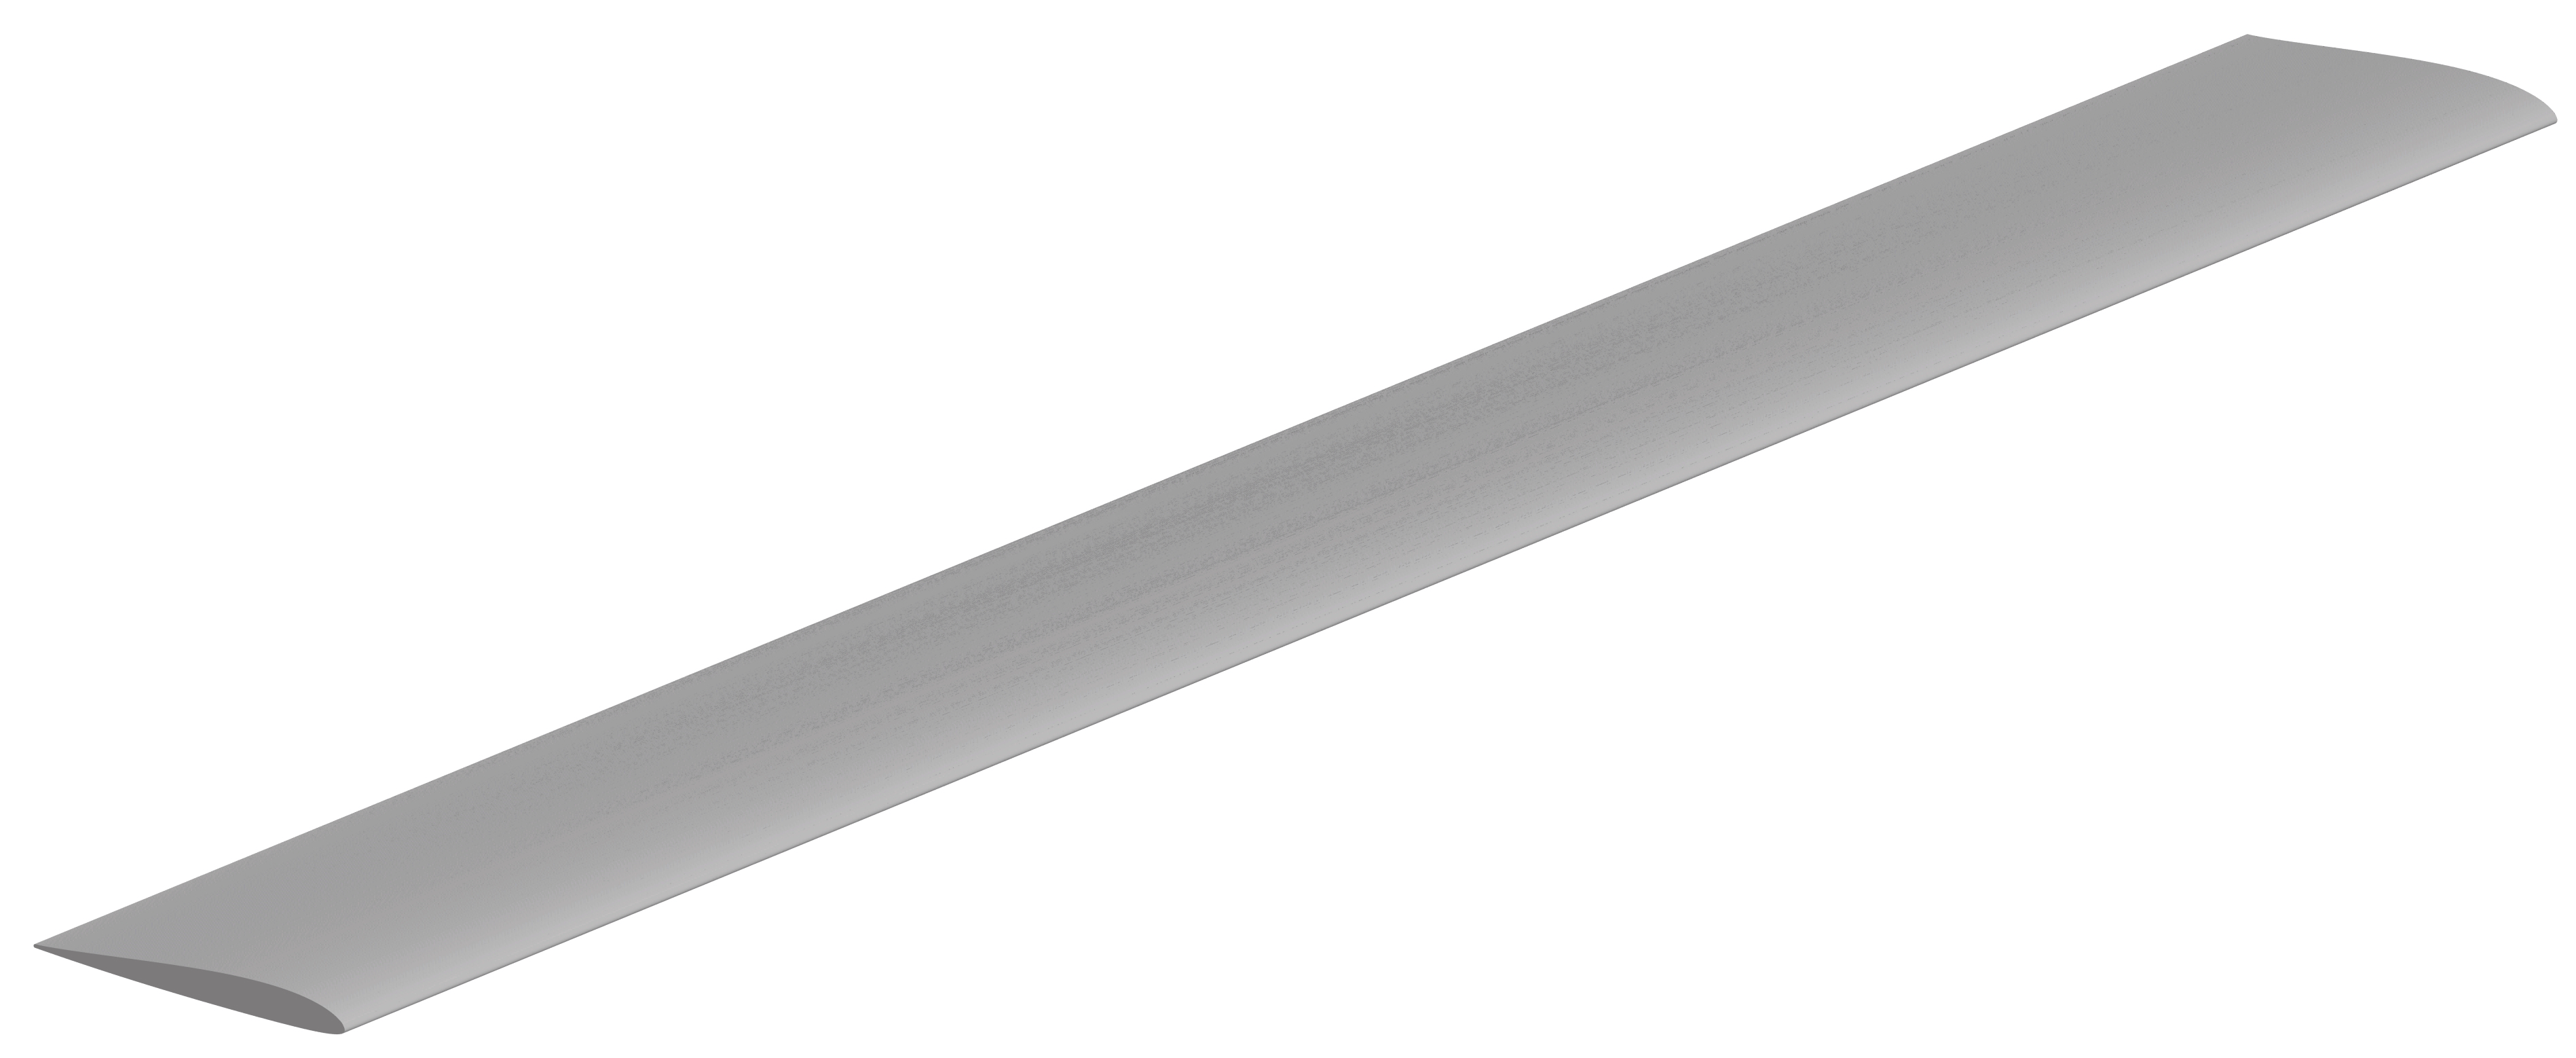
\includegraphics  [ height=6cm] {images/FileImg/rendering.jpg}
\caption{\footnotesize Rendering ala di elevato allungamento con profilo costante PW106. \newline CATIA V5\-6R2017}
\label{fig:catia}
\end{figure}
%   % !TeX program = PdfLaTeX
% !TeX root = ../../Elaborati_Aerodinamica_Bruno_Spoti.tex
\chapter{Aerodinamica non viscosa incomprimibile}
Nel seguente capitolo verranno esposti i risultati ottenuti circa le caratteristiche del profilo in termini di retta di portanza, angolo d’attacco ideale e di portanza nulla e coefficiente di momento focale. Infine verranno graficate le distribuzioni del coefficiente di pressione al variare del $C_l $.
\section{Curve di portanza e momento}
Tramite l’utilizzo di XFOIL è stato possibile ottenere l’andamento della curva di portanza del profilo PW106 e quello del momento aerodinamico in termini di soluzione Euleriana incomprimibile, calcolato rispetto al punto ad un quarto della corda. Al fine di calcolare il centro aerodinamico è stata applicata la formula~\vref{eq:centroAerodinamico}, dalla particolarizzazione della quale è stata ricavata anche la curva del momento rispetto il bordo d'attacco riportate in figura~\vref{fig:cmIncomp}. I principali risultati sono riportati in tabella~\vref{tab:risultatiXFOIL}.


\renewcommand\arraystretch{1.4} 
\begin{table} [!h]\centering \rowcolors{1}{}{grigio_chiaro}
\begin{tabular}{c| c}
\toprule
  &  \emph{XFOIL 6.99} \\ 
\midrule
${\alpha}_{\mathrm{zl}}$ & $-0.872^\circ$ \\
${C_{l_{\alpha}}}$ & $0.117 \, \si{deg}^{-1}$ \\
${ C_{m_{{\alpha}_{c4}}}}$ &$-0.0007 \, \si{deg}^{-1}$  \\ 
${ C_{m_{{\alpha}_{le}}}}$ &$-0.0301 \, \si{deg}^{-1}$\\
 $\frac{X_{ac}}{c}$  & 0.256\\
\bottomrule
\end{tabular}
\caption {Profilo alare PW106, principali risultati ottenuti tramite XFOIL 6.99.}
\label{tab:risultatiXFOIL}
\end{table}

\begin{equation}
\frac {x_{ac}}{c}=\frac {x_{c_4}}{c} - \frac{ C_{m_{{\alpha}_{c4}}}}{C_{l_{\alpha}}}
\label{eq:centroAerodinamico}
\end{equation}


\begin{figure} [H]
\centering
\begin{tikzpicture} 
\begin{axis} [ 
ylabel style={rotate=-90}, xmin=-10, 
xmax=10, 
ymin=-1,
ymax=1.6,
xlabel=$ \alpha$, 
ylabel=$ C_l $,
ytick={-1,-0.8,-0.6,-0.4,-0.2,0,0.2,0.4,0.6,0.8,1,1.2,1.4,1.6},
width=9cm,
height=7.5cm,
scale only axis,
grid=major] 
\addplot [black]
file{images/fileDat/AnalisiNonViscoseIncomprimibili/Cl_vs_alpha.dat};
\end{axis}
\end{tikzpicture}
\caption{\footnotesize Profilo alare PW106, curva di portanza, soluzione euleriana incomprimibile.  XFOIL 6.99 }\label{fig:cl}
\end{figure}
\noindent
\\ 

\begin{figure} [h!]
\centering
\begin{tikzpicture} 
\begin{axis} [ 
ylabel style={rotate=-90}, xmin=-10, 
xmax=10, 
ymin=-0.35,
ymax=0.3,
xlabel=$ \alpha$, 
ylabel=$ C_{m}$,
%ytick={-0.5,-0.4,-0.3,-0.2,-0.1,0,0.1,0.2,0.3,0.4,0.5},
width=9cm,
height=7.5 cm,
scale only axis,
grid=major] 
\addplot [black]
file{images/fileDat/AnalisiNonViscoseIncomprimibili/Cm_c_quarti_vs_alpha_v2.dat};
\addplot [black,dashed]
file{images/fileDat/AnalisiNonViscoseIncomprimibili/Cm_le_vs_alpha_v2.dat};
\addplot [black,dashdotted]
file{images/fileDat/AnalisiNonViscoseIncomprimibili/Cm_ac_vs_alpha_v2.dat};
\legend {${ C_{m_{c4}}}$, ${ C_{m_{le}}}$ , ${ C_{m_{ac}}}$}
\end{axis}
\end{tikzpicture}
\caption{\footnotesize Profilo alare PW106, curve di momento, soluzione euleriana incomprimibile al variare del polo.  XFOIL 6.99 }\label{fig:cmIncomp}
\end{figure}



\noindent \\
\section{Centro di Pressione}

Il centro di pressione é quel punto in cui si puó ritenere applicata la risultante delle forze fluidodinamiche agenti sul profilo.
Per calcolarlo si é ricorsi alla formula~\vref{eq:centroPressione}. \cite{prof:tognaccini}

\begin{equation}
-\frac {x_{cp}}{c}=\frac{ C_{m_{le}}}{C_l}
\label{eq:centroPressione}
\end{equation}

Il $ C_{m_{le}}$ è il coefficiente di momento calcolato rispetto al bordo d’attacco del profilo. \\
Esso può essere ottenuto tramite il calcolo dei coefficienti di Fourier dello sviluppo in serie della derivata della linea media, in accordo con la Teoria del Profilo Sottile, i cui risultati saranno in seguito esposti.

\begin{equation}
\label{eqn:zerouno}
C_{m_{le}}= \frac {{\pi}}{4}(c_2-c_1)- \frac {C_l}{4}
\end{equation}

\begin{figure} [h!]
\centering
\begin{tikzpicture} 
\begin{axis} [ 
ylabel style={rotate=-90}, xmin=-3, 
xmax=2, 
ymin=-0.25,
ymax=0.8,
xlabel=$ {\alpha}$, 
ylabel=$\frac{x_{cp}}{c}$,
width=9cm,
height=7 cm,
scale only axis,
grid=major] 
\addplot [black,smooth]
file{images/fileDat/AnalisiNonViscoseIncomprimibili/XcpCAlpha1.dat};
\addplot [black,smooth]
file{images/fileDat/AnalisiNonViscoseIncomprimibili/XcpCAlpha2.dat};
\end{axis}
\end{tikzpicture}
\caption{\footnotesize Profilo alare PW106, andamento dell'ascissa del centro di pressione al variare di ${\alpha}$.  XFOIL 6.99}\label{fig:cp}
\end{figure}


\section{Risultati della Teoria del Profilo Sottile}

Al fine di calcolare i coefficienti di Fourier dello sviluppo in serie della derivata della linea media, è stato implementato uno script in MATLAB che, ricevendo in ingresso i punti della linea media, consente di ottenere il gradiente della retta di portanza, l’angolo d’attacco ideale e di portanza nulla e il coefficiente di momento di beccheggio rispetto al fuoco.

I coefficienti dello sviluppo in serie di Fourier valgono\\

\begin{equation}
\label{eqn:prima}
c_0= \frac {1}{{\pi}}\int_0^{\pi} C'(x) d{\theta}
\end{equation}

\begin{equation}
\label{eqn:seconda}
c_n= \frac {2}{{\pi}}\int_0^{\pi} C'(x) {\cos}(n{\theta}) d{\theta}
\end{equation}


\noindent \\ \\
Dalle formule \ref{eqn:prima} e \ref{eqn:seconda} sono stati ricavati i seguenti risultati, i cui valori sono riportati in 


\begin {itemize}
\item ${\alpha}_i=c_0$
\item ${\alpha}_{zl}=c_0-\frac {c_1}{2}$
\item $C_{m\frac {c}{4}}=-\frac {{\pi}}{4}(c_1-c_2)$
\end{itemize}

\noindent \\ 
Per il calcolo è stato utilizzato il $C_{l{\alpha}}$ ottenuto con XFOIL pari a $6.73 rad^{-1}$.

%\begin{equation}
%\label{eqn:terza}
%c_{l_{\alpha}}=2{\pi}(1+ k{\tau})
%\end{equation}

%\noindent \\
%Il cui risultato è \\
%
%\begin{center}
% { k=0.79}
%\end {center}


\renewcommand\arraystretch{1.4} 
\begin{table} [!h]\centering \rowcolors{1}{}{grigio_chiaro}
\begin{tabular}{c| c}
\toprule
  &  \emph{Teoria del profilo sottile} \\ 
\midrule
${\alpha}_{i} $ & $0.0363^\circ$ \\
${\alpha}_{\mathrm{zl}}$ & $-0.789^\circ$ \\
${ C_{m_{{\alpha}_{c4}}}}$ &$-0.00103$  \\ 
\bottomrule
\end{tabular}
\caption {Profilo alare PW106, principali risultati ottenuti tramite l'applicazione della teoria del profilo sottile implementata mediante MATLAB R2016b.}
\label{tab:profiloSottile}
\end{table}

\section{Coefficiente di Pressione}

Di seguito sono riportati gli andamenti del coefficiente di pressione del profilo alare in studio, nell’ ipotesi di campo Euleriano incomprimibile, in funzione dell’ascissa adimensionalizzata rispetto la corda a vari $C_l$, anche non piccoli.\\ \\


\begin{figure} [h!]
\centering
\begin{tikzpicture} 
\begin{axis} [ 
ylabel style={rotate=-90}, xmin=0, 
xmax=1, 
ymin=-17,
ymax=2,
xlabel=$\frac{x}{c}$, 
ylabel=$C_p$ ,
 y dir=reverse,
width=12cm,
height=7 cm,
scale only axis,
grid=major] 
\addplot [black]
file{images/fileDat/AnalisiNonViscoseIncomprimibili/cp_-1_Inv_Inc_dorso.dat};
\addplot [black, dashed]
file{images/fileDat/AnalisiNonViscoseIncomprimibili/cp_-1_Inv_Inc_ventre.dat};
\legend {Dorso,Ventre}
\end{axis}
\end{tikzpicture}
\caption{\footnotesize Profilo alare PW106, distribuzione del coefficiente di pressione $C_l=-1 \  ( \alpha=-9.40^\circ$). Soluzione Euleriana incomprimibile.  XFOIL 6.99 }\label{fig:cp}
\end{figure}

\begin{figure} 
\centering
\begin{tikzpicture} 
\begin{axis} [ 
ylabel style={rotate=-90}, xmin=0, 
xmax=1, 
ymin=-1.5,
ymax=1,
xlabel=$\frac{x}{c}$, 
ylabel=$C_p$ ,
 y dir=reverse,
width=12cm,
height=7 cm,
scale only axis,
grid=major] 
\addplot [black]
file{images/fileDat/AnalisiNonViscoseIncomprimibili/cp_0_Inv_Inc_dorso.dat};
\addplot [black, dashed]
file{images/fileDat/AnalisiNonViscoseIncomprimibili/cp_0_Inv_Inc_ventre.dat};
\legend {Dorso,Ventre}
\end{axis}
\end{tikzpicture}
\caption{\footnotesize Profilo alare PW106, distribuzione del coefficiente di pressione $C_l=0 \ ( \alpha \!= \! -0.873^\circ$). Soluzione Euleriana incomprimibile.  XFOIL 6.99 }\label{fig:cp}
\end{figure}


\begin{figure} 
\centering
\begin{tikzpicture} 
\begin{axis} [ 
ylabel style={rotate=-90}, xmin=0, 
xmax=1, 
ymin=-1.2,
ymax=1,
xlabel=$\frac{x}{c}$, 
ylabel=$C_p$ ,
 y dir=reverse,
width=12cm,
height=7 cm,
scale only axis,
grid=major] 
\addplot [black]
file{images/fileDat/AnalisiNonViscoseIncomprimibili/cp_0.5_Inv_Inc_dorso.dat};
\addplot [black, dashed]
file{images/fileDat/AnalisiNonViscoseIncomprimibili/cp_0.5_Inv_Inc_ventre.dat};
\legend {Dorso,Ventre}
\end{axis}
\end{tikzpicture}
\caption{\footnotesize Profilo alare PW106, distribuzione del coefficiente di pressione $C_l=0.5 \ ( \alpha=3.39^\circ )$. Soluzione Euleriana incomprimibile.  XFOIL 6.99 }\label{fig:cp}
\end{figure}
\noindent \\


\begin{figure} 
\centering
\begin{tikzpicture} 
\begin{axis} [ 
ylabel style={rotate=-90}, xmin=0, 
xmax=1, 
ymin=-3.5,
ymax=1.5,
xlabel=$\frac{x}{c}$, 
ylabel=$C_p$ ,
 y dir=reverse,
width=12cm,
height=7 cm,
scale only axis,
grid=major] 
\addplot [black]
file{images/fileDat/AnalisiNonViscoseIncomprimibili/cp_1_Inv_Inc_dorso.dat};
\addplot [black, dashed]
file{images/fileDat/AnalisiNonViscoseIncomprimibili/cp_1_Inv_Inc_ventre.dat};
\legend {Dorso,Ventre}
\end{axis}
\end{tikzpicture}
\caption{\footnotesize Profilo alare PW106, distribuzione del coefficiente di pressione $C_l=1 \ ( \alpha=7.68^\circ$). Soluzione Euleriana incomprimibile.  XFOIL 6.99 }\label{fig:cp}
\end{figure}
\noindent \\


\begin{figure} 
\centering
\begin{tikzpicture} 
\begin{axis} [ 
ylabel style={rotate=-90}, xmin=0, 
xmax=1, 
ymin=-9,
ymax=1.5,
xlabel=$\frac{x}{c}$, 
ylabel=$C_p$ ,
 y dir=reverse,
width=12cm,
height=7 cm,
scale only axis,
grid=major] 
\addplot [black]
file{images/fileDat/AnalisiNonViscoseIncomprimibili/cp_1.4_Inv_Inc_dorso.dat};
\addplot [black, dashed]
file{images/fileDat/AnalisiNonViscoseIncomprimibili/cp_1.4_Inv_Inc_ventre.dat};
\legend {Dorso,Ventre}
\end{axis}
\end{tikzpicture}
\caption{\footnotesize Profilo alare PW106, distribuzione del coefficiente di pressione $C_l=1.4 \ ( \alpha=10.3^\circ$). Soluzione Euleriana incomprimibile.  XFOIL 6.99 }\label{fig:cp}
\end{figure}
\noindent 





%   % !TeX program = PdfLaTeX
% !TeX root = ../../Elaborati_Aerodinamica_Bruno_Spoti.tex
\chapter{Effetti della Comprimibilità}

Lo studio del profilo alare PW106 fin ora condotto si è basato sul modello di moto incomprimibile, valido esclusivamente alle basse velocità. Gli effetti dell’aumento del numero di Mach possono ancora essere studiati in un campo lineare se è valida l’ipotesi di piccole perturbazioni.\\
Nel presente capitolo si terranno in conto gli effetti della comprimibilità in campo subsonico lineare andando preliminarmente a calcolare il numero di Mach critico inferiore e valutandone la variabilità con il $C_l$. Successivamente si analizzeranno gli effetti dell'aumento del numero di Mach sul $C_{p}$ in campo subsonico.
Infine saranno confrontati i risultati ottenuti con XFOIL con quelli ricavati con le regole di similitudine di Prandtl-Glauert per il moto subsonico comprimibile.

\noindent \\
\section{Numero di Mach Critico Inferiore}


Al fine di poter calcolare il numero di Mach Critico Inferiore, tramite MATLAB  sono stati costruiti alcuni rami del Abbaco che esprime il $Cp_{min}$ in funzione di $M_{\infty}$ e sul quale vi è la curva del $Cp^{*}$. \\ Dall’intersezione di queste due curve, per un certo angolo d’attacco, si ottiene la valutazione del numero di Mach Critico Inferiore ( $M_{\infty crit}$).\\ 

L’angolo per il quale è stato calcolato il $M_{\infty crit}$ è  ${\alpha}=2^\circ$.\\

Con XFOIL sono stati ricavati i valori del $Cp_{min}$ per vari valori del numero di Mach e i valori del $Cp^*$, ossia il $C_p$ del campo di moto ove si raggiungono condizioni soniche.


\begin{figure} 
\centering
\begin{tikzpicture} 
\begin{axis} [ 
 xmin=0, 
xmax=1, 
ymin=-16,
ymax=0,
xlabel=$M_{\infty}$, 
ylabel=$Cp_{min}$ ,
 y dir=reverse,
width=12cm,
height=7cm,
scale only axis,
grid=major] 
\addplot [black,very thick,smooth,dashed]
file{images/fileDat/Comprimibilità/m_cp_star.dat};
\addplot [black,smooth]
file{images/fileDat/Comprimibilità/cPIncMin_atCl_-0.9.dat};
\addplot [black,smooth]
file{images/fileDat/Comprimibilità/cPIncMin_atCl_-0.7.dat};
\addplot [black,smooth]
file{images/fileDat/Comprimibilità/cPIncMin_atCl_-0.5.dat};
\addplot [black,smooth]
file{images/fileDat/Comprimibilità/cPIncMin_atCl_-0.3.dat};
\addplot [black,smooth]
file{images/fileDat/Comprimibilità/cPIncMin_atCl_-0.1.dat};
\addplot [black,smooth]
file{images/fileDat/Comprimibilità/cPIncMin_atCl_0.11.dat};
\addplot [black,smooth]
file{images/fileDat/Comprimibilità/cPIncMin_atCl_0.3.dat};
\addplot [black,smooth]
file{images/fileDat/Comprimibilità/cPIncMin_atCl_0.5.dat};
\addplot [black,smooth]
file{images/fileDat/Comprimibilità/cPIncMin_atCl_0.7.dat};
\addplot [black,smooth]
file{images/fileDat/Comprimibilità/cPIncMin_atCl_0.9.dat};
\legend {$Cp^*$,$Cp_{min}$}
\end{axis}
\end{tikzpicture}
\caption{\footnotesize Abbaco per il calcolo del numero di Mach Critico Inferiore. Curve del $Cp_{min}$ parametrizzatere per $C_l$ che varia tra -0.9 e 0.9 con passo 0.2. Matlab R2016b. XFOIL~6.99 }\label{fig:cp}
\end{figure}
\noindent 

Tramite MATLAB è stato calcolato il punto di intersezione tra le due curve al fine di calcolare il valore del numero di Mach richiesto:

\begin{center}
\bfseries  {$ M_{\infty crit}({\alpha}=2^\circ)$=0.624}
\end {center}

È interessante valutare l’andamento del $ M_{\infty crit} $ al variare del $C_l$. Ció è stato fatto tramite l’Abbaco introdotto entrando in tal grafico con il valore del $Cp_{min}$ ottenuto da XFOIL per diversi $C_l$.\\
Il massimo valore trovato di  $ M_{\infty crit} $ è 0.727, ad un Coefficiente di Portanza di 0.11, come si evince dalla figura~\vref{fig:mcrCL}
\begin{figure} [h!]
\centering
\begin{tikzpicture} 
\begin{axis} [ 
xmin=0, 
xmax=1, 
ymin=-1,
ymax=1,
ylabel=$C_l$, 
xlabel=$ M_{\infty crit} $,
ylabel style={rotate=-90},
width=10cm,
height=6 cm,
scale only axis,
grid=major] 
\addplot [black,mark=*,mark options={solid}]
file{images/fileDat/Comprimibilità/grafico_cl_mcrinf.dat};
\end{axis}
\end{tikzpicture}
\caption{\footnotesize Profilo alare PW106, $M_{\infty crit} $  al variare del coefficiente di portanza. Matlab R2016b. XFOIL~6.99}\label{fig:mcrCL}
\end{figure}
\noindent \\

\section{Effetti della comprimibilità }



In primo luogo è interessante valutare come varia la distribuzione del Coefficiente di Pressione sul profilo.

\noindent \\

\begin{figure} [h!]
\centering
\begin{tikzpicture} 
\begin{axis} [ 
ylabel style={rotate=-90}, xmin=0, 
xmax=1, 
ymin=-1.5,
ymax=1.5,
xlabel=$\frac{x}{c}$, 
ylabel=$C_p$ ,
 y dir=reverse,
width=12cm,
height=7 cm,
scale only axis,
grid=major] 
\addplot [black,dashed]
file{images/fileDat/Comprimibilità/cp_alfa2_M0.624.dat};
\addplot [black]
file{images/fileDat/Comprimibilità/cp_a2_M0.dat};
\legend {$M=0.624$,$M=0$}
\end{axis}
\end{tikzpicture}
\caption{\footnotesize Profilo alare PW106, confronto del Coefficiente di Pressione per il campo incomprimibile e comprimibile subsonico per $\alpha=2^\circ$. XFOIL 6.69}\label{fig:cp}
\end{figure}

\noindent   \\

Per effetto della comprimibilità cambierà la distribuzione del Coefficiente di pressione lungo il profilo. In particolare, all’aumentare del numero di Mach, le zone espanse espandono di più, e quelle compresse comprimono di più.\\ Nel grafico esistono alcuni punti, detti “Punti Neutri” che godono dell’invarianza del Cp, al variare del numero di Mach. Questi sono i punti per i quali il Coefficiente di pressione vale zero.\\ 

Tramite XFOIL è possibile valutare l’andamento del $C_l$ all’aumentare del numero di Mach a monte (vedi figura~\vref{fig:cp1.4}). % È stato considerato come punto di partenza per M=0 un $C_l =0.67$. Questo coefficiente di portanza è relativo, in campo incomprimibile, ad un angolo d’attacco $ \alpha =2^\circ$ e ad esso corrisponde un numero di Mach Critico Inferiore di 0.624.\\  
Dal grafico ottenuto si nota chel $C_l$ cresce all’aumentare del un $M_{\infty}$.


\begin{figure} [h!]
\centering
\begin{tikzpicture} 
\begin{axis} [ 
legend style={at={(0.98,0.25)}},
ylabel style={rotate=-90}, xmin=-4, 
xmax=9, 
ymin=-0.5,
ymax=1.8,
xlabel=$\alpha$,
ylabel=$C_l$, 
width=10cm,
height=12 cm,
scale only axis,
grid=major] 
\addplot [black,smooth]
file{images/fileDat/Comprimibilità/curva_portanza_M0.dat};
\addplot [black,smooth,dashed]
file{images/fileDat/Comprimibilità/curva_portanza_M0_2.dat};
\addplot [black,smooth,dashdotted]
file{images/fileDat/Comprimibilità/curva_portanza_M0_4.dat};
\addplot [black,smooth,dotted]
file{images/fileDat/Comprimibilità/curva_portanza_M0_6.dat};
\legend {$M=0$,$M=0.2$, $M=0.4$,$M=0.6$}
\end{axis}
\end{tikzpicture}
\caption{\footnotesize Profilo alare PW106, andamento della curva di portanza al variare del $M_{\infty}$ . XFOIL 6.99}\label{fig:cp1.4}
\end{figure}

\begin{figure} [h!]
\centering
\begin{tikzpicture} 
\begin{axis} [ 
ylabel style={rotate=-90}, xmin=0, 
xmax=0.7, 
ymin=0.3,
ymax=0.5,
xlabel=$M_{\infty}$,
ylabel=$C_l$, 
width=10cm,
height=6 cm,
scale only axis,
grid=major] 
\addplot [black,smooth]
file{images/fileDat/Comprimibilità/cl_mach.dat};
\end{axis}
\end{tikzpicture}
\caption{\footnotesize Profilo alare PW106, andamento del $C_l $  al variare del $M_{\infty}$ per $ \alpha =2^\circ$ . XFOIL 6.99}\label{fig:cp1.4}
\end{figure}


\noindent \\ \\ 

\section{Similitudine di Prandtl-Glauert }

Con la similitudine di Prandtl-Glauert è possibile studiare campi comprimibile subsonici attraverso teorie incomprimibili. Ciò è fatto attraverso un cambiamento di variabili che ci consente di scrivere le seguenti equazioni 

\begin{equation}
\label{eqn:prandtcll}
[C_l]_{M,{\alpha},{\tau},{\gamma}}=\frac {1}{\sqrt{1-M^2_{\infty}}}[C_l]_{M=0,{\alpha},{\tau},{\gamma}}
\end{equation}


\begin{equation}
\label{eqn:prandtl}
[C_p]_{M,{\alpha},{\tau},{\gamma}}=\frac {1}{\sqrt{1-M^2_{\infty}}}[C_p]_{M=0,{\alpha},{\tau},{\gamma}}
\end{equation}


Il codice XFOIL, per la risoluzione dei campi comprimibili, ricorre alla similitudine di Karman e Tsein che vanta una migliore accuratezza in alto subsonico rispetto la regola di Prandtl-Glauert. \\
Di seguito si mostra un confronto tra la risoluzione del campo di moto comprimibile con i due approcci citati in termini di $C_l$ e Cp. \\


Viene fissato un $C_l=0.3373$ cui corrisponde un $ M_{\infty crit}=0.624$. Da questo valore di partenza ($C_l=0.3373$, $M_{\infty}=0$), attraverso l'utilizzo di un codice MATLAB, si calcolano i valori del $C_l$ al variare del $ M_{\infty}$ con la similitudine Prandtl-Glauert fino ad un valore di $M_{\infty}=0.624$.\\ Il grafico ricavato viene confrontato con quello ottenuto da XFOIL.

\begin{figure} [H]
\centering
\begin{tikzpicture} 
\begin{axis} [ 
ylabel style={rotate=-90}, xmin=0, 
xmax=0.7, 
ymin=0.3,
ymax=0.55,
ylabel=$C_l$, 
xlabel=$M_{\infty}$ ,
width=10cm,
height=6 cm,
scale only axis,
grid=major] 
\addplot [black,very thick,dashed]
file{images/fileDat/Comprimibilità/cl_mach.dat};
\addplot [black,very thick]
file{images/fileDat/Comprimibilità/prandtl.dat};
\legend {XFOIL,Similitudine Prandtl-Glauert}
\end{axis}
\end{tikzpicture}
\caption{\footnotesize Profilo alare PW106, confronto del Coefficiente di portanza per il campo comprimibile subsonico calcolato con la similitudine di Prandtl-Glauert e con XFOIL per $C_l=0.34$ a $ M_{\infty}=0$ ($ M_{\infty crit}=0.624)$. XFOIL 6.99. Matlab R2016b}\label{fig:cp}
\end{figure}

Per valutare la distribuzione del coefficiente di pressione in campo comprimibile utilizzando la similitudine di  Karman-Tsein è stato ricavato il Cp per $C_l=0.34$ e $M_{\infty}=0.624$ tramite XFOIL, mentre per ottenere il  $C_p$ con la similitudine di Prandtl-Glauert è stato implementato uno script in MATLAB che, a partire dai valori del $C_p$ per $C_l=0.34$ e $M_{\infty}=0$ ottenuti con XFOIL, calcola la distribuzione del coefficiente di pressione che tiene conto degli effetti della comprimibilità.

\begin{figure} [H]
\centering
\begin{tikzpicture} 
\begin{axis} [ 
ylabel style={rotate=-90}, xmin=0, 
xmax=1, 
ymin=-1.5,
ymax=1.5,
xlabel=$\frac{x}{c}$, 
ylabel=$C_p$ ,
 y dir=reverse,
width=12cm,
height=6 cm,
scale only axis,
grid=major] 
\addplot [black,very thick,dashed]
file{images/fileDat/Comprimibilità/cp_alfa2_M0.624.dat};
\addplot [black,very thick]
file{images/fileDat/Comprimibilità/cpprandtl.dat};
\legend {XFOIL,Similitudine Prandtl-Glauert}
\end{axis}
\end{tikzpicture}
\caption{\footnotesize Profilo alare PW106, confronto del coefficiente di pressione per il campo comprimibile subsonico calcolato con la similitudine di Prandtl-Glauert e con XFOIL per $C_l=0.34$ e $M_{\infty}=0.624$. XFOIL 6.99. Matlab R2016b}\label{fig:cp}
\end{figure}

%   % !TeX program = PdfLaTeX
% !TeX root = ../../Elaborati_Aerodinamica_Bruno_Spoti.tex
\chapter{Effetti viscosi}

In questo capitolo sarà studiata l’aerodinamica del profilo alare  PW106 ad assetti piccoli e medi, tenendo conto degli effetti viscosi. \\ A tal proposito in primo luogo saranno esaminati gli effetti della variazione del numero di Reynolds sulle curve di portanza e sulla polare, analizzandone alcuni casi più significativi, al fine di evidenziare l’effetto che ha la variazione di tale valore adimensionale sulle prestazioni del profilo. Verrà, inoltre, analizzata la variazione del coefficiente di pressione dovuta agli effetti di scala. Saranno, poi, presi in considerazione i più significativi parametri di strato limite e saranno analizzati gli effetti della transizione forzata, fissata ad un certo valore della corda, e quelli che il parametro $n_{cr}$, che tiene conto degli effetti di turbolenza e rugosità, sull’aerodinamica del profilo.\\
Tali analisi saranno condotte mediante l’ausilio di XFOIL. 

\section{Curva di Portanza e polare}

Il profilo analizzato è un profilo progettato per lavorare a bassi numeri di Reynolds. Nella curva di Portanza ottenuta con XFOIL, tuttavia, anche a $Re$ più elevati, non si riscontrano particolari oscillazioni, pertanto sono stati scelti i seguenti valori: \\

\begin {itemize}
\item $Re=5\times10^5  $ ${\to}$ $ {\alpha}_\mathrm{stall}=13^\circ$  ${\to}$ $C_{l_\mathrm{max}}=1.28$;
\item $Re=1\times10^6$ ${\to}$ $ {\alpha}_\mathrm{stall}=13^\circ$  ${\to}$ $C_{l_\mathrm{max}}=1.38$;
\item $Re=3\times10^6$ ${\to}$ $ {\alpha}_\mathrm{stall}=16^\circ$  ${\to}$ $C_{l_\mathrm{max}}=1.56$;
\item $Re=1\times10^7$ ${\to}$ $ {\alpha}_\mathrm{stall}=18^\circ$  ${\to}$ $C_{l_\mathrm{max}}=1.76$.
\end{itemize}

\noindent \\
Dall'osservazione dei grafici riportati nelle figure \ref{fig:cla11} e \ref{fig:pol} si notano alcuni degli effetti che ha l’incremento del numero di Reynolds sulle prestazioni del profilo. Al crescere di $Re$, la curva di portanza aumenta il suo tratto lineare, il che vuol dire che aumenta il $C_{l_\mathrm{max}}$ e, conseguentemente, l’angolo di stallo. Dalle polari del profilo si nota la progressiva diminuzione del $C_{d_\mathrm{min}}$ al crescere del numero di Reynolds connesso al già citato aumento del $C_{l_\mathrm{max}}$.

\begin{figure} [H]
\centering
\begin{tikzpicture} 
\begin{axis} [ 
legend style={at={(0.3,0.98)}},
ylabel style={rotate=-90}, xmin=-20, 
xmax=25, 
ymin=-2,
ymax=2,
xlabel=${\alpha}$,
ylabel=$C_l$ ,
width=12cm,
height=19 cm,
scale only axis,
grid=major] 
\addplot [black, smooth,mark=*]
file{images/fileDat/EffettiViscosi/Cl_vs_alpha_Re_5_10_5.dat};
\addplot [black,smooth,mark=square]
file{images/fileDat/EffettiViscosi/Cl_vs_alpha_Re_1_10_6.dat};
\addplot [black, smooth,mark=diamond*]
file{images/fileDat/EffettiViscosi/Cl_vs_alpha_Re_3_10_6.dat};
\addplot [black, smooth,mark=star]
file{images/fileDat/EffettiViscosi/Cl_vs_alpha_Re_1_10_7.dat};
\legend {$Re=5\times10^5  $,$Re=1\times10^6$,$Re=3\times10^6$,$Re=1\times10^7$}
\end{axis}
\end{tikzpicture} 
\caption{\footnotesize Profilo alare PW106, confronto delle curve di portanza al variare del numero di Reynolds. XFOIL 6.99 }
\label{fig:cla11}
\end{figure}

\begin{figure} [H]
\centering
\begin{tikzpicture} 
\begin{axis} [ 
legend style={at={(0.98,0.30)}},
ylabel style={rotate=-90}, xmin=0, 
ymin=-2,
ymax=2.2,
xlabel=$C_d$ (drag count),
ylabel=$C_l$ ,
width=11cm,
height=11cm,
scale only axis,
grid=major] 
\addplot [black, smooth,mark=*]
file{images/fileDat/EffettiViscosi/cd_cl_5_10_5.dat};
\addplot [black,smooth,mark=square]
file{images/fileDat/EffettiViscosi/cd_cl_10_6.dat};
\addplot [black, smooth,mark=diamond*]
file{images/fileDat/EffettiViscosi/cd_cl_3_10_6.dat};
\addplot [black, smooth,mark=star]
file{images/fileDat/EffettiViscosi/cd_cl_10_7.dat};
\legend {$Re=5\times10^5  $,$Re=1\times10^6$,$Re=3\times10^6$,$Re=1\times10^7$}
\end{axis}
\end{tikzpicture}
\caption{\footnotesize Profilo alare PW106, confronto delle polari al variare del numero di Reynolds. XFOIL 6.99 }
\label{fig:pol}
\end{figure}

\begin{figure} [H]
\centering
\begin{tikzpicture} 
\begin{axis} [ 
legend style={at={(0.98,0.90)}},
ylabel style={rotate=-90}, xmin=0, 
xmax=250, 
ymin=-1,
ymax=1,
xlabel=$C_d$ (drag count),
ylabel=$C_l$ ,
width=9cm,
height=6cm,
scale only axis,
grid=major] 
\addplot [black, smooth,mark=*]
file{images/fileDat/EffettiViscosi/cd_cl_5_10_5.dat};
\addplot [black,smooth,mark=square]
file{images/fileDat/EffettiViscosi/cd_cl_10_6.dat};
\addplot [black, smooth,mark=diamond*]
file{images/fileDat/EffettiViscosi/cd_cl_3_10_6.dat};
\addplot [black, smooth,mark=star]
file{images/fileDat/EffettiViscosi/cd_cl_10_7.dat};
\legend {$Re=5\times10^5 $,$Re=1\times10^6$,$Re=3\times10^6$,$Re=1\times10^7$}
\end{axis}
\end{tikzpicture}
\caption{\footnotesize Polari del profilo PW106 al variare del numero di Reynolds, zoom della zona di alta e media velocità. XFOIL 6.99 }
\label{fig:pol}
\end{figure}


\section{Coefficiente di pressione al variare del numero di Reynolds }

\noindent \\ 

Di seguito sono confrontati i grafici del $C_p$ ad un certo angolo d’attacco del profilo e fissato $n_{cr}$, per vari numeri di Reynolds così da vedere la formazione e l’evoluzione delle bolle laminari in dipendenza dal Re. Successivamente si vedrà l’effetto della variazione di ${\alpha}$  ad un fissato numero di Reynolds. \\
Gli sviluppi applicativi, in questo capitolo, saranno fatti in condizioni di piccoli e medi angoli d'attacco, rimandando al successivo capitolo lo studio dell'alta portanza.\\
Preliminarmente, al fine di comprendere le differenze tra la soluzione Euleriana e quella viscosa, sarà graficato l'andamento del $C_p$ per il profilo PW106 ad un fissato angolo d’attacco, in assenza di effetti viscosi, e con un $Re=2.5\times10^5$.\\


\begin{figure} [H]
\centering
\begin{tikzpicture} 
\begin{axis} [ 
ylabel style={rotate=-90}, xmin=0, 
xmax=1, 
ymin=-2,
ymax=1,
xlabel=$\frac{x}{c}$, 
ylabel=$C_p$ ,
 y dir=reverse,
width=12cm,
height=6 cm,
scale only axis,
grid=major] 
\addplot [black,thin]
file{images/fileDat/EffettiViscosi/Cp_alfa_3_Invdorso.dat};
\addplot [black,thin,dashed]
file{images/fileDat/EffettiViscosi/Cp_alfa_3_Invventre.dat};
\addplot [black,ultra thick]
file{images/fileDat/EffettiViscosi/Cp_alfa_3_Re_2.5_10e5dorso.dat};
\addplot [black,ultra thick,dashed]
file{images/fileDat/EffettiViscosi/Cp_alfa_3_Re_2.5_10e5ventre.dat};
\draw[rotate=-2] (0.44, -0.5) ellipse (0.15 and 0.3);
\legend {Soluzione Euleriana dorso, Soluzione Euleriana ventre, Soluzione viscosa  dorso $Re=2.5\times10^5$, Soluzione viscosa ventre$Re=2.5\times10^5$}
\end{axis}
\end{tikzpicture}
\caption{\footnotesize Profilo PW106, confronto del coefficiente di pressione $ \alpha=3^\circ$. Soluzione Euleriana ed effetti viscosi. XFOIL 6.99}\label{fig:cpre}
\end{figure}
\noindent  \\

Dalla figura \ref{fig:cpre} si nota una sostanziale differenza tra la distribuzione del $C_p$ Euleriano e quello ottenuto considerando gli effetti della viscosità. In quest'ultimo si nota un {\itshape plateau} di pressione, ossia una zona ove il $C_p$ non aumenta né diminuisce. Questo fenomeno è dovuto alla presenza di una {\itshape bolla laminare}, cioè una zona ove il flusso separa laminare e riattacca turbolento. La bolla laminare individua una parte del campo (sotto) ove il flusso è reverso e una (sopra) ove il flusso è diretto. Il fenomeno della bolla laminare si presenta in maniera più evidente a bassi numeri di Reynolds, pertanto per le successive applicazioni lavoreremo a $Re$ non elevati.

\begin{figure} [H]
\centering
\begin{tikzpicture} 
\begin{axis} [ 
ylabel style={rotate=-90}, xmin=0, 
xmax=1, 
ymin=-1,
ymax=1,
xlabel=$\frac{x}{c}$, 
ylabel=$C_p$ ,
 y dir=reverse,
width=12cm,
height=7 cm,
scale only axis,
grid=major] 
\addplot [black,very thin]
file{images/fileDat/EffettiViscosi/Cp_alfa_0_Re_2.5_10e5dorso.dat};
\addplot [black,semithick]
file{images/fileDat/EffettiViscosi/Cp_alfa_0_Re_5_10e5dorso.dat};
\addplot [black,ultra thick]
file{images/fileDat/EffettiViscosi/Cp_alfa_0_Re_1_10e6dorso.dat};
\addplot [black,very thin, dashed]
file{images/fileDat/EffettiViscosi/Cp_alfa_0_Re_2.5_10e5ventre.dat};
\addplot [black,semithick, dashed]
file{images/fileDat/EffettiViscosi/Cp_alfa_0_Re_5_10e5ventre.dat};
\addplot [black,ultra thick, dashed]
file{images/fileDat/EffettiViscosi/Cp_alfa_0_Re_1_10e6ventre.dat};
\draw[rotate=-2] (0.6, -0.2) ellipse (0.15 and 0.3);
\legend {$Re=2.5\times10^5$,$Re=5\times10^5  $,$Re=1\times10^6$}
\end{axis}
\end{tikzpicture}
\caption{\footnotesize Profilo alare PW106, confronto del coefficiente di pressione $ \alpha=0^\circ$ sul dorso del profilo (linea continua) e sul ventre (linea tratteggiata) al variare del numero di Reynolds. XFOIL 6.99}\label{fig:cpre1}
\end{figure}
\noindent \\ \\ 

\begin{figure} [H]
\centering
\begin{tikzpicture} 
\begin{axis} [ 
ylabel style={rotate=-90}, xmin=0, 
xmax=1, 
ymin=-1,
ymax=1,
xlabel=$\frac{x}{c}$, 
ylabel=$C_p$ ,
 y dir=reverse,
width=12cm,
height=7 cm,
scale only axis,
grid=major] 
\addplot [black,very thin]
file{images/fileDat/EffettiViscosi/Cp_alfa_2_Re_2.5_10e5dorso.dat};
\addplot [black,semithick]
file{images/fileDat/EffettiViscosi/Cp_alfa_2_Re_5_10e5dorso.dat};
\addplot [black,ultra thick]
file{images/fileDat/EffettiViscosi/Cp_alfa_2_Re_1_10e6dorso.dat};
\addplot [black,very thin, dashed]
file{images/fileDat/EffettiViscosi/Cp_alfa_2_Re_2.5_10e5ventre.dat};
\addplot [black,semithick, dashed]
file{images/fileDat/EffettiViscosi/Cp_alfa_2_Re_5_10e5ventre.dat};
\addplot [black,ultra thick, dashed]
file{images/fileDat/EffettiViscosi/Cp_alfa_2_Re_1_10e6ventre.dat};
\draw[rotate=-7] (0.51, -0.54) ellipse (0.15 and 0.23);
\legend {$Re=2.5\times10^5$,$Re=5\times10^5  $,$Re=1\times10^6$,$Re=2.5\times10^5$}
\end{axis}
\end{tikzpicture}
\caption{\footnotesize Profilo alare PW106, confronto del coefficiente di pressione $ \alpha=2^\circ$ sul dorso del profilo (linea continua) e sul ventre (linea tratteggiata) al variare del numero di Reynolds. XFOIL 6.99}\label{fig:cpre2}
\end{figure}
\noindent 

\begin{figure} [H]
\centering
\begin{tikzpicture} 
\begin{axis} [ 
ylabel style={rotate=-90}, xmin=0, 
xmax=1, 
ymin=-1.5,
ymax=1,
xlabel=$\frac{x}{c}$, 
ylabel=$C_p$ ,
 y dir=reverse,
width=12cm,
height=7 cm,
scale only axis,
grid=major] 
\addplot [black,very thin]
file{images/fileDat/EffettiViscosi/Cp_alfa_4_Re_2.5_10e5dorso.dat};
\addplot [black,semithick]
file{images/fileDat/EffettiViscosi/Cp_alfa_4_Re_5_10e5dorso.dat};
\addplot [black,ultra thick]
file{images/fileDat/EffettiViscosi/Cp_alfa_4_Re_1_10e6dorso.dat};
\addplot [black,very thin, dashed]
file{images/fileDat/EffettiViscosi/Cp_alfa_4_Re_2.5_10e5ventre.dat};
\addplot [black,semithick, dashed]
file{images/fileDat/EffettiViscosi/Cp_alfa_4_Re_5_10e5ventre.dat};
\addplot [black,ultra thick, dashed]
file{images/fileDat/EffettiViscosi/Cp_alfa_4_Re_1_10e6ventre.dat};
\draw[rotate=-9] (0.38, -0.8) ellipse (0.15 and 0.3);
\legend {,$Re=2.5\times10^5$,$Re=5\times10^5  $,$Re=1\times10^6$}
\end{axis}
\end{tikzpicture}
\caption{\footnotesize Profilo alare PW106, confronto del coefficiente di pressione $ \alpha=4^\circ$  sul dorso del profilo (linea continua) e sul ventre (linea tratteggiata) al variare del numero di Reynolds. XFOIL 6.99}\label{fig:cpre3}
\end{figure}
\noindent 


Man mano che diminuisce il numero di Reynolds la bolla si allunga e si sposta verso il bordo d'uscita, mentre all'aumentare dell'angolo di attacco, la bolla si sposta verso il LE.\\ Per vedere ciò al variare di $\alpha$ si guardi il seguente grafico, fatto per un numero di Reynolds non troppo alto per visualizzare meglio la presenza delle bolle.

\begin{figure} [H]
\centering
\begin{tikzpicture} 
\begin{axis} [ 
ylabel style={rotate=-90}, xmin=0, 
xmax=1, 
ymin=-1.5,
ymax=1,
xlabel=$\frac{x}{c}$, 
ylabel=$C_p$ ,
 y dir=reverse,
width=12cm,
height=7 cm,
scale only axis,
grid=major] 
\addplot [black,very thin]
file{images/fileDat/EffettiViscosi/Cp_alfa_0_Re_2.5_10e5dorso.dat};
\addplot [black,semithick]
file{images/fileDat/EffettiViscosi/Cp_alfa_2_Re_2.5_10e5dorso.dat};
\addplot [black,ultra thick]
file{images/fileDat/EffettiViscosi/Cp_alfa_4_Re_2.5_10e5dorso.dat};
\addplot [black,very thin, dashed]
file{images/fileDat/EffettiViscosi/Cp_alfa_0_Re_2.5_10e5ventre.dat};
\addplot [black,semithick, dashed]
file{images/fileDat/EffettiViscosi/Cp_alfa_2_Re_2.5_10e5ventre.dat};
\addplot [black,ultra thick, dashed]
file{images/fileDat/EffettiViscosi/Cp_alfa_4_Re_2.5_10e5ventre.dat};
\legend {$\alpha=0^\circ $,$\alpha = 2^\circ$,$ \alpha=4^\circ$}
\end{axis}
\end{tikzpicture}
\caption{\footnotesize Profilo PW106, confronto del Coefficiente di Pressione al variare dell'angolo d'attacco sul dorso del profilo (linea continua) e sul ventre (linea tratteggiata), $Re= 2.5\times10^5$. XFOIL 6.99}\label{fig:cpre4}
\end{figure}
\noindent 

\section{Sviluppo e parametri di Strato Limite}

\noindent \\


Gli effetti viscosi dell'aerodinamica applicata possono essere ritenuti confinati all'interno di una sottile zona in prossimità del corpo, detta \emph{strato limite}, pertanto è sicuramente interessante vedere come cambia lo sviluppo dello strato limite all'aumentare dell'angolo d'attacco e come variano i parametri di strato limite al variare del numero di Reynolds e dell'angolo d'attacco, limitandoci sempre all'analisi di piccoli e medi assetti.\\
\begin{figure}[H]
\centering
\subfloat[][$\alpha=0^\circ$]
{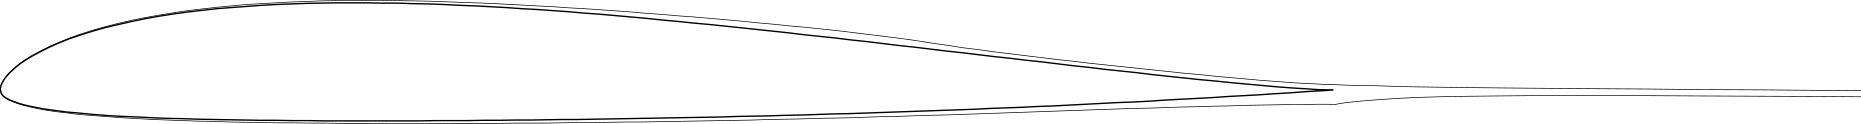
\includegraphics[width=.95\textwidth]{images/fileImg/alfa0_Re_25e4.png}} \\
\subfloat[][$\alpha=2^\circ$]
{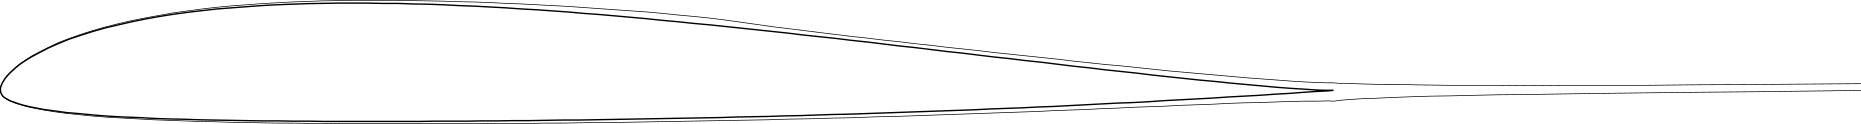
\includegraphics[width=.95\textwidth]{images/fileImg/alfa2_Re_25e4.png}} \\
\subfloat[][$\alpha=4^\circ$]
{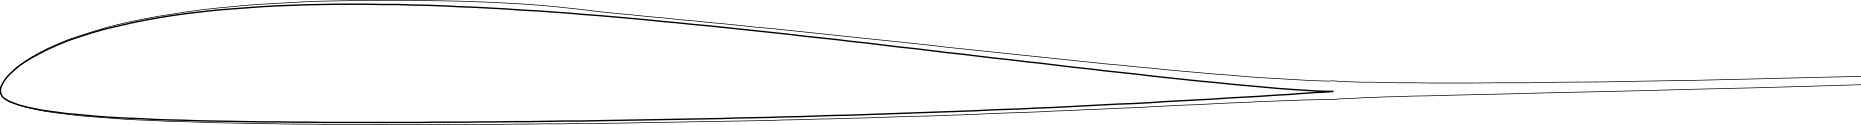
\includegraphics[width=.95\textwidth]{images/fileImg/alfa4_Re_25e4.png}} 
\caption{\footnotesize Profilo PW106, sviluppo dello strato limite, $Re=2.5\times10^5$, $n_{cr}$=9, transizione libera. XFOIL 6.99}
\label{fig:subfig}
\end{figure}


\noindent \\

Dalla figura~\vref{fig:subfig} si puó notare il lieve "rigonfiamento" dello strato limite in corrispondenza della bolla laminare che si sposta verso il bordo d'attacco all'aumentare di ${\alpha}$.\\ \\
Per studiare la dinamica delle bolle laminari, è necessario far riferimento all'evoluzione dei parametri di strato limite lungo il profilo. La presenza di una bolla, difatti, é accompagnata da una forte crescita del fattore di forma H come si vede in figura~\vref{fig:acca} e da un intervallo di valori negativo per quanto riguarda il coefficiente di attrito   $C_f$. La presenza delle bolle laminari è evidenziata da figura~\vref{fig:acca} a  figura~\vref{fig:fig4.13} mediante un'ellisse.

\begin{figure} [H]
\centering
\begin{tikzpicture} 
\begin{axis} [ 
legend style={at={(0.9,0.98)}},
ylabel style={rotate=-90}, xmin=0, 
xmax=2.02, 
ymin=0,
ymax=5,
xlabel=$\frac{s}{c}$, 
ylabel=$H$ ,
width=12cm,
height=7 cm,
scale only axis,
grid=major] 
\addplot [black,very thin,smooth]
file{images/fileDat/EffettiViscosi/H_alfa0_Re_25e4.dat};
\addplot [black,semithick, smooth]
file{images/fileDat/EffettiViscosi/H_alfa0_Re_5e5.dat};
\addplot [black,ultra thick,smooth]
file{images/fileDat/EffettiViscosi/H_alfa0_Re_1e6.dat};
\draw (0.4, 3) ellipse (0.2 and 1.9);
\legend {$Re=2.5\times10^5$,$Re=5\times10^5  $,$Re=1\times10^6$}
\end{axis}
\end{tikzpicture}
\caption{\footnotesize Profilo alare PW106, confronto dell'andamento del fattore di forma H al variare del numero di Reynolds, $\alpha=0^\circ$. XFOIL 6.99}\label{fig:acca}
\end{figure}
\noindent \\ \\ 



\begin{figure} [H]
\centering
\begin{tikzpicture} 
\begin{axis} [ 
ylabel style={rotate=-90}, xmin=0, 
xmax=2.02, 
ymin=-0.01,
ymax=0.04,
xlabel=$\frac{s}{c}$, 
ylabel=$C_f$ ,
width=12cm,
height=7 cm,
scale only axis,
grid=major] 
\addplot [black,very thin,smooth]
file{images/fileDat/EffettiViscosi/Cf_alfa0_Re_25e4.dat};
\addplot [black,semithick, smooth]
file{images/fileDat/EffettiViscosi/Cf_alfa0_Re_5e5.dat};
\addplot [black,ultra thick,smooth]
file{images/fileDat/EffettiViscosi/Cf_alfa0_Re_1e6.dat};
\draw (0.38, 0.002) ellipse (0.2 and 0.01);
\legend {$Re=2.5\times10^5$,$Re=5\times10^5  $,$Re=1\times10^6$}
\end{axis}
\end{tikzpicture}
\caption{\footnotesize Profilo alare PW106, confronto dell'andamento del coefficiente d'attrito $C_f$ al variare del numero di Reynolds, $\alpha=0^\circ$. XFOIL 6.99}\label{fig:cie}
\end{figure}
\noindent \\ \\ 

Dai grafici \ref{fig:acca} e \ref{fig:cie} si vede che a circa l' 60\% della corda, sul dorso del profilo, c'é una bolla laminare individuata da un intervallo di valori per i quali il $C_f$ è negativo per $Re=2.5 \times 10^5$ e $Re=5 \times 10^5$, ció non accade a numeri di Reynolds piú elevati.

È interessante, inoltre, vedere come variano i parametri di strato limite fissato il $Re$, a vari angoli d'attacco (figura~\vref{fig:fig4.12} e~\vref{fig:fig4.13}).

\begin{figure} [H]
\centering
\begin{tikzpicture} 
\begin{axis} [ 
ylabel style={rotate=-90}, xmin=0, 
xmax=2.02, 
ymin=0,
ymax=6.5,
xlabel=$\frac{s}{c}$,
ylabel=$H$ ,
width=12cm,
height=6.4 cm,
scale only axis,
grid=major] 
\addplot [black,very thin,smooth]
file{images/fileDat/EffettiViscosi/H_alfa0_Re_25e4.dat};
\addplot [black,semithick, smooth]
file{images/fileDat/EffettiViscosi/H_alfa2_Re_25e4.dat};
\addplot [black,ultra thick,smooth]
file{images/fileDat/EffettiViscosi/H_alfa4_Re_25e4.dat};
\draw (0.5, 3.1) ellipse (0.36 and 2.2);
\legend {$\alpha=0 $,$\alpha = 2$,$ \alpha=4$}
\end{axis}
\end{tikzpicture}
\caption{\footnotesize Profilo alare PW106, confronto dell'andamento del fattore di forma H al variare dell'angolo d'attacco, $Re=2.5\times10^5$. XFOIL 6.99 }
\label{fig:fig4.12}
\end{figure}
\noindent 

\begin{figure} [H]
\centering
\begin{tikzpicture} 
\begin{axis} [ 
ylabel style={rotate=-90}, xmin=0, 
xmax=2.02, 
ymin=-0.01,
ymax=0.07,
xlabel=$\frac{s}{c}$, 
ylabel=$C_f$ ,
width=12cm,
height=6.4 cm,
scale only axis,
grid=major] 
\addplot [black,very thin,smooth]
file{images/fileDat/EffettiViscosi/Cf_alfa0_Re_25e4.dat};
\addplot [black,semithick, smooth]
file{images/fileDat/EffettiViscosi/Cf_alfa2_Re_25e4.dat};
\addplot [black,ultra thick,smooth]
file{images/fileDat/EffettiViscosi/Cf_alfa4_Re_25e4.dat};
\draw (0.53, 0.002) ellipse (0.26 and 0.01);
\legend {$\alpha=0 $,$\alpha = 2$,$ \alpha=4$}
\end{axis}
\end{tikzpicture}
\caption{\footnotesize Profilo alare PW106, confronto dell'andamento del coefficiente d'attrito $C_f$ al variare dell'angolo d'attacco, $Re=2.5\times10^5$. XFOIL 6.99}
\label{fig:fig4.13}
\end{figure}
\noindent 

\section{Effetto della Transizione Forzata}
Forzare la transizione vuol dire anticipare il punto ove il flusso intorno al profilo diventa turbolento e, quindi, energizzarlo.\\
Se la transizione viene fissata prima della separazione, e, quindi, di un’eventuale bolla laminare, il flusso divenuto turbolento non separa più da laminare, determinando la scomparsa della bolla stessa.
Di seguito si esamineranno gli effetti della transizione forzata sul grafico del $C_p$ e sui grafici che descrivono i parametri di strato limite più significativi in tal senso: H e $C_f$.\\
Al fine di illustrare la scomparsa della bolla laminare a seguito di una transizione forzata che anticipa la separazione, si condurrà l’analisi a $Re=2.5\times10^5$ valore per il quale si è vista la presenza di una bolla laminare.

Sono stati assunti i seguenti valori:
\begin {itemize}
\item $Re=2.5\times10^5  $ ;
\item $ \alpha=2^\circ$.
\item $n_{cr}=9$
\end{itemize}
La transizione libera, calcolata con XFOIL, avviene (sul dorso) al seguente valore dell'ascissa adimensionalizzata con la corda: 
\begin{equation}
\frac{x_\mathrm{free-transit}}{c}= 0.539
\end {equation}
\noindent
È stata forzata la transizione sul dorso ad un valore di ${\frac{x}{c}}=0.300$ .\\
Di seguito sono riportati graficamente gli effetti che ne derivano.
\begin{figure} [H]
\centering
\begin{tikzpicture} 
\begin{axis} [ 
legend style={at={(0.98,0.98)}},
ylabel style={rotate=-90}, xmin=0, 
xmax=1, 
ymin=-1,
ymax=1,
xlabel=$\frac{x}{c}$, 
ylabel=$C_p$ ,
 y dir=reverse,
width=12cm,
height=7 cm,
scale only axis,
grid=major] 
\addplot [black,very thin]
file{images/fileDat/EffettiViscosi/Cp_alfa_2_Re_2.5_10e5dorso.dat};
\addplot [black, very thick]
file{images/fileDat/EffettiViscosi/Cp_alpha2_Re25e4_xtr0.3dorso.dat};
\addplot [black,very thin, dashed]
file{images/fileDat/EffettiViscosi/Cp_alfa_2_Re_2.5_10e5ventre.dat};
\addplot [black, very thick, dashed]
file{images/fileDat/EffettiViscosi/Cp_alpha2_Re25e4_xtr0.3ventre.dat};
\legend {$Transizione \ libera \ ( 53.9\%)$ , $Transizione \ forzata \ (30\%) $}
\end{axis}
\end{tikzpicture}
\caption{\footnotesize Profilo alare PW106, confronto del coefficiente di pressione sul dorso del profilo (linea continua) e sul ventre (linea tratteggiata) a diversi valori del punto di Transizione sul dorso.  $ \alpha=2^\circ$ , $ Re= 2.5\times10^5$. XFOIL 6.99}\label{fig:caso}
\end{figure}
\noindent

Dalle figure \ref{fig:nona} e \ref{fig:decima} si vede come anticipando la transizione il picco del fattore di forma dello strato limite H scompare e $C_f$ non assume valori negativi. Ciò conferma che non vi è più una bolla laminare sul dorso del profilo in quanto la transizione avviene prima della separazione.
\begin{figure} [H]
\centering
\begin{tikzpicture} 
\begin{axis} [ 
ylabel style={rotate=-90}, xmin=0, 
xmax=2.02, 
ymin=1,
ymax=6,
xlabel=$\frac{s}{c}$,
ylabel=$H$ ,
width=12cm,
height=7cm,
scale only axis,
grid=major] 
\addplot [black,very thin,smooth]
file{images/fileDat/EffettiViscosi/H_alfa2_Re_25e4.dat};
\addplot [black,very thick, smooth]
file{images/fileDat/EffettiViscosi/H_alfa2_Re_25e4_xtr0.3.dat};
\legend {$Transizione \ libera \ ( 53.9\%)$ , $Transizione \ forzata \ (30\%) $}
\end{axis}
\end{tikzpicture}
\caption{\footnotesize Profilo PW106, confronto dell'andamento del fattore di forma H al variare del punto di Transizione sul dorso.  $ \alpha=2^\circ$ , $ Re= 2.5\times10^5$. XFOIL 6.99}\label{fig:decima}
\end{figure} 

\begin{figure} [H]
\centering
\begin{tikzpicture} 
\begin{axis} [ 
legend style={at={(0.98,0.98)}},
ylabel style={rotate=-90}, xmin=0, 
xmax=2.02, 
ymin=-0.01,
ymax=0.05,
xlabel=$\frac{s}{c}$,
ylabel=$C_f$ ,
width=12cm,
height=7.5cm,
scale only axis,
grid=major] 
\addplot [black,very thin,smooth]
file{images/fileDat/EffettiViscosi/Cf_alfa2_Re_25e4.dat};
\addplot [black,very thick, smooth]
file{images/fileDat/EffettiViscosi/Cf_alfa2_Re_25e4_xtr0.3.dat};
\legend {$Transizione \ libera \ ( 53.9\%)$ , $Transizione \ forzata \ (30\%) $}
\end{axis}
\end{tikzpicture}
\caption{\footnotesize Profilo PW106, confronto dell'andamento del Coefficiente d'attrito $C_f$ al variare del punto di Transizione sul dorso.  $ \alpha=2^\circ$ , $ Re= 2.5\times10^5$. XFOIL 6.99}\label{fig:nona}
\end{figure}
\noindent 

\section{Effetto della variazione di $n_{cr}$}

Gli effetti della turbolenza asintotica, della rugosità del profilo e di altri disturbi sono tenuti in considerazione tramite un parametro $n_{cr}$, detto {\itshape fattore di amplificazione}.\\ Di {\itshape default} $n_{cr}$ su XFOIL è fissato a 9. In questo paragrafo analizzeremo gli effetti di una variazione di $n_{cr}$, per valori maggiori e minori di 9.\\
Per $n_{cr} > 9$ , la transizione dello strato limite da laminare a turbolento posticiperà , mentre anticiperà per $n_{cr} < 9$ con tutto ciò che ne consegue sulla stabilità dello strato limite e la presenza di bolle laminari già esposto nel paragrafo precedente.\\ \\
Assunti i seguenti valori:

\begin {itemize}
\item $Re=2.5\times10^5  $ 
\item $ \alpha=2^\circ$
\end{itemize}
\noindent 
Si pone  $n_{cr}=3, 9, 15$ per calcolare il $C_p$, H e $C_f$ .

\noindent \\

\begin{figure} [H]
\centering
\begin{tikzpicture} 
\begin{axis} [ 
legend style={at={(0.33,0.4)}},
ylabel style={rotate=-90}, xmin=0, 
xmax=1, 
ymin=-1,
ymax=1,
xlabel=$\frac{x}{c}$, 
ylabel=$C_p$ ,
 y dir=reverse,
width=13cm,
height=8.5cm,
scale only axis,
grid=major] 
\addplot [black,very thin]
file{images/fileDat/EffettiViscosi/Cp_alfa_2_Re_2.5_10e5_n3dorso.dat};
\addplot [black, semithick]
file{images/fileDat/EffettiViscosi/Cp_alfa_2_Re_2.5_10e5dorso.dat};
\addplot [black, ultra thick]
file{images/fileDat/EffettiViscosi/Cp_alfa_2_Re_2.5_10e5_n15dorso.dat};
\addplot [black,very thin, dashed]
file{images/fileDat/EffettiViscosi/Cp_alfa_2_Re_2.5_10e5_n3ventre.dat};
\addplot [black, semithick, dashed]
file{images/fileDat/EffettiViscosi/Cp_alfa_2_Re_2.5_10e5ventre.dat};
\addplot [black, ultra thick, dashed]
file{images/fileDat/EffettiViscosi/Cp_alfa_2_Re_2.5_10e5_n15ventre.dat};
\legend {$n_{cr}=3$,$n_{cr}=9$,$n_{cr}=15$}
\end{axis}
\end{tikzpicture}
\caption{\footnotesize Profilo PW106, confronto del coefficiente di pressione sul dorso del profilo (linea continua) e sul ventre (linea tratteggiata) a diversi valori del fattore di amplificazione.  $ \alpha=2^\circ$ , $ Re= 2.5\times10^5$. XFOIL 6.99}\label{fig:n}
\end{figure}

\begin{figure} [H]
\centering
\begin{tikzpicture} 
\begin{axis} [ 
ylabel style={rotate=-90}, xmin=0, 
xmax=2.02, 
ymin=0,
ymax=10,
xlabel=$\frac{s}{c}$, 
ylabel=$H$ ,
width=12cm,
height=7.5cm,
scale only axis,
grid=major] 
\addplot [black,ultra thin]
file{images/fileDat/EffettiViscosi/H_alfa2_Re_25e4_n3.dat};
\addplot [black, semithick]
file{images/fileDat/EffettiViscosi/H_alfa2_Re_25e4.dat};
\addplot [black, ultra thick]
file{images/fileDat/EffettiViscosi/H_alfa2_Re_25e4_n15.dat};
\legend {$n=3$,$n=9 $,$n=15$}
\end{axis}
\end{tikzpicture}
\caption{\footnotesize Profilo PW106, confronto dell'andamento del fattore di forma H al variare del fattore di amplificazione.  $ \alpha=2^\circ$ , $ Re= 2.5\times10^5$. XFOIL 6.99}\label{fig:n1}
\end{figure}

\begin{figure} [H]
\centering
\begin{tikzpicture} 
\begin{axis} [ 
legend style={at={(0.996,0.98)}},
ylabel style={rotate=-90}, xmin=0, 
xmax=2.02, 
ymin=-0.01,
ymax=0.04,
xlabel=$\frac{s}{c}$,
ylabel=$C_f$ ,
width=12cm,
height=7.5cm,
scale only axis,
grid=major] 
\addplot [black,ultra thin]
file{images/fileDat/EffettiViscosi/Cf_alfa2_Re_25e4_n3.dat};
\addplot [black, semithick]
file{images/fileDat/EffettiViscosi/Cf_alfa2_Re_25e4.dat};
\addplot [black, ultra thick]
file{images/fileDat/EffettiViscosi/Cf_alfa2_Re_25e4_n15.dat};
\legend {$n=3$,$n=9 $,$n=15$}
\end{axis}
\end{tikzpicture}
\caption{\footnotesize Profilo PW106, confronto dell'andamento del Coefficiente d'attrito $C_f$ al variare del fattore di amplificazione.  $ \alpha=2^\circ$ , $ Re= 2.5\times10^5$. XFOIL 6.99}\label{fig:n1}
\end{figure}
%   % !TeX program = PdfLaTeX
% !TeX root = ../../Elaborati_Aerodinamica_Bruno_Spoti.tex
\chapter{Aerodinamica viscosa alle alte incidenze}
In questo capitolo saranno svolti calcoli viscosi in condizioni di alta portanza considerando un $Re=1\times10^6$.
Dalla curva di portanza in figura~\vref{fig:cla11} si vede che per questo valore di $Re$ $ {\alpha}_{stall}=13^\circ$. In questa sede si utilizzerà un  {\bfseries $\alpha=12^\circ$} per meglio visualizzare i fenomeni legati alla viscositá.\\ 
In primo luogo sarà graficata la distribuzione del $C_p$ all’angolo di alta portanza scelto. Successivamente saranno analizzati i parametri di strato limite, in termini di H, ${\delta^*}$, ${\theta}$ e $C_f$ in condizioni di piccoli angoli d’attacco e in condizioni di alta portanza. Saranno poi analizzati gli effetti della turbolenza asintotica e della transizione forzata. Infine sarà valutato lo stallo del profilo secondo il criterio semiempirico di Thain e Gault al variare del numero di Reynolds.
\section{Coefficiente di pressione}
\begin{figure} [H]
\centering
\begin{tikzpicture} 
\begin{axis} [ 
ylabel style={rotate=-90}, xmin=0, 
xmax=1, 
ymin=-10,
ymax=2,
xlabel=$\frac{x}{c}$, 
ylabel=$C_p$ ,
 y dir=reverse,
width=12cm,
height=5 cm,
scale only axis,
grid=major] 
\addplot [black,thick, smooth]
file{images/fileDat/EffettiViscosiAlteIncidenze/Cp_alfa_12_Re_1_10e6dorso.dat};
\addplot [black,thick, smooth, dashed]
file{images/fileDat/EffettiViscosiAlteIncidenze/Cp_alfa_12_Re_1_10e6ventre.dat};
\addplot [black,thin,smooth]
file{images/fileDat/EffettiViscosiAlteIncidenze/Cp_alfa_4_Re_1_10e6dorso.dat};
\addplot [black,thin, smooth, dashed]
file{images/fileDat/EffettiViscosiAlteIncidenze/Cp_alfa_4_Re_1_10e6ventre.dat};
\legend {$ \alpha=12^\circ$,$ \alpha=4^\circ$}
\end{axis}
\end{tikzpicture}
\caption{\footnotesize Profilo alare PW106, confronto del coefficiente di pressione $ \alpha=12^\circ$,$ \alpha=4^\circ$. $Re=1\times10^6$. XFOIL 6.99}
\end{figure}

\section{Sviluppo e Parametri di strato limite}
Tramite XFOIL è stato valutato come si sviluppa lo strato limite ad aumentare dell’angolo d’attacco dalle basse incidenze fino ad oltre lo stallo.\\ 
Si nota che all'aumentare del numero di Reynolds la zona di flusso separato sul dorso del profilo si espande sempre più  verso il bordo d'attacco.
\begin{figure}[H]
\centering
\subfloat[][$\alpha=4^\circ$]
{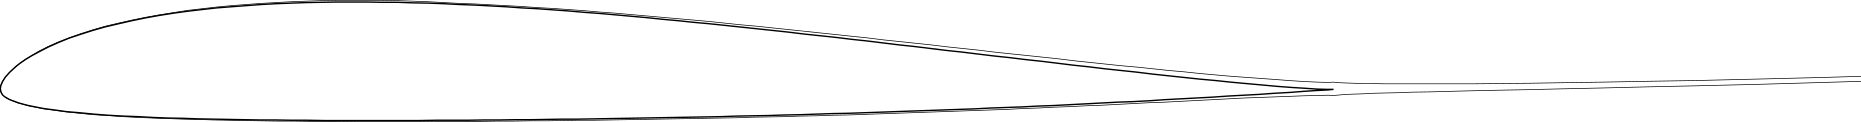
\includegraphics[width=.95\textwidth]{images/fileImg/alfa4_Re_1e6.png}} \\
\subfloat[][$\alpha=12^\circ$]
{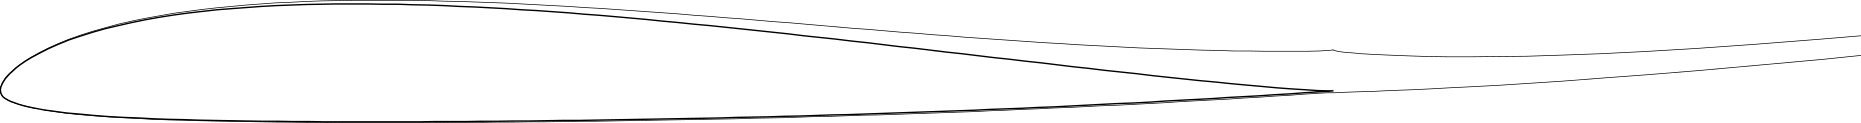
\includegraphics[width=.95\textwidth]{images/fileImg/alfa12_Re_1e6.png}} \\
\subfloat[][$\alpha=19^\circ$]
{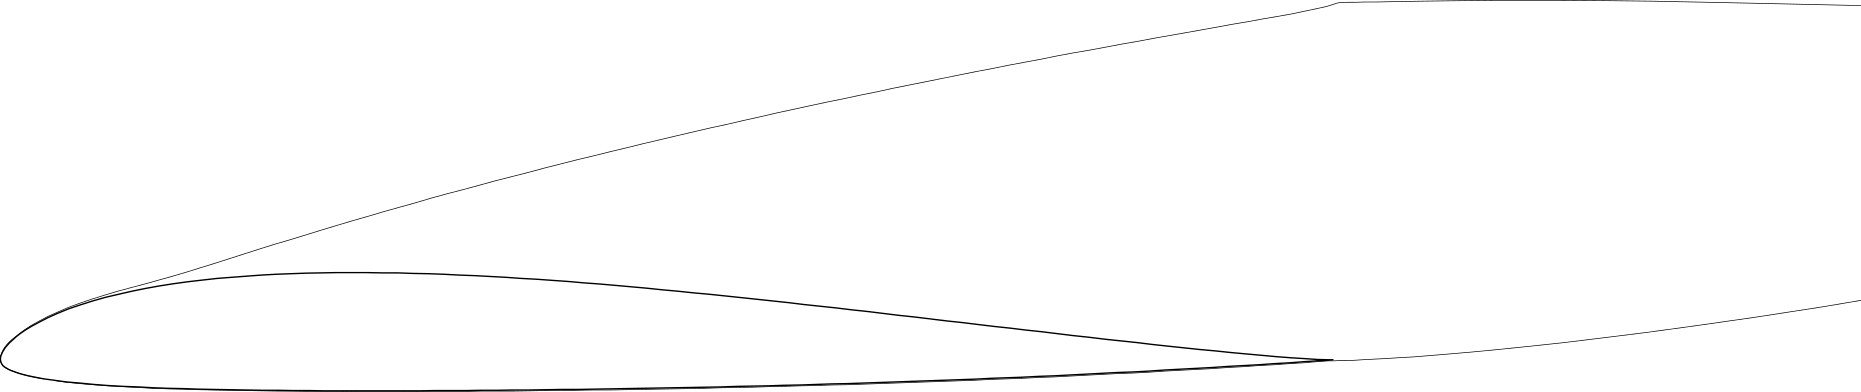
\includegraphics[width=.95\textwidth]{images/fileImg/alfa19_Re_1e6.png}} 
\caption{\footnotesize Profilo PW106, sviluppo dello strato limite, $Re=1\times10^6$, $n_{cr}$=9, transizione libera. XFOIL 6.99}
\label{fig:subfig2}
\end{figure}

Lo strato limite è univocamente definito assegnata la terna H, ${\delta^*}$, ${\theta}$. Di seguito sará studiata la variazione di questi parametri con l’angolo d’attacco congiuntamente allo studio della variazione del coefficiente d’attrito.\\
Si noti che sul ventre del profilo a nessuna incidenza si verificano particolari fenomeni di separazione e il flusso resta laminare.

\begin{figure} [H]
\centering
\begin{tikzpicture} 
\begin{axis} [ 
ylabel style={rotate=-90}, xmin=0, 
xmax=2.02, 
ymin=0,
ymax=10,
xlabel=$\frac{s}{c}$,
ylabel=$H$ ,
width=12cm,
height=8.5 cm,
scale only axis,
grid=major] 
\addplot [black,very thin,smooth]
file{images/fileDat/EffettiViscosiAlteIncidenze/H_alfa4_Re_1e6.dat};
\addplot [black,very thick, smooth]
file{images/fileDat/EffettiViscosiAlteIncidenze/H_alfa12_Re_1e6.dat};
\legend { $ \alpha=4^\circ$,$ \alpha=12^\circ$}
\end{axis}
\end{tikzpicture}
\caption{\footnotesize Profilo alare PW106, confronto dell'andamento del fattore di forma H al variare dell'angolo d'attacco. XFOIL 6.99}
\end{figure}
\noindent


\begin{figure} [H]
\centering
\begin{tikzpicture} 
\begin{axis} [ 
ylabel style={rotate=-90}, xmin=0, 
xmax=2.02, 
ymin=-0.01,
ymax=0.1,
xlabel=$\frac{s}{c}$,
ylabel=$C_f$ ,
width=12cm,
height=8.5 cm,
scale only axis,
grid=major] 
\addplot [black,very thin,smooth]
file{images/fileDat/EffettiViscosiAlteIncidenze/Cf_alfa4_Re_1e6.dat};
\addplot [black,very thick, smooth]
file{images/fileDat/EffettiViscosiAlteIncidenze/Cf_alfa12_Re_1e6.dat};;
\legend { $ \alpha=4^\circ$,$ \alpha=12^\circ$}
\end{axis}
\end{tikzpicture}
\caption{\footnotesize Profilo alare PW106, confronto dell'andamento del Coefficiente d'attrito $C_f$ al variare dell'angolo d'attacco. XFOIL 6.99}
\end{figure}
\noindent \\ \\ 

Il particolare andamento del coefficiente d'attrito e del fattore di forma per $ \alpha=12^\circ$ è deducibile da un’analisi dello sviluppo dello strato limite alle alte incidenze. Nel punto di ristagno anteriore la velocità locale è nulla, quindi sarà nullo anche il numero di Reynolds locale, calcolato rispetto la distanza dal {\itshape nose}. Ciò vuol dire che ivi le $\tau$ sono molto alte e, pertanto, sono in grado di annichilire ogni disturbo. In questo punto si avrà, quindi, un $C_f$ molto alto e un H piuttosto basso. Procedendo verso il TE sul dorso si incontra una bolla laminare alla quale corrisponde un intervallo di $C_f$ negativi e un picco nel fattore di forma. La bolla comporta una separazione laminare, ma anche la transizione a turbolento che energizza il flusso e consente il riattacco con un conseguente aumento di $C_f$. Si ha così un flusso turbolento attaccato più energizzato, che porta ad una diminuzione di H. L'alta incidenza non consente di avere un flusso attaccato per un ampio intervallo di profilo e quindi separa, facendo si che H cresca fino al TE.

\begin{figure} [H]
\centering
\begin{tikzpicture} 
\begin{axis} [ 
ylabel style={rotate=-90}, xmin=0, 
xmax=2.02, 
ymin=-0.01,
ymax=0.015,
xlabel=$\frac{s}{c}$,
ylabel= ${\theta}$ ,
width=0.9\textwidth,
height=6cm,
scale only axis,
grid=major] 
\addplot [black,very thin,smooth]
file{images/fileDat/EffettiViscosiAlteIncidenze/Theta_alfa4_Re_1e6.dat};
\addplot [black,very thick, smooth]
file{images/fileDat/EffettiViscosiAlteIncidenze/Theta_alfa12_Re_1e6.dat};;
\legend { $ \alpha=4^\circ$,$ \alpha=12^\circ$}
\end{axis}
\end{tikzpicture}
\caption{\footnotesize Profilo alare PW106, confronto dell'andamento dello spessore di quantità di moto  ${\theta}$ al variare dell'angolo d'attacco. XFOIL 6.99}
\end{figure}
\begin{figure} [H]
\centering
\begin{tikzpicture} 
\begin{axis} [ 
ylabel style={rotate=-90}, xmin=0, 
xmax=2.02, 
ymin=-0.01,
ymax=0.05,
xlabel=$\frac{s}{c}$, 
ylabel=${\delta^*}$ ,
width=0.9\textwidth,
height=6cm,
scale only axis,
grid=major] 
\addplot [black,very thin,smooth]
file{images/fileDat/EffettiViscosiAlteIncidenze/Delta_star_alfa4_Re_1e6.dat};
\addplot [black,very thick, smooth]
file{images/fileDat/EffettiViscosiAlteIncidenze/Delta_star_alfa12_Re_1e6.dat};;
\legend { $ \alpha=4^\circ$,$ \alpha=12^\circ$}
\end{axis}
\end{tikzpicture}
\caption{\footnotesize Profilo alare PW106, confronto dell'andamento dello spessore di spostamento ${\delta^*}$ al variare dell'angolo d'attacco. XFOIL 6.99}
\end{figure}
\noindent \\ \\ 



\section{Effetto della variazione del numero di Reynolds e stallo}

Da uno zoom sul grafico della curva di portanza, si può notare come il $C_{l_\mathrm{max}}$ cresce all'aumentare del numero di Reynolds con un conseguente aumento dell'${\alpha}_{stall}$
Nella tabella \ref{tab:rei} sono riportati i valori dell'angolo di stallo e del $C_{l_\mathrm{max}}$ a vari numeri di Reynolds.

\begin{table}[htbp]\centering \rowcolors{1}{}{grigio_chiaro}
\begin{tabular}{c S c c}
\toprule
\emph{Numero di Reynolds} & $ C_{l_\mathrm{max}}$  & ${\alpha}_\mathrm{stall}$  \\
\midrule
$5\times10^5$ & 1.28 & $13^\circ$ \\
$1\times10^6$ & 1.38 & $13^\circ$ \\
$3\times10^6 $ & 1.56 & $16^\circ$ \\
$1\times10^7 $& 1.76 & $18^\circ$ \\
\bottomrule
\end{tabular}
\caption {$C_{l_\mathrm{max}}$ e ${\alpha}_\mathrm{stall}$ al variare del numero di Reynolds}
\label{tab:rei}
\end{table}
\begin{figure} [H]
\centering
\begin{tikzpicture} 
\begin{axis} [ 
legend style={at={(0.45,0.98)}},
ylabel style={rotate=-90}, xmin=8, 
xmax=25, 
ymin=1,
ymax=2,
xlabel=${\alpha}$,
ylabel=$C_l$ ,
width=8cm,
height=9.5 cm,
scale only axis,
grid=major] 
\addplot [black, smooth,mark=*]
file{images/fileDat/EffettiViscosi/Cl_vs_alpha_Re_5_10_5.dat};
\addplot [black,smooth,mark=square]
file{images/fileDat/EffettiViscosi/Cl_vs_alpha_Re_1_10_6.dat};
\addplot [black, smooth,mark=diamond*]
file{images/fileDat/EffettiViscosi/Cl_vs_alpha_Re_3_10_6.dat};
\addplot [black, smooth,mark=star]
file{images/fileDat/EffettiViscosi/Cl_vs_alpha_Re_1_10_7.dat};
\legend {$Re=5\times10^5  $,$Re=1\times10^6$,$Re=3\times10^6$,$Re=1\times10^7$}
\end{axis}
\end{tikzpicture} 
\caption{\footnotesize Confronto delle curve di Portanza del profilo PW106 a vari numeri di Reynolds, zoom della zona di stallo. XFOIL 6.99}
\label{fig:cla2}
\end{figure}



Di seguito sarà analizzato l'andamento del $C_p$ allo stallo per diversi numeri di Reynolds al fine di vedere che tipo di stallo interessa il profilo in date condizioni.

\begin{figure} [H]
\centering
\begin{tikzpicture} 
\begin{axis} [ 
ylabel style={rotate=-90}, xmin=0, 
xmax=1, 
ymin=-17,
ymax=1.2,
xlabel=$\frac{x}{c}$, 
ylabel=$C_p$ ,
 y dir=reverse,
width=13cm,
height=7cm,
scale only axis,
grid=major] 
\addplot [black,very thick]
file{images/fileDat/EffettiViscosiAlteIncidenze/Cp_stall_Re5e5dorso.dat};
\addplot [black, semithick]
file{images/fileDat/EffettiViscosiAlteIncidenze/Cp_stall_Re1e6dorso.dat};
\addplot [black, thin]
file{images/fileDat/EffettiViscosiAlteIncidenze/Cp_stall_Re1e7dorso.dat};
\addplot [black,very thick, dashed]
file{images/fileDat/EffettiViscosiAlteIncidenze/Cp_stall_Re5e5ventre.dat};
\addplot [black, semithick, dashed]
file{images/fileDat/EffettiViscosiAlteIncidenze/Cp_stall_Re1e6ventre.dat};
\addplot [black, thin, dashed]
file{images/fileDat/EffettiViscosiAlteIncidenze/Cp_stall_Re1e7ventre.dat};
\legend {$Re=5\times10^5$,$Re=1\times10^6$,$Re=10\times10^6$}
\end{axis}
\end{tikzpicture}
\caption{\footnotesize Profilo alare PW106, confronto del coefficiente di pressione allo stallo sul dorso del profilo (linea continua) e sul ventre (linea tratteggiata) a diversi valori numero di Reynolds. XFOIL 6.99 }\label{fig:stall}
\end{figure}
\noindent \\


\begin{figure} [H]
\centering
\begin{tikzpicture} 
\begin{axis} [ 
ylabel style={rotate=-90}, xmin=0, 
xmax=0.05, 
ymin=-10,
ymax=-6,
xlabel=$\frac{x}{c}$, 
ylabel=$C_p$ ,
 y dir=reverse,
width=10cm,
height=6cm,
scale only axis,
grid=major] 
\addplot [black,very thick]
file{images/fileDat/EffettiViscosiAlteIncidenze/Cp_stall_Re5e5dorso.dat};
\addplot [black, semithick]
file{images/fileDat/EffettiViscosiAlteIncidenze/Cp_stall_Re1e6dorso.dat};
\addplot [black, thin]
file{images/fileDat/EffettiViscosiAlteIncidenze/Cp_stall_Re1e7dorso.dat};
\addplot [black,very thick, dashed]
file{images/fileDat/EffettiViscosiAlteIncidenze/Cp_stall_Re5e5ventre.dat};
\addplot [black, semithick, dashed]
file{images/fileDat/EffettiViscosiAlteIncidenze/Cp_stall_Re1e6ventre.dat};
\addplot [black, thin, dashed]
file{images/fileDat/EffettiViscosiAlteIncidenze/Cp_stall_Re1e7ventre.dat};
\legend {$Re=5\times10^5$,$Re=1\times10^6$,$Re=10\times10^6$}
\end{axis}
\end{tikzpicture}
\caption{\footnotesize Profilo alare PW106, zoom del particolare nel confronto del coefficiente di pressione allo stallo a diversi valori numero di Reynolds. XFOIL 6.99}\label{fig:stallz}
\end{figure}
\noindent \\


%Dalle figure  \ref{fig:stall} e  \ref{fig:stallz} si può notare il diverso comportamento del profilo in condizioni di stallo al variare del numero di Reynolds. \\Per $Re=5\times10^5$ si può osservare la formazione di una bolla laminare sul dorso del profilo, verso il LE. %Tale bolla ha un’estensione di circa il $20\%$ della corda.
%Ciò può essere confermato dall’intervallo di valori negativi del coefficiente di attrito diagrammati in figura \ref{fig:coef} cui corrisponde un picco nel diagramma di H come si vede in figura \ref{fig:h}.
%Per $Re=1\times10^6$ si ha una bolla più corta che potrebbe esser causa di uno stallo da esplosione da bolla, più violento. Aumentando il numero di Reynolds, fino ad un valore di $Re=10\times10^6$ la bolla scompare cosicché il profilo è caratterizzato da uno stallo turbolento.\\
%È possibile verificare queste considerazioni nei grafici  riportati in figura~\vref{fig:h} e~\vref{fig:coef} che esprimono i parametri di strato limite più significativi in tal senso. Alla presenza di una bolla corrispondono zone di $C_f$  negative piú o meno estese e picchi nel fattore di forma H.
%
%\noindent \\  \\



\begin{figure} [H]
\centering
\begin{tikzpicture} 
\begin{axis} [ 
ylabel style={rotate=-90}, xmin=0, 
xmax=2.02, 
ymin=0,
ymax=13,
xlabel=$\frac{s}{c}$,
ylabel=$H$ ,
width=12cm,
height=9 cm,
scale only axis,
grid=major] 
\addplot [black,very thick]
file{images/fileDat/EffettiViscosiAlteIncidenze/H_stall_Re5e5.dat};
\addplot [black, semithick]
file{images/fileDat/EffettiViscosiAlteIncidenze/H_stall_Re1e6.dat};
\addplot [black, very thin]
file{images/fileDat/EffettiViscosiAlteIncidenze/H_stall_Re1e7.dat};
\legend {$Re=5\times10^5$,$Re=1\times10^6$,$Re=10\times10^6$}
\end{axis}
\end{tikzpicture}
\caption{\footnotesize Profilo alare PW106, confronto dell'andamento del fattore di forma H allo stallo al variare del numero di Reynolds. XFOIL 6.99}
\label{fig:h}
\end{figure}
\noindent


\begin{figure} [H]
\centering
\begin{tikzpicture} 
\begin{axis} [ 
ylabel style={rotate=-90}, xmin=0, 
xmax=2.02, 
ymin=-0.01,
ymax=0.14,
xlabel=$\frac{s}{c}$,
ylabel=$C_f$ ,
width=12cm,
height=7cm,
scale only axis,
grid=major] 
\addplot [black,very thick]
file{images/fileDat/EffettiViscosiAlteIncidenze/Cf_stall_Re5e5.dat};
\addplot [black, semithick]
file{images/fileDat/EffettiViscosiAlteIncidenze/Cf_stall_Re1e6.dat};
\addplot [black, very thin]
file{images/fileDat/EffettiViscosiAlteIncidenze/Cf_stall_Re1e7.dat};
\legend {$Re=5\times10^5$,$Re=1\times10^6$,$Re=10\times10^6$}
\end{axis}
\end{tikzpicture}
\caption{\footnotesize Profilo alare PW106, confronto dell'andamento del coefficiente d'attrito $C_f$ allo stallo al variare del numero di Reynolds. XFOIL 6.99}
\label{fig:coef}
\end{figure}
 \noindent \\ 


Applicando il criterio semiempirico di stallo di Thain e Gault e possibile fare una previsione del tipo di stallo.\\
In particolare per verificare il tipo di stallo è stato calcolato lo spessore percentuale del profilo ad ${\frac {x}{c} }=0.0125$ ottenendo un valore di $1.75 \%$ entrando, in tal modo, nel grafico riportato in figura~\vref{fig:tin}.



\begin {figure} [H]
\centering
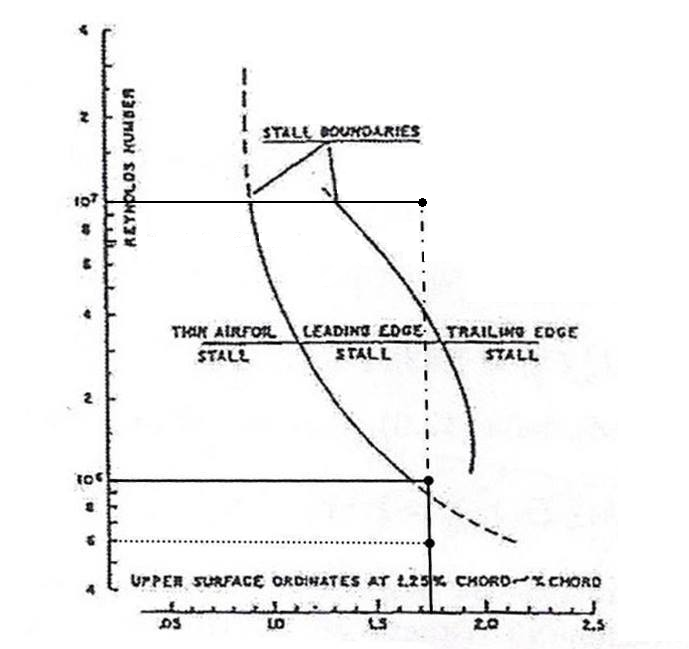
\includegraphics[width= 12cm ]{images/fileImg/thin.png}
\caption{\footnotesize Criterio di Thain e Gault, risultati per il profilo PW106}
\label {fig:tin}
\end {figure}

\begin{figure} [H]
	\centering
	\begin{tikzpicture} 
	\begin{semilogyaxis} [ 
	ylabel style={rotate=-90}, xmin=0.3, 
	xmax=2.5, 
	ymin=300000,
	ymax=40000000,
	xlabel=$\frac{s}{c}$,
	ylabel=$C_f$ ,
	width=10cm,
	height=12cm,
	scale only axis] 
	\addplot [black,very thick,smooth]
	file{images/fileDat/EffettiViscosiAlteIncidenze/StallBoundary1.dat};
	\addplot [black,very thick,smooth]
	file{images/fileDat/EffettiViscosiAlteIncidenze/StallBoundary2.dat};
		\node at (axis cs: 0.4, 0.07) { \scriptsize Regione 1};
	\node at (axis cs: 0.7, 3000000) { \scriptsize THIN AIRFOIL};
	\node at (axis cs: 1.45, 3000000) { \scriptsize LEADING EDGE};
	\node at (axis cs: 2.1, 3000000) { \scriptsize TRAILING EDGE};
		\node at (axis cs: 0.7, 2500000) { \scriptsize STALL};
	\node at (axis cs: 1.45, 2500000) { \scriptsize STALL};
	\node at (axis cs: 2.1, 2500000) { \scriptsize STALL};
	\node at (axis cs: 0.8, -0.1) { \scriptsize Regione 5};
	\node at (axis cs: 1.3, 0.04) { \scriptsize Regione 3};
	\node at (axis cs: 1.3, -0.05) { \scriptsize Regione 6};
	\end{semilogyaxis}
	\end{tikzpicture}
	\caption{\footnotesize Profilo alare PW106, confronto dell'andamento del coefficiente d'attrito $C_f$ allo stallo al variare del numero di Reynolds. XFOIL 6.99}
	\label{fig:coef}
\end{figure}
\noindent \\ 

%   % !TeX program = PdfLaTeX
% !TeX root = ../../Elaborati_Aerodinamica_Bruno_Spoti.tex
\chapter{Modifiche della geometria}

In questo capitolo verranno apportate delle modifiche alla geometria del profilo tramite XFOIL al fine di studiarne la configurazione con {\itshape flap} e Alettoni.\\ Tramite la funzione {\itshape f}, nel menu {\itshape GDES} di XFOIL è possibile deflettere parte del profilo così da simulare un {\itshape plain flap}.
Di seguito saranno riportate le curve di portanza, le polari, la distribuzione del coefficiente di pressione e i principali risultati numerici per diverse deflessioni dignificative delle superfici mobili.

\section {Configurazione con {\itshape Flap}}

Per studiare il comportamento del profilo con {\itshape flap} è stata prevista una deflessione di  $25^\circ $, compatibilmente con dati verosimili in condizione di atterraggio. La corda del flap è stata scelta pari al 30\% della corda del profilo.\\
Lo scopo del flap è quello di aumentare il $C_{l_{\mathrm{max}}}$ del profilo, ottenendo, però, anche uno stallo ad angoli d'attacco più bassi. Con flap parzialmente aperti (dai $10^\circ $ ai $20^\circ $) l’effetto risultante è un forte aumento di portanza e un relativamente piccolo incremento di resistenza. Per flap con deflessioni più ampie si ha anche un forte aumento di resistenza. In tabella~\ref{tab:flap} sono riportati gli effetti della deflessione dei flap, in termini di $C_{l_{max}}$ e angolo di stallo per $Re=1\times10^6$, in caso incomprimibile.\\

\begin{table} [!h]\centering \rowcolors{1}{}{grigio_chiaro}
\begin{tabular}{c S c c}
\toprule
\emph{Angolo di deflessione dei flap} &  $C_{l_{\mathrm{max}}}$  &  ${\alpha}_{\mathrm{stall}}$ & ${\alpha}_{\mathrm{zl}}$  \\ 
\midrule
$\delta_{\mathrm{flap}}=0^\circ$ & 1.37 & $13.1^\circ$  & $-0.873^\circ$  \\
$\delta_{\mathrm{flap}}=25^\circ$ & 1.75 & $7.41^\circ$ & $-14.7^\circ$  \\
\bottomrule
\end{tabular}
\caption {Profilo alare PW106, $C_{l_{\mathrm{max}}}$, ${\alpha}_{\mathrm{stall}}$ e ${\alpha}_{\mathrm{zl}}$ per flap retratto e deflesso, $ Re=1\times10^6$.}
\label{tab:flap}
\end{table}


\begin{figure}
\centering
\begin{tikzpicture} 
\begin{axis} [ 
ylabel style={rotate=-90}, xmin=0, 
xmax=1, 
ymin=-0.2,
 ymax=0.1,
 xlabel=$ \frac {x}{c}$, 
ylabel=$ \frac {z}{c}$,
ytick={-0.2,-0.1,0,0.1},
yticklabels={$-0.2$,$-0.1$,$0$,$0.1$},
width=13cm,
 height=3.9 cm,
scale only axis,
grid=major] 
\addplot [black,solid,very thin]
file{images/fileDat/FlapsAlettoni/ProfiloPW106Chiuso.dat};
\addplot [black,solid,very thick]
file{images/fileDat/FlapsAlettoni/PW106FlapTakeOff.dat};
\end{axis}
\end{tikzpicture}
\caption{\footnotesize Profilo alare PW106, configurazione con flap per $\delta_{flap}=25 ^\circ$  }
\end{figure}


\begin{figure} [H]
\centering
\begin{tikzpicture} 
\begin{axis} [ 
legend style={at={(0.35,0.98)}},
ylabel style={rotate=-90}, xmin=-18, 
xmax=18, 
ymin=0,
ymax=2,
xlabel=${\alpha}$,
ylabel=$C_l$ ,
width=10cm,
height=12.5 cm,
scale only axis,
grid=major] 
\addplot [black, smooth, thick]
file{images/fileDat/FlapsAlettoni/clFlapClean.dat};
\addplot [black,smooth,mark=*, thick]
file{images/fileDat/FlapsAlettoni/ClFlap25.dat};
\legend {$\delta_{flap}=0 ^\circ$,$\delta_{flap}=25 ^\circ$}
\end{axis}
\end{tikzpicture} 
\caption{\footnotesize Profilo alare PW106,  confronto delle curve di portanza del profilo per $ Re=1\times10^6$ per flap deflessi e in configurazione pulita. XFOIL 6.99 }
\label{fig:flappi}
\end{figure}

\begin{figure} [H]
\centering
\begin{tikzpicture} 
\begin{axis} [ 
ylabel style={rotate=-90}, xmin=0, 
xmax=1, 
ymin=-7,
ymax=1,
xlabel=$\frac{x}{c}$, 
ylabel=$C_p$ ,
 y dir=reverse,
width=12cm,
height=8 cm,
scale only axis,
grid=major] 
\addplot [black,thin]
file{images/fileDat/FlapsAlettoni/Cp_alfa_4_Re_1_10e6dorso.dat};
\addplot [black,ultra thick]
file{images/fileDat/FlapsAlettoni/PW106CP4degdorso.dat};
\addplot [black,thin,dashed]
file{images/fileDat/FlapsAlettoni/Cp_alfa_4_Re_1_10e6ventre.dat};
\addplot [black,ultra thick,dashed]
file{images/fileDat/FlapsAlettoni/PW106CP4degventre.dat};
\legend {$\delta_{flap}=0 ^\circ$,  $\delta_{flap}=25 ^\circ$}
\end{axis}
\end{tikzpicture}
\caption{\footnotesize Profilo alare PW106, confronto del Coefficiente di Pressione con flap deflessi $\delta_{flap}=25 ^\circ$ e configurazione pulita. $Re=1\times10^6$ $\alpha =4 ^\circ$ }
\end{figure}

\begin{figure} [H]
\centering
\begin{tikzpicture} 
\begin{axis} [ 
legend style={at={(0.98,0.20)}},
ylabel style={rotate=-90}, xmin=0, 
ymin=-1,
ymax=2,
xlabel=$C_d$,
ylabel=$C_l$ ,
width=11cm,
height=8cm,
scale only axis,
grid=major] 
\addplot [black, smooth,thick]
file{images/fileDat/FlapsAlettoni/cd_cl_10_6.dat};
\addplot [black,smooth,mark=square]
file{images/fileDat/FlapsAlettoni/CdFlapTo.dat};
\legend {$\delta_{flap}=0 ^\circ$,$\delta_{flap}=25 ^\circ$}
\end{axis}
\end{tikzpicture}
\caption{\footnotesize  Profilo alare PW106, confronto delle polari per $ Re=1\times10^6$ con flap deflessi e in configurazione pulita }
\end{figure}

\begin{figure} [H]
\centering
\begin{tikzpicture} 
\begin{axis} [ 
ylabel style={rotate=-90}, xmin=0, 
xmax=35, 
ymin=-20,
ymax=0,
xlabel=$\delta_{flap}$,
ylabel= ${\alpha}_{\mathrm{0l}}$ ,
width=11cm,
height=6cm,
scale only axis,
grid=major] 
\addplot [black, smooth,thick]
file{images/fileDat/FlapsAlettoni/VariazioneZeroLiftDeltaFlap.dat};
\end{axis}
\end{tikzpicture}
\caption{\footnotesize Profilo alare PW106, variazione del  ${\alpha}_{\mathrm{0l}}$ con l 'angolo di deflessione del flap per $ Re=1\times10^6$}
\end{figure}

%\begin{figure} [H]
%\centering
%\begin{tikzpicture} 
%\begin{axis} [ 
%ylabel style={rotate=-90}, xmin=0, 
%xmax=50, 
%ymin=1.5,
%ymax=2.1,
%ytick={1.5,1.6,1.7,1.8,1.9,2,2.1},
%xlabel=$\delta_{flap}$,
%ylabel=$C_{l_{max}}$ ,
%width=11cm,
%height=6cm,
%scale only axis,
%grid=major] 
%\addplot [black, smooth,thick]
%file{immagini/clmaxflap.dat};
%\end{axis}
%\end{tikzpicture}
%\caption{\footnotesize Profilo {\bfseries S4110}, variazione del $C_{l_{max}}$ con l 'angolo di deflessione del flap  per $ Re=1*10^6$}
%\end{figure}


\newpage
\section {Configurazione con Alettoni}

Per studiare il comportamento del profilo con Alettoni sono state previste deflessioni di  $+6^\circ $ e $-6^\circ $. Di seguito sono riportati i grafici del $C_P$ e delle curve di portanza nelle varie configurazioni. \\ 

\begin{figure} [H]
\centering
\begin{tikzpicture} 
\begin{axis} [ 
ylabel style={rotate=-90}, xmin=0, 
xmax=1, 
ymin=-0.1,
 ymax=0.1,
 xlabel=$ \frac {x}{c}$, 
ylabel=$ \frac {z}{c}$,
ytick={-0.1,-0.05,0,0.05,0.1},
yticklabels={$-0.1$,$-0.05$,$0$,$0.05$,$0.1$},
width=13cm,
 height=2.6 cm,
scale only axis,
grid=major] 
\addplot [black,solid,very thin]
file{images/fileDat/FlapsAlettoni/ProfiloPW106Chiuso.dat};
\addplot [black,solid,very thick]
file{images/fileDat/FlapsAlettoni/alettone_6deg.dat};
\end{axis}
\end{tikzpicture}\\

\begin{tikzpicture} 
\begin{axis} [ 
ylabel style={rotate=-90}, xmin=0, 
xmax=1, 
ymin=-0.1,
 ymax=0.1,
 xlabel=$ \frac {x}{c}$, 
ylabel=$ \frac {z}{c}$,
ytick={-0.1,-0.05,0,0.05,0.1},
yticklabels={$-0.1$,$-0.05$,$0$,$0.05$,$0.1$},
width=13cm,
 height=2.6 cm,
scale only axis,
grid=major] 
\addplot [black,solid,very thin]
file{images/fileDat/FlapsAlettoni/ProfiloPW106Chiuso.dat};
\addplot [black,solid,very thick]
file{images/fileDat/FlapsAlettoni/ProfiloAlettone_meno6Deg.dat};
\end{axis}
\end{tikzpicture}\\

\caption{\footnotesize Profilo alare PW106, configurazione con alettoni per $6^\circ$  $-6^\circ$ }
\end{figure}

\begin{figure} [H]
\centering
\begin{tikzpicture} 
\begin{axis} [ 
ylabel style={rotate=-90}, xmin=0, 
xmax=1, 
ymin=-2.5,
ymax=1,
xlabel=$\frac{x}{c}$, 
ylabel=$C_p$ ,
 y dir=reverse,
width=12cm,
height=6 cm,
scale only axis,
grid=major] 
\addplot [black,ultra thin]
file{images/fileDat/FlapsAlettoni/Cp_alfa_4_Re_1_10e6_dorso.dat};
\addplot [black,thick]
file{images/fileDat/FlapsAlettoni/cp_4deg_alettone_6deg_dorso.dat};
\addplot [black, ultra thick]
file{images/fileDat/FlapsAlettoni/cp_4deg_alettoneNegativo_dorso.dat};
\addplot [black, dashed, ultra thin]
file{images/fileDat/FlapsAlettoni/Cp_alfa_4_Re_1_10e6_ventre.dat};
\addplot [black, dashed, thick]
file{images/fileDat/FlapsAlettoni/cp_4deg_alettone_6deg_ventre.dat};
\addplot [black, dashed, ultra thick]
file{images/fileDat/FlapsAlettoni/cp_4deg_alettoneNegativo_ventre.dat};
\legend {$\delta_a=0 ^\circ$,$\delta_a=6 ^\circ$, $\delta_a=-6 ^\circ$}
\end{axis}
\end{tikzpicture}
\caption{\footnotesize Profilo alare PW106, confronto del Coefficiente di Pressione sul dorso del profilo (linea continua) e sul ventre (linea tratteggiata) in configurazione pulita e con alettoni in caso incomprimibile. $Re=1\times10^6$ $\alpha =4 ^\circ$ }
\end{figure}


\begin{figure} [H]
\centering
\begin{tikzpicture} 
\begin{axis} [ 
legend style={at={(0.3,0.98)}},
ylabel style={rotate=-90}, xmin=2, 
xmax=18, 
ymin=0,
ymax=1.5,
xlabel=${\alpha}$,
ylabel=$C_l$ ,
width=10cm,
height=12.5 cm,
scale only axis,
grid=major] 
\addplot [black, smooth, thick]
file{images/fileDat/FlapsAlettoni/clFlapClean.dat};
\addplot [black,smooth,mark=*, thick]
file{images/fileDat/FlapsAlettoni/Cl_re_106_alettone_6_deg.dat};
\addplot [black, smooth,mark=diamond*, thick]
file{images/fileDat/FlapsAlettoni/Cl_re_106_alettone_meno6_deg.dat};
\legend {$\delta_a=0 ^\circ$,$\delta_a=6 ^\circ$, $\delta_a=-6 ^\circ$}
\end{axis}
\end{tikzpicture} 
\caption{\footnotesize Profilo alare PW106, confronto delle curve di portanza in caso incomprimibile per $ Re=1\times10^6$ per alettoni deflessi e in configurazione pulita }
\end{figure}


\newpage
\section {Configurazione con {\itshape Droop Nose}}
Nell'ambito delle analisi del profilo alare PW106 con dispositivi mobili, è stata condotta un'ulteriore analisi con {\itshape droop nose}, un dispositivo di ipersostentazione da bordo d'attacco, simile allo {\itshape slat} ove l'intera sezione del bordo anteriore ruota verso il basso. Al fine di definire tale configurazione in xfoil, è stato utilizzato il comando {\itshape f} nel menu {\itshape GDES} di xfoil, ove è stata ruotata tutta la parte posteriore dell'angolo di deflessione del {\itshape droop nose} e poi il profilo è stato esso stesso ruotato e traslato con i comandi {\itshape ADEG} e {\itshape Tran} per riposizionare il TE in y=0. La traslazione lungo l'asse y è stata misurata digitalizzando il grafico e misurandone la distanza.
Per studiare il comportamento del profilo con {\itshape droop nose} è stata prevista una deflessione di  $\delta_{DN} = 15^\circ $ mentre la corda è stata scelta pari al 15\% della corda del profilo, i cui risultati principali sono riportati in  figura~\vref{fig:dn1},  figura~\vref{fig:dn2} e in  tabella~\vref{tab:droopn}.\\

\begin{figure} [H]
\centering
\begin{tikzpicture} 
\begin{axis} [ 
ylabel style={rotate=-90}, xmin=0, 
xmax=1, 
ymin=-0.1,
 ymax=0.1,
 xlabel=$ \frac {x}{c}$, 
ylabel=$ \frac {z}{c}$,
ytick={-0.1,-0.05,0,0.05,0.1},
yticklabels={$-0.1$,$-0.05$,$0$,$0.05$,$0.1$},
width=13cm,
 height=2.6 cm,
scale only axis,
grid=major] 
\addplot [black,solid,very thin]
file{images/fileDat/FlapsAlettoni/ProfiloPW106Chiuso.dat};
\addplot [black,solid,very thick]
file{images/fileDat/FlapsAlettoni/ProfiloDropNose15Deg.dat};
\end{axis}
\end{tikzpicture}
\caption{\footnotesize Profilo alare PW106, configurazione pulita e con {\itshape droop nose} per $\delta_{DN} = 15^\circ $}
\end{figure}


\begin{figure} [H]
\centering
\begin{tikzpicture} 
\begin{axis} [ 
ylabel style={rotate=-90}, xmin=0, 
xmax=1, 
ymin=-2.5,
ymax=1,
xlabel=$\frac{x}{c}$, 
ylabel=$C_p$ ,
 y dir=reverse,
width=9cm,
height=6 cm,
scale only axis,
grid=major] 
\addplot [black,ultra thin]
file{images/fileDat/FlapsAlettoni/Cp_alfa_4_Re_1_10e6_dorso.dat};
\addplot [black,thick]
file{images/fileDat/FlapsAlettoni/cp_re_106_alpha_4_droop_nose_15_deg_dorso.dat};
\addplot [black, dashed, ultra thin]
file{images/fileDat/FlapsAlettoni/Cp_alfa_4_Re_1_10e6_ventre.dat};
\addplot [black, dashed, thick]
file{images/fileDat/FlapsAlettoni/cp_re_106_alpha_4_droop_nose_15_deg_ventre.dat};
\legend {$\delta_{DN}=0 ^\circ$,$\delta_{DN} = 15^\circ $}
\end{axis}
\end{tikzpicture}
\caption{\footnotesize Profilo alare PW106, confronto del Coefficiente di Pressione sul dorso del profilo (linea continua) e sul ventre (linea tratteggiata) in configurazione pulita e con {\itshape droop nose} in caso incomprimibile. $Re=1\times10^6$ $\alpha =4 ^\circ$ }
\label{fig:dn1}
\end{figure}


\begin{table} [!h]\centering \rowcolors{1}{}{grigio_chiaro}
\begin{tabular}{c S c }
\toprule
\emph{Angolo di deflessione del {\itshape droop nose} } &  $C_{l_{\mathrm{max}}}$  &  ${\alpha}_{\mathrm{stall}}$  \\ 
\midrule
$\delta_{\mathrm{DN}}=0^\circ$ & 1.37 & $13.1^\circ$   \\
$\delta_{\mathrm{DN}}=15^\circ$ & 1.51 & $15.8^\circ$  \\
\bottomrule
\end{tabular}
\caption {Profilo alare PW106, $C_{l_{\mathrm{max}}}$ e ${\alpha}_{\mathrm{stall}}$ per {\itshape droop nose} retratto e deflesso, $ Re=1\times10^6$.}
\label{tab:droopn}
\end{table}


\begin{figure} [H]
\centering
\begin{tikzpicture} 
\begin{axis} [ 
legend style={at={(0.3,0.98)}},
ylabel style={rotate=-90}, xmin=2, 
xmax=18, 
ymin=0,
ymax=1.6,
xlabel=${\alpha}$,
ylabel=$C_l$ ,
width=10cm,
height=12.5 cm,
scale only axis,
grid=major] 
\addplot [black, smooth, thick]
file{images/fileDat/FlapsAlettoni/clFlapClean.dat};
\addplot [black,ultra thick,mark=*]
file{images/fileDat/FlapsAlettoni/Curva_portanze_re106_droopNose_15deg.dat};
\legend {$\delta_{DN}=0 ^\circ$,$\delta_{DN} = 15^\circ $}
\end{axis}
\end{tikzpicture} 
\caption{\footnotesize Profilo alare PW106, confronto delle curve di portanza in caso incomprimibile per $ Re=1\times10^6$ con {\itshape droop nose} deflesso e in configurazione pulita }
\label{fig:dn2}
\end{figure}

Infine è stato riportato un caso con contemporanea deflessione di flap a $\delta_{f} = 25^\circ $ e {\itshape droop nose} a $\delta_{DN} = 15^\circ$, i cui risultati sono riportati in  figura~\vref{fig:dn3},  figura~\vref{fig:dn4} e in tabella~\vref{tab:droopn1}.

\begin{figure} [H]
\centering
\begin{tikzpicture} 
\begin{axis} [ 
ylabel style={rotate=-90}, xmin=0, 
xmax=1, 
ymin=-0.2,
 ymax=0.1,
 xlabel=$ \frac {x}{c}$, 
ylabel=$ \frac {z}{c}$,
ytick={-0.2,-0.1,0,0.1},
yticklabels={$-0.2$,$-0.1$,$0$,$0.1$},
width=13cm,
 height=2.6 cm,
scale only axis,
grid=major] 
\addplot [black,solid,very thin]
file{images/fileDat/FlapsAlettoni/ProfiloPW106Chiuso.dat};
\addplot [black,solid,very thick]
file{images/fileDat/FlapsAlettoni/ProfiloConFlapEDN.dat};
\end{axis}
\end{tikzpicture}
\caption{\footnotesize Profilo alare PW106, configurazione pulita e con {\itshape droop nose} per $\delta_{DN} = 15^\circ $}
\end{figure}

\begin{figure} [H]
\centering
\begin{tikzpicture} 
\begin{axis} [ 
ylabel style={rotate=-90}, xmin=0, 
xmax=1, 
ymin=-4,
ymax=1,
xlabel=$\frac{x}{c}$, 
ylabel=$C_p$ ,
 y dir=reverse,
width=12cm,
height=6 cm,
scale only axis,
grid=major] 
\addplot [black,ultra thin]
file{images/fileDat/FlapsAlettoni/Cp_alfa_4_Re_1_10e6_dorso.dat};
\addplot [black,solid,very thick]
file{images/fileDat/FlapsAlettoni/Cp_Flap_DN_4degdorso.dat};
\addplot [black, dashed, ultra thin]
file{images/fileDat/FlapsAlettoni/Cp_alfa_4_Re_1_10e6_ventre.dat};
\addplot [black, dashed, thick]
file{images/fileDat/FlapsAlettoni/Cp_Flap_DN_4degventre.dat};
\legend {configurazione pulita ,$\delta_{DN} = 15^\circ$  e  $\delta_{f} = 25^\circ $}
\end{axis}
\end{tikzpicture}
\caption{\footnotesize Profilo alare PW106, confronto del Coefficiente di Pressione sul dorso del profilo (linea continua) e sul ventre (linea tratteggiata) in configurazione pulita e con {\itshape droop nose} e {\itshape flap} in caso incomprimibile. $Re=1\times10^6$ $\alpha =4 ^\circ$ }
\label{fig:dn3}
\end{figure}
\noindent \\ 
\begin{table} [!h]\centering \rowcolors{1}{}{grigio_chiaro}
\begin{tabular}{c S c }
\toprule
\emph{Angolo di deflessione dele superfici mobili } &  $C_{l_{\mathrm{max}}}$  &  ${\alpha}_{\mathrm{stall}}$  \\ 
\midrule
Configurazione pulita & 1.37 & $13.1^\circ$   \\
$\delta_{\mathrm{DN}}=15^\circ$  e $\delta_{flap}=25 ^\circ$ & 1.94 & $9.5^\circ$  \\
\bottomrule 
\end{tabular}
\caption {Profilo alare PW106, $C_{l_{\mathrm{max}}}$ e ${\alpha}_{\mathrm{stall}}$ per configurazione pulita e {\itshape droop nose} e {\itshape flap} deflessi, $ Re=1\times10^6$.}
\label{tab:droopn1}
\end{table}
\noindent \\ \\

\begin{figure} [H]
\centering
\begin{tikzpicture} 
\begin{axis} [ 
legend style={at={(0.5,0.98)}},
ylabel style={rotate=-90}, xmin=-5, 
xmax=18, 
ymin=0,
ymax=2.4,
xlabel=${\alpha}$,
ylabel=$C_l$ ,
width=10cm,
height=13 cm,
scale only axis,
grid=major] 
\addplot [black, smooth, thick]
file{images/fileDat/FlapsAlettoni/clFlapClean.dat};
\addplot [black,smooth,mark=*, thick]
file{images/fileDat/FlapsAlettoni/ClFlap25.dat};
\addplot [black, smooth,mark=diamond*, thick]
file{images/fileDat/FlapsAlettoni/Curva_portanze_re106_droopNose_15deg.dat};
\addplot [black, smooth,mark=square, thick]
file{images/fileDat/FlapsAlettoni/Curva_portanze_re106_droopNose_15deg_flap25.dat};
\legend {configurazione pulita ,$\delta_f=25 ^\circ$, $\delta_{DN}=15 ^\circ$, $\delta_f=25 ^\circ$ e $\delta_{DN}=15 ^\circ$}
\end{axis}
\end{tikzpicture} 
\caption{\footnotesize Profilo alare PW106, confronto delle curve di portanza in caso incomprimibile per $ Re=1\times10^6$ in configurazione pulita, con flap deflessi, con {\itshape droop nose} deflesso e con entrambi  }
\label{fig:dn4}
\end{figure}


%   % !TeX program = PdfLaTeX
% !TeX root = ../../Elaborati_Aerodinamica_Bruno_Spoti.tex
\chapter{Effetti del ghiaccio}
%L'accrescimento di ghiaccio sulle superfici dei velivoli può essere studiato come un cambiamento di geometria che genera un degrado delle prestazioni aerodinamiche o di manovrabilità del velivolo. In particolare ciò si traduce in un degrado del $C_{l_{\mathrm{max}}}$  e dell' ${\alpha}_{\mathrm{stall}}$ con un conseguente aumento della velocità di stallo, e un incremento del coefficiente di resistenza. 
%Di seguito sono state riportate le analisi per due diverse modalità di accrescimento del ghiaccio: {\itshape Rime icing} ove tutte le goccioline di acqua che impattano si ghiacciano, e {\itshape Glaze icing}, caratterizzato da forme più complesse in quanto c'è una frazione d'acqua on ghiacciata.
%Considerato il profilo di interesse, il PW106, e la sua applicabilità su velivoli non di grandi dimensioni, tale problematicità può avere un peso notevole vista la dimensione relativa tra ghiaccio e profilo stesso. 
%Al fine di disegnare il nuovo profilo con l'opportuna modifica al bordo d'attacco, i punti assegnati sono stati importati in un software per digitalizzare grafici |ref{sito:plotdigitizer}, ed è stato disegnato per punti, il nuovo bordo d'attacco con accrescimento di ghiaccio. Il profilo così definito è stato poi importato in XFOIL 6.99 per le analisi aerodinamiche.
L'accrescimento di ghiaccio sulle superfici dei velivoli può essere studiato come un cambiamento di geometria che genera un degrado delle prestazioni aerodinamiche o di manovrabilità del velivolo. In particolare ciò si traduce in un degrado del $C_{l_{\mathrm{max}}}$  e dell' ${\alpha}_{\mathrm{stall}}$ con un conseguente aumento della velocità di stallo, e un incremento del coefficiente di resistenza. 
Di seguito sono state riportate i profili per due diverse modalità di accrescimento del ghiaccio: {\itshape Rime icing} ove tutte le goccioline di acqua che impattano si ghiacciano, e {\itshape Glaze icing}, caratterizzato da forme più complesse in quanto c'è una frazione d'acqua on ghiacciata.
Considerato il profilo di interesse, il PW106, e la sua applicabilità su velivoli non di grandi dimensioni, tale problematicità può avere un peso notevole vista la dimensione relativa tra ghiaccio e profilo stesso. 
Al fine di disegnare il nuovo profilo con l'opportuna modifica al bordo d'attacco, i punti assegnati sono stati importati in un software per digitalizzare grafici |ref{sito:plotdigitizer}, ed è stato disegnato per punti, il nuovo bordo d'attacco con accrescimento di ghiaccio. Il profilo così definito è stato poi importato in XFOIL 6.99 per le analisi aerodinamiche. Le analisi sono state svolte sulla configurazione con {\itshape Rime icing}, in quanto a causa dell'elevata spigolosità dell caso  {\itshape Glaze icing}, il solutore XFOIL non è in grado di portare a convergenza la soluzione.

\begin{figure}
\centering
\begin{tikzpicture} 
\begin{axis} [ 
ylabel style={rotate=-90}, xmin=-0.1, 
xmax=1.1, 
ymin=-0.1,
 ymax=0.1,
 xlabel=$ \frac {x}{c}$, 
ylabel=$ \frac {z}{c}$,
ytick={-0.1,-0.05, 0,0.05, 0.1},
yticklabels={$-0.1$,$-0.05$,$0$,$-0.05$,$0.1$},
width=13cm,
 height=2.1667 cm,
scale only axis,
grid=major] 
\addplot [black,solid,very thick]
file{images/fileDat/Ghiaccio/ProfiloPW106Chiuso.dat};
\addplot [black,solid,thin]
file{images/fileDat/Ghiaccio/ProfiloPW106_Rime_icing.dat};
\end{axis}
\end{tikzpicture}
\caption{\footnotesize Profilo alare PW106, configurazione pulita e con accrescimento di ghiaccio di tipo {\itshape Rime icing}}
\label{fig:rimeiicing}
\end{figure}

\begin{figure}
\centering
\begin{tikzpicture} 
\begin{axis} [ 
ylabel style={rotate=-90}, xmin=-0.1, 
xmax=1.1, 
ymin=-0.1,
 ymax=0.1,
 xlabel=$ \frac {x}{c}$, 
ylabel=$ \frac {z}{c}$,
ytick={-0.1,-0.05, 0,0.05, 0.1},
yticklabels={$-0.1$,$-0.05$,$0$,$-0.05$,$0.1$},
width=13cm,
 height=2.1667 cm,
scale only axis,
grid=major] 
\addplot [black,solid,very thick]
file{images/fileDat/Ghiaccio/ProfiloPW106Chiuso.dat};
\addplot [black,solid,thin]
file{images/fileDat/Ghiaccio/ProfiloPW106_Glaze_icing.dat};
\end{axis}
\end{tikzpicture}
\caption{\footnotesize Profilo alare PW106, configurazione pulita e con accrescimento di ghiaccio di tipo {\itshape Glaze icing}}
\label{fig:glazi}
\end{figure}


\begin{figure} [H]
\centering
\begin{tikzpicture} 
\begin{axis} [ 
legend style={at={(0.45,0.98)}},
ylabel style={rotate=-90}, xmin=0, 
xmax=16, 
ymin=0,
ymax=1.4,
xlabel=${\alpha}$,
ylabel=$C_l$ ,
width=12cm,
height=14 cm,
scale only axis,
grid=major] 
\addplot [black, smooth,mark=*]
file{images/fileDat/Ghiaccio/liftCurve_Pulito.dat};
\addplot [black,smooth,mark=square]
file{images/fileDat/Ghiaccio/liftCurve_RE25e4_rime_icing.dat};
\legend {configurazione pulita ,Rime icing}
\end{axis}
\end{tikzpicture} 
\caption{\footnotesize Profilo alare PW106, confronto delle curve di portanza in configurazione pulita e con formazione di ghiacccio, soluzione viscosa con $ Re= 2.5\times10^5$. XFOIL 6.99 }
\label{fig:clicing}
\end{figure}

\begin{figure} [H]
\centering
\begin{tikzpicture} 
\begin{axis} [ 
legend style={at={(0.98,0.30)}},
ylabel style={rotate=-90}, xmin=0, 
ymin=0.2,
ymax=1.4,
xlabel=$C_d$ (drag count),
ylabel=$C_l$ ,
width=11cm,
height=11cm,
scale only axis,
grid=major] 
\addplot [black, smooth,mark=*]
file{images/fileDat/Ghiaccio/polarCurve_Pulito.dat};
\addplot [black,smooth,mark=square]
file{images/fileDat/Ghiaccio/PolarCurve_RE25e4_rime_icing.dat};
\legend {configurazione pulita ,Rime icing}
\end{axis}
\end{tikzpicture}
\caption{\footnotesize Profilo alare PW106, confronto delle polari in configurazione pulita e con formazione di ghiacccio, soluzione viscosa con $ Re= 2.5\times10^5$. XFOIL 6.99 }
\label{fig:policing}
\end{figure}


\begin{table} [!h]\centering \rowcolors{1}{}{grigio_chiaro}
\begin{tabular}{c S c c}
\toprule
\emph{Configurazione} &  $C_{{l}_{ \alpha = 10^{\circ}}} $  &  $C_{{d}_{ \alpha = 10^{\circ}}}$ & $C_{l_{\mathrm{max}}}$  \\ 
\midrule
Configurazione pulita & 1.15 & $21.2$ & $1.21$  \\
{\itshape Rime icing} & 1.12 & $36.3$ & $1.17$  \\
\bottomrule
\end{tabular}
\caption {Profilo alare PW106, $C_{l_{\mathrm{max}}}$, ${\alpha}_{\mathrm{stall}}$ e ${\alpha}_{\mathrm{zl}}$ per flap retratto e deflesso, $ Re=1\times10^6$.}
\label{tab:flap}
\end{table}


%
%\part {Aerodinamica non viscosa del profilo alare alle alte velocità di volo}  % !TeX program = PdfLaTeX
% !TeX root = ../../Elaborati_Aerodinamica_Bruno_Spoti.tex
\chapter{Generalità e geometria del profilo alare per il volo supersonico}
Scopo della seguente parte è lo studio dell'aerodinamica di tipo non viscoso per un profilo alare alle alte velocità di volo. La geometria del profilo è stata fornita tramite le coordinate di quattro punti che rappresentano i vertici di un quadrilatero.\\
Lo studio del profilo è stato condotto attraverso uno {\itshape script} interamente scritto in MATLAB parametrizzato per le coordinate che ne definiscono la geometria e le condizioni operative. In primo luogo viene calcolata la geometria completa in termini di angoli interni e distanze tra i punti. Noti tali valori è valutato il $M'_{\infty\mathrm{cr}}$ in funzione dell'angolo d'attacco $\alpha$. Successivamente per $M_{\infty}=3$ e $\alpha=0^{\circ}$ è stato calcolato il campo di moto attorno al corpo, i coefficienti di forza e momento, le forze, i momenti, il centro di pressione, il centro aerodinamico e il campo di moto a valle. Infine sono state calcolate le curve di portanza, le polari non viscose e il campo di moto per alcune diverse combinazioni di  $\alpha$ e $M_{\infty}$ allo scopo di evidenziare gli effetti del numero di Mach sull'aerodinamica del profilo.  Il calcolo di tale campo di moto è stato parametrizzato rispetto l'angolo d'attacco del profilo cosicchè lo {\itshape script} sia in grado di valutare per ogni regione la presenza di onde d'urto od onde di espansione in funzione della geometria del profilo alare.

\section{Geometria del Profilo}
La geometria del profilo è stata fornita in forma puntuale mediante i quattro vertici di un quadrilatero
\begin{itemize}
\item Bordo d'attacco A(0,0);
\item Bordo d'uscita B(1,0);
\item C(0.60, 0.02)
\item D(0.35, -0.06)
\end{itemize}

Unendo questi quattro punti si ottiene il profilo in questione come si vede in figura~\vref{figS1}.
\begin{figure}[h!]
\centering
\begin{tikzpicture}
\begin{axis}[ 
xmin=0, 
xmax=1, 
ymin=-0.1,
 ymax=0.1,
 xlabel=$ \frac {x}{c}$, 
ylabel=$ \frac {z}{c}$,
ylabel style={rotate=-90},
ytick={-0.1,-0.05,0,0.05,0.1},
yticklabels={$-0.1$,$-0.05$,$0$,$0.05$,$0.1$},
width=13cm,
 height=2.6 cm,
scale only axis,
grid=major] 
\addplot [black,solid, thick,mark=*,mark options={solid}, mark size=2pt]
file{images/fileDat/Parte_2-Profilo_supersonico/Geometria/Geometria.dat};
\addplot[black,solid, thick,mark=*,mark options={solid}, mark size=2pt]coordinates {
(0,0)
(1,0) };
\node at (axis cs: 0.02, 0.024) {$A$};
\node at (axis cs: 0.6, 0.05) {$C$};
\node at (axis cs: 0.35, -0.085) {$D$};
\node at (axis cs: 0.98, 0.024) {$B$};
%\coordinate (D) at (0.35,-0.06);
%\coordinate (D1) at (0.35,0);
%\coordinate (C) at (0.6,0.02);
%\coordinate (C1) at (0.6,0);
%\draw[thick] (D) -- (D1);
%\draw[thick] (C) -- (C1);
\end{axis}
\end{tikzpicture}
\caption{\footnotesize Punti assegnati e geometria del profilo alare per il volo supersonico}
\label{figS1}
\end{figure}

Tramite lo {\itshape script} MATLAB sono state calcolate tutte le caratteristiche geometriche d'interesse del quadrilatero in analisi le quali, con riferimento alle notazioni presenti in figura~\vref{figS1} sono state riportate nella tabella~\vref{tabS1}.%riferimento tabella

\begin{table} [!h]\centering \rowcolors{1}{}{grigio_chiaro}
\begin{tabular}{c  c  c c }
\toprule
\emph{Lato} & \emph{Lunghezza} [$L/c$] & \emph{Angolo} & \emph{Ampiezza} [deg]  \\
\midrule
$L_1=\overline{AC}$  &  0.600 &   $\theta_1=C\widehat{A}B$ &  $1.91$   \\   
$L_2=\overline{CB}$  &  0.401 &   $\theta_2=C\widehat{B}A$  &  $2.86$ \\ 
$L_4=\overline{AD}$  &  0.355 & $\theta_4= D\widehat{A}B $ &  $9.73 $ \\ 
$L_5=\overline{DB}$  &  0.653 &  $\theta_5= D\widehat{B}A$ &  $5.27 $ \\ 
\bottomrule
\end{tabular}
\caption {\footnotesize Caratteristiche geometriche del profilo}
\label{tabS1}
\end{table}

Nello svolgimento delle analisi riportate nei successivi capitoli sono state ricavate le caratteristiche areodinamiche di profilo riportate in tabella tabella~\vref{tabS1b}.

\begin{table} [!h]\centering \rowcolors{1}{}{grigio_chiaro}
\begin{tabular}{c c}
\toprule
\multicolumn{2}{c}{\emph{Grandezze aerodinamiche}}  \\ 
\midrule
\alphazl &$ -0,7439 ^{\circ}$\\
$\overline{x}_{ac}$ & 0.4350 \\
\bottomrule
\end{tabular}
\caption {\footnotesize Principali grandezze aerodinamiche del profilo per il volo supersonico.}
\label{tabS1b}
\end{table}

%-------------





%% !TeX program = PdfLaTeX
% !TeX root = ../../Elaborati_Aerodinamica_Bruno_Spoti.tex

\chapter{Numero di Mach critico superiore \Msup}
In questo capitolo sono riportati i risultati ottenuti per il calcolo del numero di Mach critico superiore \Msup del profilo per il volo supersonico. Per prima cosa, note le caratteristiche dell'aria, è stato ricostruito l'abbaco d'urto in MATLAB R2016b, per via analitica, riportato in figura~\vref{figS2}.
Successivamente, assegnata la geometria e l'angolo d'attacco ($\alpha$ da $-8^{\circ}$ a $8^{\circ}$, con passo $\alpha=2^{\circ}$), è stato calcolato il numero di Mach critico superiore in quelle condizioni i cui risultati sono riportati in figura~\vref{figS2} e in tabella~\vref{tabS2}.

\begin{figure}[h!]
\centering
\begin{tikzpicture}
\begin{axis}[ 
xmin=0, 
xmax=90, 
ymin=0,
 ymax=50,
 xlabel=$ \varepsilon$, 
ylabel=$ \delta$,
ylabel style={rotate=-90},
width=13cm,
 height=10 cm,
scale only axis,
grid=major] 
\addplot [black,solid]
file{images/fileDat/Parte_2-Profilo_supersonico/MachCriticoSuperiore/AbbacoDurto/delta_vs_epsilon_Mach_1.1616.dat};
\addplot [black,solid]
file{images/fileDat/Parte_2-Profilo_supersonico/MachCriticoSuperiore/AbbacoDurto/delta_vs_epsilon_Mach_1.3636.dat};
\addplot [black,solid]
file{images/fileDat/Parte_2-Profilo_supersonico/MachCriticoSuperiore/AbbacoDurto/delta_vs_epsilon_Mach_1.5657.dat};
\addplot [black,solid]
file{images/fileDat/Parte_2-Profilo_supersonico/MachCriticoSuperiore/AbbacoDurto/delta_vs_epsilon_Mach_1.7677.dat};
\addplot [black,solid]
file{images/fileDat/Parte_2-Profilo_supersonico/MachCriticoSuperiore/AbbacoDurto/delta_vs_epsilon_Mach_1.9697.dat};
\addplot [black,solid]
file{images/fileDat/Parte_2-Profilo_supersonico/MachCriticoSuperiore/AbbacoDurto/delta_vs_epsilon_Mach_2.1717.dat};
\addplot [black,solid]
file{images/fileDat/Parte_2-Profilo_supersonico/MachCriticoSuperiore/AbbacoDurto/delta_vs_epsilon_Mach_2.3737.dat};
\addplot [black,solid]
file{images/fileDat/Parte_2-Profilo_supersonico/MachCriticoSuperiore/AbbacoDurto/delta_vs_epsilon_Mach_2.5758.dat};
\addplot [black,solid]
file{images/fileDat/Parte_2-Profilo_supersonico/MachCriticoSuperiore/AbbacoDurto/delta_vs_epsilon_Mach_2.7778.dat};
\addplot [black,solid]
file{images/fileDat/Parte_2-Profilo_supersonico/MachCriticoSuperiore/AbbacoDurto/delta_vs_epsilon_Mach_2.9798.dat};
\addplot [black,solid]
file{images/fileDat/Parte_2-Profilo_supersonico/MachCriticoSuperiore/AbbacoDurto/delta_vs_epsilon_Mach_3.1818.dat};
\addplot [black,solid]
file{images/fileDat/Parte_2-Profilo_supersonico/MachCriticoSuperiore/AbbacoDurto/delta_vs_epsilon_Mach_3.3838.dat};
\addplot [black,solid]
file{images/fileDat/Parte_2-Profilo_supersonico/MachCriticoSuperiore/AbbacoDurto/delta_vs_epsilon_Mach_3.5859.dat};
\addplot [black,solid]
file{images/fileDat/Parte_2-Profilo_supersonico/MachCriticoSuperiore/AbbacoDurto/delta_vs_epsilon_Mach_3.7879.dat};
\addplot [black,solid]
file{images/fileDat/Parte_2-Profilo_supersonico/MachCriticoSuperiore/AbbacoDurto/delta_vs_epsilon_Mach_3.9899.dat};
\addplot [black,solid]
file{images/fileDat/Parte_2-Profilo_supersonico/MachCriticoSuperiore/AbbacoDurto/delta_vs_epsilon_Mach_4.596.dat};
\addplot [black,solid]
file{images/fileDat/Parte_2-Profilo_supersonico/MachCriticoSuperiore/AbbacoDurto/delta_vs_epsilon_Mach_4.798.dat};
\addplot [black,solid]
file{images/fileDat/Parte_2-Profilo_supersonico/MachCriticoSuperiore/AbbacoDurto/delta_vs_epsilon_Mach_4.1919.dat};
\addplot [black,solid]
file{images/fileDat/Parte_2-Profilo_supersonico/MachCriticoSuperiore/AbbacoDurto/delta_vs_epsilon_Mach_4.3939.dat};
\addplot [black,solid]
file{images/fileDat/Parte_2-Profilo_supersonico/MachCriticoSuperiore/AbbacoDurto/delta_vs_epsilon_Mach_5.dat};
\addplot [black,solid, dashed]
file{images/fileDat/Parte_2-Profilo_supersonico/MachCriticoSuperiore/AbbacoDurto/CurvaMaxAbbaco.dat};
\end{axis}
\end{tikzpicture}
\caption{\footnotesize Abbaco d'urto per l'aria}
\label{figS2}
\end{figure}

\begin{figure}[h!]
\centering
\begin{tikzpicture}
\begin{axis}[ 
xmin=-8, 
xmax=8, 
ymin=1, ymax=2,
 xlabel=$ \alpha$, 
ylabel=\Msup,
ylabel style={rotate=-90},
width=13cm,
 height=7cm,
scale only axis,
grid=major] 
\addplot [black,solid, thick,mark=*,mark options={solid}, mark size=2pt]
file{images/fileDat/Parte_2-Profilo_supersonico/MachCriticoSuperiore/Msup_vs_alpha_Mach.dat};
\end{axis}
\end{tikzpicture}
\caption{\footnotesize Numero di Mach critico superiore al variare di $\alpha$. MATLAB R2016b}
\label{figS3}
\end{figure}

\begin{table} [!h]\centering \rowcolors{1}{}{grigio_chiaro}
\begin{tabular}{c c }
\toprule
$\alpha$ [deg] & \Msup  \\ 
\midrule
-8	&	1.418	\\
-6	&	1.345	\\
-4	&	1.273	\\
-2	&	1.338	\\
0	&	1.411	\\
2	&	1.485	\\
4	&	1.563	\\
6	&	1.645	\\
8	&	1.732	\\
\bottomrule
\end{tabular}
\caption {\footnotesize Numero di Mach critico superiore al variare dell'angolo d'attacco $\alpha$}
\label{tabS2}
\end{table}
%% !TeX program = PdfLaTeX
% !TeX root = ../../Elaborati_Aerodinamica_Bruno_Spoti.tex

\section{Campo di moto e aerodinamica non viscosa per fissati $\alpha$ e $M_{\infty}$}
Lo scopo di questo capitolo è quello di esporre i risultati ottenuti dalla completa risoluzione del campo di moto fissate le condizioni operative riportate in tabella~\ref{tabS3} e dall'analisi aerodinamica non viscosa dello stesso.

\begin{table} [!h]\centering \rowcolors{1}{}{grigio_chiaro}
	\begin{tabular}{c c c}
		\toprule
		\emph{\Minf } &  $\alpha$ & h \\ 
		\midrule
		3 & $0^{\circ}$ & 1000 m \\
		\bottomrule
	\end{tabular}
	\caption {\footnotesize Condizioni operative per l'analisi aerodinamica del profilo alare per il volo supersonico}
	\label{tabS3}
\end{table}

Utilizzando il modello dell'atmosfera \emph{standard} (\emph{ISA}), alla quota in esame l'aria si assume le caratteristiche di pressione densità e temperatura riportate in tabella~\vref{tabS4}

\begin{table} [!h]\centering \rowcolors{1}{}{grigio_chiaro}
	\begin{tabular}{c c c}
		\toprule
		\emph{$p_{\infty}$ } &  \emph{$T_{\infty}$ } & \emph{$\rho_{\infty}$ } \\ 
		\midrule
		26436.3 \si{\pascal} & $223.15 \si{\kelvin}$ & 0.413 \si{\kilo\gram\per\cubic\meter}\\
		\bottomrule
	\end{tabular}
	\caption {\footnotesize Condizioni asintotiche della corrente a quota 10000\si{\meter}}
	\label{tabS4}
\end{table} 

\subsection{Determinazione del campo di moto attorno al corpo e a valle}
Per ognuna delle regioni evidenziate in figura~\vref{figS4},
nota la geometria del corpo, è stata considerata un'onda d'urto o un'onda di espansione in funzione dell'angolo di deviazione locale della corrente e sono state calcolate tutte le caratteristiche a valle della stessa.

\begin{figure}[h!]
	\centering
	\begin{tikzpicture}
	\begin{axis}[ 
	axis lines=none,        %commentare per ritornare alla griglia
	xmin=-0.05, 
	xmax=1.40, 
	ymin=-0.15,
	ymax=0.15,
	xlabel=$ \frac {x}{c}$, 
	ylabel=$ \frac {z}{c}$,
	ylabel style={rotate=-90},
	ytick={-0.1,-0.05,0,0.05,0.1},
	yticklabels={$-0.1$,$-0.05$,$0$,$0.05$,$0.1$},
	width=13cm,
	height=2.69 cm,
	scale only axis,
	grid=major] 
	\addplot [black,solid, thick,mark options={solid}, mark size=2pt]
	file{images/fileDat/Parte_2-Profilo_supersonico/Geometria/Geometria.dat};
	\addplot [black,thin,solid,mark options={solid}]file{images/fileDat/Parte_2-Profilo_supersonico/Geometria/Mach_3_alpha_0/1_IntermediateWave1_2_alpha_0_Mach_3.dat};
	\addplot [black,thin,solid,mark options={solid}]file{images/fileDat/Parte_2-Profilo_supersonico/Geometria/Mach_3_alpha_0/1_IntermediateWave4_5_alpha_0_Mach_3.dat};
	\addplot [black,thin,solid,mark options={solid}]file{images/fileDat/Parte_2-Profilo_supersonico/Geometria/Mach_3_alpha_0/2_IntermediateWave4_5_alpha_0_Mach_3.dat};
	\addplot [black,thin,solid,mark options={solid}]file{images/fileDat/Parte_2-Profilo_supersonico/Geometria/Mach_3_alpha_0/3_IntermediateWave4_5_alpha_0_Mach_3.dat};
	\addplot [black,thin,solid,mark options={solid}]file{images/fileDat/Parte_2-Profilo_supersonico/Geometria/Mach_3_alpha_0/4_IntermediateWave4_5_alpha_0_Mach_3.dat};
	\addplot [black,thin,solid,mark options={solid}]file{images/fileDat/Parte_2-Profilo_supersonico/Geometria/Mach_3_alpha_0/FirstWave1_2_alpha_0_Mach_3.dat};
	\addplot [black,thin,solid,mark options={solid}]file{images/fileDat/Parte_2-Profilo_supersonico/Geometria/Mach_3_alpha_0/FirstWave4_5_alpha_0_Mach_3.dat};
	\addplot [black,thin,solid,mark options={solid}]file{images/fileDat/Parte_2-Profilo_supersonico/Geometria/Mach_3_alpha_0/LastWave1_2_alpha_0_Mach_3.dat};
	\addplot [black,thin,solid,mark options={solid}]file{images/fileDat/Parte_2-Profilo_supersonico/Geometria/Mach_3_alpha_0/LastWave1_2_alpha_0_Mach_3.dat};
	\addplot [black,very thick,solid,mark options={solid}]file{images/fileDat/Parte_2-Profilo_supersonico/Geometria/Mach_3_alpha_0/ShockWave0_1_alpha_0_Mach_3.dat};
	\addplot [black,very thick,solid,mark options={solid}]file{images/fileDat/Parte_2-Profilo_supersonico/Geometria/Mach_3_alpha_0/ShockWave0_4_alpha_0_Mach_3.dat};
	\addplot [black,very thick,solid,mark options={solid}]file{images/fileDat/Parte_2-Profilo_supersonico/Geometria/Mach_3_alpha_0/ShockWave2_3_alpha_0_Mach_3.dat};
	\addplot [black,very thick,solid,mark options={solid}]file{images/fileDat/Parte_2-Profilo_supersonico/Geometria/Mach_3_alpha_0/ShockWave5_6_alpha_0_Mach_3.dat};
	\addplot [black,very thick,solid,mark options={solid}]file{images/fileDat/Parte_2-Profilo_supersonico/Geometria/Mach_3_alpha_0/ShockWave5_6_alpha_0_Mach_3.dat};
	\addplot [black,dashed,mark options={solid}]file{images/fileDat/Parte_2-Profilo_supersonico/Geometria/Mach_3_alpha_0/SlipLine_alpha_0_Mach_3.dat};
	\node at (axis cs: 0.4, 0.07) { \scriptsize Regione 1};
	\node at (axis cs: 0.95, 0.07) { \scriptsize Regione 2};
	\node at (axis cs: 0.30, -0.1) { \scriptsize Regione 4};
	\node at (axis cs: 0.8, -0.1) { \scriptsize Regione 5};
	\node at (axis cs: 1.3, 0.04) { \scriptsize Regione 3};
	\node at (axis cs: 1.3, -0.05) { \scriptsize Regione 6};
	\end{axis}
	\end{tikzpicture}
	\caption{\footnotesize Notazione regioni in cui si divide il campo di moto}
	\label{figS4}
\end{figure}

Per il calcolo del campo di moto a valle del profilo, è stato implementato un procedimento iterativo, non essendo nota a priori la direzione della linea di slip, imponendo come criterio di convergenza che la differenza tra gli errori in due {/itshape step} successivi sia  minore di $10^-6$. Tale errore è valutato considerando che le pressioni nella regione 3 e nella regione 6 devono essere uguali. Il campo di moto ottenuto e riportato in figura~\vref{figS5}, dove l'inclinazione di tutte le onde è in scala reale, mentre i risultati per le diverse zone sono riportati in tabella~\vref{tabS5}

\begin{figure}[h!]
	\centering
	\begin{tikzpicture}[label distance= 1mm]
	\pgfplotsset{every y tick label/.append style={font=\footnotesize, xshift=0.5ex}}
	\pgfplotsset{every x tick label/.append style={font=\footnotesize}}
	\begin{axis}[ 
	%axis lines=none,        %commentare per ritornare alla griglia
	xmin=-0.1, 
	xmax=1.3, 
	ymin=-0.15,
	ymax=0.15,
	xlabel=$ \frac {x}{c}$, 
	ylabel=$ \frac {z}{c}$,
	y label style={at={(axis cs: -0.2,0 )},rotate=-90,anchor=center},
	ytick={-.1,-0.05,0,0.05,0.1},
	yticklabels={$-0.1$,$-0.05$,$0$,$0.05$,$0.1$},
	width=14cm,
	height=3 cm,
	scale only axis,
	grid=minor] 
	\addplot [black,solid, thick,mark options={solid}, mark size=2pt]
	file{images/fileDat/Parte_2-Profilo_supersonico/Geometria/Geometria.dat};
	\addplot [black,thin,solid,mark options={solid}]file{images/fileDat/Parte_2-Profilo_supersonico/Geometria/Mach_3_alpha_0/1_IntermediateWave1_2_alpha_0_Mach_3.dat};
	\addplot [black,thin,solid,mark options={solid}]file{images/fileDat/Parte_2-Profilo_supersonico/Geometria/Mach_3_alpha_0/1_IntermediateWave4_5_alpha_0_Mach_3.dat};
	\addplot [black,thin,solid,mark options={solid}]file{images/fileDat/Parte_2-Profilo_supersonico/Geometria/Mach_3_alpha_0/2_IntermediateWave4_5_alpha_0_Mach_3.dat};
	\addplot [black,thin,solid,mark options={solid}]file{images/fileDat/Parte_2-Profilo_supersonico/Geometria/Mach_3_alpha_0/3_IntermediateWave4_5_alpha_0_Mach_3.dat};
	\addplot [black,thin,solid,mark options={solid}]file{images/fileDat/Parte_2-Profilo_supersonico/Geometria/Mach_3_alpha_0/4_IntermediateWave4_5_alpha_0_Mach_3.dat};
	\addplot [black,thin,solid,mark options={solid}]file{images/fileDat/Parte_2-Profilo_supersonico/Geometria/Mach_3_alpha_0/FirstWave1_2_alpha_0_Mach_3.dat};
	\addplot [black,thin,solid,mark options={solid}]file{images/fileDat/Parte_2-Profilo_supersonico/Geometria/Mach_3_alpha_0/FirstWave4_5_alpha_0_Mach_3.dat};
	\addplot [black,thin,solid,mark options={solid}]file{images/fileDat/Parte_2-Profilo_supersonico/Geometria/Mach_3_alpha_0/LastWave1_2_alpha_0_Mach_3.dat};
	\addplot [black,thin,solid,mark options={solid}]file{images/fileDat/Parte_2-Profilo_supersonico/Geometria/Mach_3_alpha_0/LastWave1_2_alpha_0_Mach_3.dat};
	\addplot [black,very thick,solid,mark options={solid}]file{images/fileDat/Parte_2-Profilo_supersonico/Geometria/Mach_3_alpha_0/ShockWave0_1_alpha_0_Mach_3.dat};
	\addplot [black,very thick,solid,mark options={solid}]file{images/fileDat/Parte_2-Profilo_supersonico/Geometria/Mach_3_alpha_0/ShockWave0_4_alpha_0_Mach_3.dat};
	\addplot [black,very thick,solid,mark options={solid}]file{images/fileDat/Parte_2-Profilo_supersonico/Geometria/Mach_3_alpha_0/ShockWave2_3_alpha_0_Mach_3.dat};
	\addplot [black,very thick,solid,mark options={solid}]file{images/fileDat/Parte_2-Profilo_supersonico/Geometria/Mach_3_alpha_0/ShockWave5_6_alpha_0_Mach_3.dat};
	\addplot [black,very thick,solid,mark options={solid}]file{images/fileDat/Parte_2-Profilo_supersonico/Geometria/Mach_3_alpha_0/ShockWave5_6_alpha_0_Mach_3.dat};
	\addplot [black,dashed,mark options={solid}]file{images/fileDat/Parte_2-Profilo_supersonico/Geometria/Mach_3_alpha_0/SlipLine_alpha_0_Mach_3.dat};
	\addplot [black,ultra thin,mark options={solid}]file{images/fileDat/Parte_2-Profilo_supersonico/Geometria/Mach_3_alpha_0/flowLine_k_0.1.dat};
	\addplot [black,ultra thin,mark options={solid}]file{images/fileDat/Parte_2-Profilo_supersonico/Geometria/Mach_3_alpha_0/flowLine_k_-0.1.dat};
	\addplot [black,ultra thin,mark options={solid}]file{images/fileDat/Parte_2-Profilo_supersonico/Geometria/Mach_3_alpha_0/flowLine_k_0.02.dat};
	\addplot [black,ultra thin,mark options={solid}]file{images/fileDat/Parte_2-Profilo_supersonico/Geometria/Mach_3_alpha_0/flowLine_k_-0.02.dat};
	\addplot [black,ultra thin,mark options={solid}]file{images/fileDat/Parte_2-Profilo_supersonico/Geometria/Mach_3_alpha_0/flowLine_k_0.02.dat};
	\addplot [black,ultra thin,mark options={solid}]file{images/fileDat/Parte_2-Profilo_supersonico/Geometria/Mach_3_alpha_0/flowLine_k_-0.2.dat};
	\addplot [black,ultra thin,mark options={solid}]file{images/fileDat/Parte_2-Profilo_supersonico/Geometria/Mach_3_alpha_0/flowLine_k_0.2.dat};
	\addplot [black,ultra thin,mark options={solid}]file{images/fileDat/Parte_2-Profilo_supersonico/Geometria/Mach_3_alpha_0/flowLine_k_-0.3.dat};
	\addplot [black,ultra thin,mark options={solid}]file{images/fileDat/Parte_2-Profilo_supersonico/Geometria/Mach_3_alpha_0/flowLine_k_0.3.dat};
	\addplot [black,ultra thin,mark options={solid}]file{images/fileDat/Parte_2-Profilo_supersonico/Geometria/Mach_3_alpha_0/flowLine_k_-0.04.dat};
	\addplot [black,ultra thin,mark options={solid}]file{images/fileDat/Parte_2-Profilo_supersonico/Geometria/Mach_3_alpha_0/flowLine_k_0.04.dat};
	\addplot [black,ultra thin,mark options={solid}]file{images/fileDat/Parte_2-Profilo_supersonico/Geometria/Mach_3_alpha_0/flowLine_k_-0.06.dat};
	\addplot [black,ultra thin,mark options={solid}]file{images/fileDat/Parte_2-Profilo_supersonico/Geometria/Mach_3_alpha_0/flowLine_k_0.06.dat};
	\addplot [black,ultra thin,mark options={solid}]file{images/fileDat/Parte_2-Profilo_supersonico/Geometria/Mach_3_alpha_0/flowLine_k_-0.08.dat};
	\addplot [black,ultra thin,mark options={solid}]file{images/fileDat/Parte_2-Profilo_supersonico/Geometria/Mach_3_alpha_0/flowLine_k_0.08.dat};
	\addplot [black,ultra thin,mark options={solid}]file{images/fileDat/Parte_2-Profilo_supersonico/Geometria/Mach_3_alpha_0/flowLine_k_-0.12.dat};
	\addplot [black,ultra thin,mark options={solid}]file{images/fileDat/Parte_2-Profilo_supersonico/Geometria/Mach_3_alpha_0/flowLine_k_0.12.dat};
	\addplot [black,ultra thin,mark options={solid}]file{images/fileDat/Parte_2-Profilo_supersonico/Geometria/Mach_3_alpha_0/flowLine_k_-0.14.dat};
	\addplot [black,ultra thin,mark options={solid}]file{images/fileDat/Parte_2-Profilo_supersonico/Geometria/Mach_3_alpha_0/flowLine_k_0.14.dat};
	\addplot [black,ultra thin,mark options={solid}]file{images/fileDat/Parte_2-Profilo_supersonico/Geometria/Mach_3_alpha_0/flowLine_k_-0.16.dat};
	\addplot [black,ultra thin,mark options={solid}]file{images/fileDat/Parte_2-Profilo_supersonico/Geometria/Mach_3_alpha_0/flowLine_k_0.16.dat};
	\draw[-latex] (axis cs:-0.11, 0) -- (axis cs:-0.02, 0);
	
	\node at (axis cs: 0.35, 0.07) { \scriptsize  1};
	\node at (axis cs: 0.95, 0.07) { \scriptsize  2};
	\node at (axis cs: 0.28, -0.08) { \scriptsize  4};
	\node at (axis cs: 0.75, -0.075) { \scriptsize  5};
	\node at (axis cs: 1.25, 0.036) { \scriptsize  3};
	\node at (axis cs: 1.25, -0.037) { \scriptsize  6};
	\end{axis}
	\end{tikzpicture}
	\caption{\footnotesize Schematizzazione campo di moto per $\alpha=0^\circ$ e $\Minf=3$ con inclinazione onde in scala reale}
	\label{figS5}
\end{figure}

\begin{table} [!h]\centering \rowcolors{1}{}{grigio_chiaro}
	\begin{tabular}{l  c  c c c c c}
		\toprule
		& \emph{Regione 1}& \emph{Regione 2}& \emph{Regione 3}& \emph{Regione 4}& \emph{Regione 5}& \emph{Regione 6}   \\ 
		\midrule
		$M$	&	2.90	&	3.15	&	3.00	&	2.52	&	3.26	&	2.97	\\
		$p/p_{\infty}$ &   1.158	&	0.7965	&	1.001	&	2.018	&	0.6559	&	1.001	\\
		$p \ [\si{Pa}]$	&	30601.6	&	21057.8	&	26456.8	&	53338.4	&	17338.7	&	26456.9	\\
		$T/T_{\infty}$ &  1.043	&	0.9372	&	1.001	&	1.234	&	0.8953	&	1.012	\\
		$T \ [\si{K}]$	&	232.7	&	209.1	&	223.3	&	275.4	&	199.8	&	225.9	\\
		$\rho/\rho_{\infty}$ & 1.110	&	0.8500	&	1.000	&	1.635	&	0.7325	&	0.988	\\
		$\rho \ [\si{kg/m^3}]$	&	0.458	&	0.351	&	0.413	&	0.675	&	0.302	&	0.408	\\
		%$\mu$ &  1.37 & 1.37 & 1.37 & 1.37 & 1.37 & 1.37     \\
		%$\epsilon$ &  1.37 & 1.37 & 1.37 & 1.37 & 1.37 & 1.37   \\
		%$\delta$ &  1.37 & 1.37 & 1.37 & 1.37 & 1.37 & 1.37   \\
		\bottomrule
	\end{tabular}
	\caption {\footnotesize Grandezze descrittive del campo di moto per $\alpha=0^\circ$ e $\Minf=3$}
	\label{tabS5}
\end{table}

\begin{figure}[h!]
	\centering
	\begin{tikzpicture}
	\begin{axis}[ 	legend style={at={(axis cs: 1.25,0.13)}},
	xmin=0, 
	xmax=1.3, 
	ymin=-0.1, ymax=0.2,
	y dir=reverse,
    xlabel=$\frac{x}{c}$, 
	ylabel=\Cp,
	ylabel style={rotate=-90},
	ytick={-0.1,-0.05,0,0.05,0.1,0.15,0.2},
	yticklabels={$-0.1$,$-0.05$,$0$,$0.05$,$0.1$,$0.15$,$0.2$},
	width=13cm,
	height=7cm,
	scale only axis,
	grid=major] 
	
\addplot[line width=1.2pt] coordinates {( 0  ,  0.025009411302387) (0.60 ,  0.025009411302387)};
\addplot[dashed,line width=1.2pt] coordinates { (0  ,   0.161527192237048) (0.35  ,   0.161527192237048)};
\draw [line width=1.2pt]  (axis cs:0.6 , -0.032294126498668)-- (axis cs:1.0 , -0.032294126498668);
\draw [line width=1.2pt]  (axis cs:1.0 ,  0.000123039289931) -- (axis cs: 1.3 ,  0.000123039289931);


\draw [dashed,line width=1.2pt] (axis cs:0.35  ,  -0.054624164631687)-- (axis cs:1.00  ,  -0.054624164631687);
\draw  [dashed,line width=1.2pt] (axis cs:1.00  ,   0.000123531576380)-- (axis cs:1.30  ,   0.000123531576380);

\draw [dotted] (axis cs:0.60 ,  0.025009411302387) -- (axis cs:0.6 , -0.032294126498668);
%\draw[dotted] (axis cs:1.0 , -0.032294126498668) -- (axis cs:1.0 ,  0.000123039289931);

\draw [dotted] (axis cs:0.35  ,   0.161527192237048) -- (axis cs:0.35  ,  -0.054624164631687);
\draw[dotted] (axis cs:1.00  ,  -0.054624164631687) -- (axis cs:1.00  ,   0.000123531576380);

\legend{Dorso,Ventre}
	\end{axis}
	\end{tikzpicture}
	\caption{\footnotesize Coefficiente di pressione lungo il profilo con \Minf=3 e $\alpha=0^\circ$. MATLAB R2016b}
	\label{figS5bis}
\end{figure}



\subsection{Calcolo delle caratteristiche aerodinamiche}

Note le distribuzioni delle pressioni sulle quattro facce del quadrilatero, e la geometria dello stesso, è stato possibile ottenere le forze normali e tangenziali, i relativi coefficienti, le forze di portanza e resistenza, i coefficienti aerodinamici e il coefficiente di momento rispetto al bordo d'attacco, i cui risultati sono riportati in tabella~\vref{tabS6}
%Per il calcolo del centro di pressione è stato imposto nullo il momento aerodinamico e trascurata la componente lungo y dello stesso, ipotesi ammissibile per la sottigliezza del profilo.
L'ascissa del centro di pressione è stato riportato in figura~\vref{figS6} al variare dell'angolo d'attacco, fissato il numero di Mach, per apprezzarne il suo movimento.

\begin{table} [!h]\centering \rowcolors{1}{}{grigio_chiaro}
	\begin{tabular}{c c}
		\toprule
		\multicolumn{2}{c}{{\emph Grandezze aerodinamiche}}  \\ 
		\midrule
		$l$ &   3154.57 \si{N/m}\\ 
		$d$ &   2350.86 \si{N/m}\\ 
		$C_l$ &  0.0189\\ 
		$C_d$ &   141.15 (Drag Counts)\\ 
		$m_{le}$ &   1309.53 \si{(N/m).m}\\ 
		$C_{m_{le}}$ & 0.0079\\ 
		$C_{m_{ac}}$ &  0.0166 \\ 
		$\overline{x}_{cp}$ &   -0.415 \\
		\bottomrule
	\end{tabular}
	\caption {\footnotesize Grandezze descrittive del campo di moto per $\alpha=0^\circ$ e $\Minf=3$}
	\label{tabS6}
\end{table}


\begin{figure} [h!]
	\centering
	\begin{tikzpicture} 
	\begin{axis} [ 
	ylabel style={rotate=-90}, xmin=-8, 
	xmax=8, 
	ymin=-1,
	ymax=1.8,
	xlabel=$ {\alpha}$, 
	ylabel=$\frac{x_{cp}}{c}$,
	width=9cm,
	height=7 cm,
	scale only axis,
	grid=major] 
	\addplot [black,smooth]
	file{images/fileDat/Parte_2-Profilo_supersonico/CentroPressione/xcp_vs_alpha_Mach_3_ramo_negativo.dat};
	\addplot [black,smooth]
	file{images/fileDat/Parte_2-Profilo_supersonico/CentroPressione/xcp_vs_alpha_Mach_3_ramo_positivo.dat};
	\end{axis}
	\end{tikzpicture}
	\caption{\footnotesize Ascissa del centro di pressione al variare di ${\alpha}$. MATLAB R2016b}
	\label{figS6}
\end{figure}
%% !TeX program = PdfLaTeX
% !TeX root = ../../Elaborati_Aerodinamica_Bruno_Spoti.tex

\chapter{Campo di moto e aerodinamica non viscosa al variare delle condizioni}
Lo {\itshape script} Matlab utilizzato per ottenere i risultati riportati in questo capitolo è parametizzato, oltre che per la geometria del profilo, anche per le condizioni operative in termini di quota, numero di Mach e angolo d'attacco. In particolare, nel seguente capitolo, facendo variare $\alpha$ e \Minf sono stati ottenuti i grafici seguenti che permettono di vedere gli effetti del numero di Mach sulle caratteristiche aerodinamiche del profilo alare.
Per prima cosa sono stati ricostruiti i campi di moto per diverse combinazioni di numero di Mach e angolo d'attacco. Nelle cinque differenti condizioni operative analizzate sono state calcolate le grandezze riportate da tabella~\ref{tabS6} a tabella~\vref{tabS10}, le onde d'urto e le onde di aspansione presenti, la direzione della linea di slip e le linee di corrente. Sono state poi valutate le curve di portanza, resistenza e momento per tre differenti numeri di Mach, e infine il valore del coefficiente di portanza fissato $\alpha$ al variare di \Minf.


%\begin{table} [H]\centering \rowcolors{1}{}{grigio_chiaro}
%	\begin{tabular}{c c}
%		\toprule
%		\multicolumn{2}{c}{\emph{Campi di moto}}  \\ 
%		\midrule
%		$\alpha = 6^{\circ}$ & \Minf = 2, 4, 6\\
%		\Minf = 2 & $\alpha= -6^{\circ}, 0^{\circ},6^{\circ}$\\
%		\bottomrule
%	\end{tabular}
%	\caption {Condizioni operative utilizzate nel calcolo dei campi di moto.}
%	\label{tabs61}
%\end{table}

\begin{table} [H]
	\centering 
	\rowcolors{1}{}{grigio_chiaro}\begin{tabular}{l  c  c c c c c}   
		\toprule&   
		\emph{Regione 1}& \emph{Regione 2}& \emph{Regione 3}& \emph{Regione 4}& \emph{Regione 5}& \emph{Regione 6}   \\  \midrule
		$M$ &2.15 &2.34 &1.99 &1.42 &1.93 &1.96 \\
		$p/p_{\infty}$   &  0.7892   &  0.5892   &  1.007   &  2.277   &  1.055   &  1.007 \\
		$p \ [\si{Pa}]$  & 20862.82  & 15574.95  & 26607.01  & 60173.47  & 27880.72  & 26607.23 \\
		$T/T_{\infty}$  & 0.9346 & 0.8597 & 1.006 & 1.285 & 1.032 & 1.018\\
		$T \ [\si{K}]$  & 208.6 & 191.8 & 224.6 & 286.8 & 230.2 & 227.2\\
		$\rho/\rho_{\infty}$  & 0.8444 & 0.6853 & 1.0002 & 1.771 & 1.022&0.9887\\
		$\rho \ [\si{kg/m^3}]$ & 0.3485 & 0.2828 & 0.4128 & 0.7309 & 0.4219 & 0.4081\\
		\bottomrule
	\end{tabular}
	\caption {\footnotesize Grandezze descrittive del campo di moto per $\alpha=6^\circ$ e $\Minf=2$}\label{tabS6}
\end{table}			

\begin{table} [H]
	\centering \rowcolors{1}{}{grigio_chiaro}
	\begin{tabular}{l  c  c c c c c}   
		\toprule&    
		\emph{Regione 1}& \emph{Regione 2}& \emph{Regione 3}& \emph{Regione 4}& \emph{Regione 5}& \emph{Regione 6}   \\  \midrule
		$M$ &4.33 &4.77 &3.93 &2.88 &3.75 &3.81 \\
		$p/p_{\infty}$ &0.6515 &0.3786 &1.007 &3.897 &1.099 &1.007 \\
		$p \ [\si{Pa}]$  & 17223.04  & 10007.90  & 26611.10  & 103030.91  & 29051.73  & 26612.34 \\
		$T/T_{\infty}$  & 0.885 & 0.7577 & 1.029 & 1.582 & 1.102 & 1.075\\
		$T \ [\si{K}]$  & 197.4 & 169.1 & 229.6 & 353.0 & 245.9 & 239.8\\
		$\rho/\rho_{\infty}$  & 0.7363 & 0.4997 & 0.9783 & 2.464 & 0.9974 & 0.9369\\
		$\rho \ [\si{kg/m^3}]$  & 0.3039 & 0.2062 & 0.4038 & 1.017 & 0.4116 & 0.3866\\
		\bottomrule
	\end{tabular}
	\caption {\footnotesize Grandezze descrittive del campo di moto per $\alpha=6^\circ$ e $\Minf=4$}\label{tabS7}\end{table}				

\begin{table} [H]
	\centering 
	\rowcolors{1}{}{grigio_chiaro}
	\begin{tabular}{l  c  c c c c c}    
		\toprule&
		\emph{Regione 1}& \emph{Regione 2}& \emph{Regione 3}& \emph{Regione 4}& \emph{Regione 5}& \emph{Regione 6}   \\  \midrule
		$M$  & 6.65  & 7.58  & 5.69  & 3.90  & 5.28  & 5.42 \\
		$p/p_{\infty}$  & 0.5277  & 0.2287  & 1.010  & 6.488  & 1.179  & 1.011 \\
		$p \ [\si{Pa}]$  & 13949.22  & 6046.93  & 26711.94  & 171512.63  & 31176.56  & 26712.90 \\
		$T/T_{\infty}$  & 0.8331 & 0.6561 & 1.098 & 2.029 & 1.247 & 1.193\\
		$T \ [\si{K}]$  & 185.9 & 146.4 & 244.9 & 452.8 & 278.2 & 266.2\\
		$\rho/\rho_{\infty}$  & 0.6334 & 0.3486 & 0.9205 & 3.198 & 0.9460 & 0.8471\\
		$\rho \ [\si{kg/m^3}]$  & 0.2614 & 0.1439 & 0.3799 & 1.320 & 0.3904 & 0.3496\\
		\bottomrule
	\end{tabular}
	\caption {\footnotesize Grandezze descrittive del campo di moto per $\alpha=6^\circ$ e $\Minf=6$}
	\label{tabS8}
\end{table}	


\begin{table} [H]
	\centering 
	\rowcolors{1}{}{grigio_chiaro}\begin{tabular}{l  c  c c c c c}    
		\toprule&   
		\emph{Regione 1}& \emph{Regione 2}& \emph{Regione 3}& \emph{Regione 4}& \emph{Regione 5}& \emph{Regione 6}   \\  \midrule
		$M$  & 1.72  & 1.88  & 1.99  & 1.87  & 2.44  & 1.98 \\
		$p/p_{\infty}$  & 1.533  & 1.191  & 1.0001  & 1.229  & 0.5047  & 1.0001 \\
		$p \ [\si{Pa}]$  & 40520.24  & 31480.66  & 26439.55  & 32477.99  & 13342.63  & 26439.50 \\
		$T/T_{\infty}$  & 1.132 & 1.054 & 1.002 & 1.061 & 0.8227 & 1.010\\
		$T \ [\si{K}]$  & 252.7 & 235.1 & 223.7 & 236.7 & 183.6 & 225.3\\
		$\rho/\rho_{\infty}$  & 1.354 & 1.130 & 0.9978 & 1.158 & 0.6134 & 0.9907\\
		$\rho \ [\si{kg/m^3}]$  & 0.5587 & 0.4665 & 0.4118 & 0.4780 & 0.2532 & 0.4089\\
		\bottomrule\end{tabular}
	\caption {\footnotesize Grandezze descrittive del campo di moto per $\alpha=-6^\circ$ e $\Minf=2$}
	\label{tabS9}
\end{table}			

\begin{table} [H]
	\centering 
	\rowcolors{1}{}{grigio_chiaro}
	\begin{tabular}{l  c  c c c c c}    
		\toprule 
		 &  \emph{Regione 1} &  \emph{Regione 2} &  \emph{Regione 3} &  \emph{Regione 4} &  \emph{Regione 5} &  \emph{Regione 6}  \\  
		\midrule
		$M$  & 1.93  & 2.11  & 2.00  & 1.65  & 2.19  & 1.99 \\
		$p/p_{\infty}$  & 1.112  & 0.8484  & 1.001  & 1.683  & 0.7379  & 1.001 \\
		$p \ [\si{Pa}]$  & 29407.71  & 22429.12  & 26469.16  & 44493.09  & 19505.99  & 26469.22 \\
		$T/T_{\infty}$  & 1.031 & 0.9542 & 1.001 & 1.165 & 0.9206 & 1.005\\
		$T \ [K]$  & 230.1 & 212.9 & 223.3 & 260.0 & 205.4 & 224.3\\
		$\rho/\rho_{\infty}$  & 1.079 & 0.8892 & 1.001 & 1.445 & 0.8015 & 0.9960\\
		$\rho \ [kg/m^3]$  & 0.4453 & 0.3670 & 0.4130 & 0.5962 & 0.3308 & 0.4111\\
		\bottomrule
	\end{tabular}
\caption {\footnotesize Grandezze descrittive del campo di moto per $\alpha=0^\circ$ e $\Minf=2$}
\label{tabS10}
\end{table}				





%----------------
\newpage \newpage \noindent \\ \\ \\
\begin{figure}[H]
	\centering
	\subfloat[][\footnotesize{$ \Minf = 2$}]
	{
		\begin{tikzpicture}[label distance= 1mm]
		\pgfplotsset{every y tick label/.append style={font=\footnotesize, xshift=0.5ex}}
		\pgfplotsset{every x tick label/.append style={font=\footnotesize}}
		\begin{axis}[ 
		%axis lines=none,        %commentare per ritornare alla griglia
		xmin=-0.1, 
		xmax=1.3, 
		ymin=-0.15,
		ymax=0.15,
		xlabel=$ \frac {x}{c}$, 
		ylabel=$ \frac {z}{c}$,
		y label style={at={(axis cs: -0.2,0 )},rotate=-90,anchor=center},
		ytick={-.1,-0.05,0,0.05,0.1},
		yticklabels={$-0.1$,$-0.05$,$0$,$0.05$,$0.1$},
		width=14cm,
		height=3 cm,
		scale only axis] 
		\addplot [black,solid, thick,mark options={solid}, mark size=2pt]
		file{images/fileDat/Parte_2-Profilo_supersonico/Geometria/Geometria.dat};
		\addplot [black,thin,solid,mark options={solid}]file{images/fileDat/Parte_2-Profilo_supersonico/AerodinamicaNonViscosa/Mach_2_alpha_6/1_IntermediateWave0_1_alpha_6_Mach_2.dat};
		\addplot [black,thin,solid,mark options={solid}]file{images/fileDat/Parte_2-Profilo_supersonico/AerodinamicaNonViscosa/Mach_2_alpha_6/1_IntermediateWave1_2_alpha_6_Mach_2.dat};
		\addplot [black,thin,solid,mark options={solid}]file{images/fileDat/Parte_2-Profilo_supersonico/AerodinamicaNonViscosa/Mach_2_alpha_6/1_IntermediateWave4_5_alpha_6_Mach_2.dat};
		\addplot [black,thin,solid,mark options={solid}]file{images/fileDat/Parte_2-Profilo_supersonico/AerodinamicaNonViscosa/Mach_2_alpha_6/2_IntermediateWave4_5_alpha_6_Mach_2.dat};
		\addplot [black,thin,solid,mark options={solid}]file{images/fileDat/Parte_2-Profilo_supersonico/AerodinamicaNonViscosa/Mach_2_alpha_6/3_IntermediateWave4_5_alpha_6_Mach_2.dat};
		\addplot [black,thin,solid,mark options={solid}]file{images/fileDat/Parte_2-Profilo_supersonico/AerodinamicaNonViscosa/Mach_2_alpha_6/4_IntermediateWave4_5_alpha_6_Mach_2.dat};
		\addplot [black,thin,solid,mark options={solid}]file{images/fileDat/Parte_2-Profilo_supersonico/AerodinamicaNonViscosa/Mach_2_alpha_6/5_IntermediateWave4_5_alpha_6_Mach_2.dat};
		\addplot [black,thin,solid,mark options={solid}]file{images/fileDat/Parte_2-Profilo_supersonico/AerodinamicaNonViscosa/Mach_2_alpha_6/FirstWave0_1_alpha_6_Mach_2.dat};
		\addplot [black,thin,solid,mark options={solid}]file{images/fileDat/Parte_2-Profilo_supersonico/AerodinamicaNonViscosa/Mach_2_alpha_6/FirstWave1_2_alpha_6_Mach_2.dat};
		\addplot [black,thin,solid,mark options={solid}]file{images/fileDat/Parte_2-Profilo_supersonico/AerodinamicaNonViscosa/Mach_2_alpha_6/FirstWave4_5_alpha_6_Mach_2.dat};
		\addplot [black,thin,solid,mark options={solid}]file{images/fileDat/Parte_2-Profilo_supersonico/AerodinamicaNonViscosa/Mach_2_alpha_6/FirstWave5_6_alpha_6_Mach_2.dat};
		
		\addplot [black,thin,solid,mark options={solid}]file{images/fileDat/Parte_2-Profilo_supersonico/AerodinamicaNonViscosa/Mach_2_alpha_6/LastWave0_1_alpha_6_Mach_2.dat};
		\addplot [black,thin,solid,mark options={solid}]file{images/fileDat/Parte_2-Profilo_supersonico/AerodinamicaNonViscosa/Mach_2_alpha_6/LastWave1_2_alpha_6_Mach_2.dat};
		\addplot [black,thin,solid,mark options={solid}]file{images/fileDat/Parte_2-Profilo_supersonico/AerodinamicaNonViscosa/Mach_2_alpha_6/LastWave4_5_alpha_6_Mach_2.dat};
		\addplot [black,thin,solid,mark options={solid}]file{images/fileDat/Parte_2-Profilo_supersonico/AerodinamicaNonViscosa/Mach_2_alpha_6/LastWave5_6_alpha_6_Mach_2.dat};
		
		\addplot [black,very thick,solid,mark options={solid}]file{images/fileDat/Parte_2-Profilo_supersonico/AerodinamicaNonViscosa/Mach_2_alpha_6/ShockWave0_4_alpha_6_Mach_2.dat};
		\addplot [black,very thick,solid,mark options={solid}]file{images/fileDat/Parte_2-Profilo_supersonico/AerodinamicaNonViscosa/Mach_2_alpha_6/ShockWave2_3_alpha_6_Mach_2.dat};
		
		\addplot [black,dashed,mark options={solid}]file{images/fileDat/Parte_2-Profilo_supersonico/AerodinamicaNonViscosa/Mach_2_alpha_6/SlipLine_alpha_6_Mach_2.dat};
		\addplot [black,ultra thin,mark options={solid}]file{images/fileDat/Parte_2-Profilo_supersonico/AerodinamicaNonViscosa/Mach_2_alpha_6/flowLine_k_0.dat};
		\addplot [black,ultra thin,mark options={solid}]file{images/fileDat/Parte_2-Profilo_supersonico/AerodinamicaNonViscosa/Mach_2_alpha_6/flowLine_k_0.1.dat};
		\addplot [black,ultra thin,mark options={solid}]file{images/fileDat/Parte_2-Profilo_supersonico/AerodinamicaNonViscosa/Mach_2_alpha_6/flowLine_k_-0.1.dat};
		\addplot [black,ultra thin,mark options={solid}]file{images/fileDat/Parte_2-Profilo_supersonico/AerodinamicaNonViscosa/Mach_2_alpha_6/flowLine_k_0.02.dat};
		\addplot [black,ultra thin,mark options={solid}]file{images/fileDat/Parte_2-Profilo_supersonico/AerodinamicaNonViscosa/Mach_2_alpha_6/flowLine_k_-0.02.dat};
		\addplot [black,ultra thin,mark options={solid}]file{images/fileDat/Parte_2-Profilo_supersonico/AerodinamicaNonViscosa/Mach_2_alpha_6/flowLine_k_0.02.dat};
		\addplot [black,ultra thin,mark options={solid}]file{images/fileDat/Parte_2-Profilo_supersonico/AerodinamicaNonViscosa/Mach_2_alpha_6/flowLine_k_-0.2.dat};
		\addplot [black,ultra thin,mark options={solid}]file{images/fileDat/Parte_2-Profilo_supersonico/AerodinamicaNonViscosa/Mach_2_alpha_6/flowLine_k_0.2.dat};
		\addplot [black,ultra thin,mark options={solid}]file{images/fileDat/Parte_2-Profilo_supersonico/AerodinamicaNonViscosa/Mach_2_alpha_6/flowLine_k_-0.3.dat};
		\addplot [black,ultra thin,mark options={solid}]file{images/fileDat/Parte_2-Profilo_supersonico/AerodinamicaNonViscosa/Mach_2_alpha_6/flowLine_k_0.3.dat};
		\addplot [black,ultra thin,mark options={solid}]file{images/fileDat/Parte_2-Profilo_supersonico/AerodinamicaNonViscosa/Mach_2_alpha_6/flowLine_k_-0.04.dat};
		\addplot [black,ultra thin,mark options={solid}]file{images/fileDat/Parte_2-Profilo_supersonico/AerodinamicaNonViscosa/Mach_2_alpha_6/flowLine_k_0.04.dat};
		\addplot [black,ultra thin,mark options={solid}]file{images/fileDat/Parte_2-Profilo_supersonico/AerodinamicaNonViscosa/Mach_2_alpha_6/flowLine_k_-0.06.dat};
		\addplot [black,ultra thin,mark options={solid}]file{images/fileDat/Parte_2-Profilo_supersonico/AerodinamicaNonViscosa/Mach_2_alpha_6/flowLine_k_0.06.dat};
		\addplot [black,ultra thin,mark options={solid}]file{images/fileDat/Parte_2-Profilo_supersonico/AerodinamicaNonViscosa/Mach_2_alpha_6/flowLine_k_-0.08.dat};
		\addplot [black,ultra thin,mark options={solid}]file{images/fileDat/Parte_2-Profilo_supersonico/AerodinamicaNonViscosa/Mach_2_alpha_6/flowLine_k_0.08.dat};
		\addplot [black,ultra thin,mark options={solid}]file{images/fileDat/Parte_2-Profilo_supersonico/AerodinamicaNonViscosa/Mach_2_alpha_6/flowLine_k_-0.12.dat};
		\addplot [black,ultra thin,mark options={solid}]file{images/fileDat/Parte_2-Profilo_supersonico/AerodinamicaNonViscosa/Mach_2_alpha_6/flowLine_k_0.12.dat};
		\addplot [black,ultra thin,mark options={solid}]file{images/fileDat/Parte_2-Profilo_supersonico/AerodinamicaNonViscosa/Mach_2_alpha_6/flowLine_k_-0.14.dat};
		\addplot [black,ultra thin,mark options={solid}]file{images/fileDat/Parte_2-Profilo_supersonico/AerodinamicaNonViscosa/Mach_2_alpha_6/flowLine_k_0.14.dat};
		\addplot [black,ultra thin,mark options={solid}]file{images/fileDat/Parte_2-Profilo_supersonico/AerodinamicaNonViscosa/Mach_2_alpha_6/flowLine_k_-0.16.dat};
		\addplot [black,ultra thin,mark options={solid}]file{images/fileDat/Parte_2-Profilo_supersonico/AerodinamicaNonViscosa/Mach_2_alpha_6/flowLine_k_0.16.dat};
		\draw[-latex] (axis cs:-0.1, -0.0105) -- (axis cs:-0.02, -0.0021);
		\node at (axis cs: 0.35, 0.07) { \scriptsize  1};
		\node at (axis cs: 0.95, 0.07) { \scriptsize  2};
		\node at (axis cs: 0.28, -0.08) { \scriptsize  4};
		\node at (axis cs: 0.75, -0.075) { \scriptsize  5};
		\node at (axis cs: 1.25, 0.055) { \scriptsize  3};
		\node at (axis cs: 1.25, -0.037) { \scriptsize  6};
		\end{axis}
		\end{tikzpicture}
	} \\
	\subfloat[][\footnotesize{$\Minf = 4$}]
	{
		\begin{tikzpicture}[label distance= 1mm]
		\pgfplotsset{every y tick label/.append style={font=\footnotesize, xshift=0.5ex}}
		\pgfplotsset{every x tick label/.append style={font=\footnotesize}}
		\begin{axis}[ 
		%axis lines=none,        %commentare per ritornare alla griglia
		xmin=-0.1, 
		xmax=1.3, 
		ymin=-0.15,
		ymax=0.15,
		xlabel=$ \frac {x}{c}$, 
		ylabel=$ \frac {z}{c}$,
		y label style={at={(axis cs: -0.2,0 )},rotate=-90,anchor=center},
		ytick={-.1,-0.05,0,0.05,0.1},
		yticklabels={$-0.1$,$-0.05$,$0$,$0.05$,$0.1$},
		width=14cm,
		height=3 cm,
		scale only axis] 
		\addplot [black,solid, thick,mark options={solid}, mark size=2pt]
		file{images/fileDat/Parte_2-Profilo_supersonico/Geometria/Geometria.dat};
		\addplot [black,thin,solid,mark options={solid}]file{images/fileDat/Parte_2-Profilo_supersonico/AerodinamicaNonViscosa/Mach_4_alpha_6/1_IntermediateWave0_1_alpha_6_Mach_4.dat};
		\addplot [black,thin,solid,mark options={solid}]file{images/fileDat/Parte_2-Profilo_supersonico/AerodinamicaNonViscosa/Mach_4_alpha_6/1_IntermediateWave1_2_alpha_6_Mach_4.dat};
		\addplot [black,thin,solid,mark options={solid}]file{images/fileDat/Parte_2-Profilo_supersonico/AerodinamicaNonViscosa/Mach_4_alpha_6/1_IntermediateWave4_5_alpha_6_Mach_4.dat};
		\addplot [black,thin,solid,mark options={solid}]file{images/fileDat/Parte_2-Profilo_supersonico/AerodinamicaNonViscosa/Mach_4_alpha_6/2_IntermediateWave4_5_alpha_6_Mach_4.dat};
		\addplot [black,thin,solid,mark options={solid}]file{images/fileDat/Parte_2-Profilo_supersonico/AerodinamicaNonViscosa/Mach_4_alpha_6/3_IntermediateWave4_5_alpha_6_Mach_4.dat};
		\addplot [black,thin,solid,mark options={solid}]file{images/fileDat/Parte_2-Profilo_supersonico/AerodinamicaNonViscosa/Mach_4_alpha_6/FirstWave0_1_alpha_6_Mach_4.dat};
		\addplot [black,thin,solid,mark options={solid}]file{images/fileDat/Parte_2-Profilo_supersonico/AerodinamicaNonViscosa/Mach_4_alpha_6/FirstWave1_2_alpha_6_Mach_4.dat};
		\addplot [black,thin,solid,mark options={solid}]file{images/fileDat/Parte_2-Profilo_supersonico/AerodinamicaNonViscosa/Mach_4_alpha_6/FirstWave4_5_alpha_6_Mach_4.dat};
		\addplot [black,thin,solid,mark options={solid}]file{images/fileDat/Parte_2-Profilo_supersonico/AerodinamicaNonViscosa/Mach_4_alpha_6/FirstWave5_6_alpha_6_Mach_4.dat};
		\addplot [black,thin,solid,mark options={solid}]file{images/fileDat/Parte_2-Profilo_supersonico/AerodinamicaNonViscosa/Mach_4_alpha_6/LastWave0_1_alpha_6_Mach_4.dat};
		\addplot [black,thin,solid,mark options={solid}]file{images/fileDat/Parte_2-Profilo_supersonico/AerodinamicaNonViscosa/Mach_4_alpha_6/LastWave1_2_alpha_6_Mach_4.dat};
		\addplot [black,thin,solid,mark options={solid}]file{images/fileDat/Parte_2-Profilo_supersonico/AerodinamicaNonViscosa/Mach_4_alpha_6/LastWave4_5_alpha_6_Mach_4.dat};
		\addplot [black,thin,solid,mark options={solid}]file{images/fileDat/Parte_2-Profilo_supersonico/AerodinamicaNonViscosa/Mach_4_alpha_6/LastWave5_6_alpha_6_Mach_4.dat};
		\addplot [black,very thick,solid,mark options={solid}]file{images/fileDat/Parte_2-Profilo_supersonico/AerodinamicaNonViscosa/Mach_4_alpha_6/ShockWave0_4_alpha_6_Mach_4.dat};
		\addplot [black,very thick,solid,mark options={solid}]file{images/fileDat/Parte_2-Profilo_supersonico/AerodinamicaNonViscosa/Mach_4_alpha_6/ShockWave2_3_alpha_6_Mach_4.dat};
		\addplot [black,dashed,mark options={solid}]file{images/fileDat/Parte_2-Profilo_supersonico/AerodinamicaNonViscosa/Mach_4_alpha_6/SlipLine_alpha_6_Mach_4.dat};
		\addplot [black,ultra thin,mark options={solid}]file{images/fileDat/Parte_2-Profilo_supersonico/AerodinamicaNonViscosa/Mach_4_alpha_6/flowLine_k_0.dat};
		\addplot [black,ultra thin,mark options={solid}]file{images/fileDat/Parte_2-Profilo_supersonico/AerodinamicaNonViscosa/Mach_4_alpha_6/flowLine_k_0.1.dat};
		\addplot [black,ultra thin,mark options={solid}]file{images/fileDat/Parte_2-Profilo_supersonico/AerodinamicaNonViscosa/Mach_4_alpha_6/flowLine_k_-0.1.dat};
		\addplot [black,ultra thin,mark options={solid}]file{images/fileDat/Parte_2-Profilo_supersonico/AerodinamicaNonViscosa/Mach_4_alpha_6/flowLine_k_0.02.dat};
		\addplot [black,ultra thin,mark options={solid}]file{images/fileDat/Parte_2-Profilo_supersonico/AerodinamicaNonViscosa/Mach_4_alpha_6/flowLine_k_-0.02.dat};
		\addplot [black,ultra thin,mark options={solid}]file{images/fileDat/Parte_2-Profilo_supersonico/AerodinamicaNonViscosa/Mach_4_alpha_6/flowLine_k_0.02.dat};
		\addplot [black,ultra thin,mark options={solid}]file{images/fileDat/Parte_2-Profilo_supersonico/AerodinamicaNonViscosa/Mach_4_alpha_6/flowLine_k_-0.2.dat};
		\addplot [black,ultra thin,mark options={solid}]file{images/fileDat/Parte_2-Profilo_supersonico/AerodinamicaNonViscosa/Mach_4_alpha_6/flowLine_k_0.2.dat};
		\addplot [black,ultra thin,mark options={solid}]file{images/fileDat/Parte_2-Profilo_supersonico/AerodinamicaNonViscosa/Mach_4_alpha_6/flowLine_k_-0.3.dat};
		\addplot [black,ultra thin,mark options={solid}]file{images/fileDat/Parte_2-Profilo_supersonico/AerodinamicaNonViscosa/Mach_4_alpha_6/flowLine_k_0.3.dat};
		\addplot [black,ultra thin,mark options={solid}]file{images/fileDat/Parte_2-Profilo_supersonico/AerodinamicaNonViscosa/Mach_4_alpha_6/flowLine_k_-0.04.dat};
		\addplot [black,ultra thin,mark options={solid}]file{images/fileDat/Parte_2-Profilo_supersonico/AerodinamicaNonViscosa/Mach_4_alpha_6/flowLine_k_0.04.dat};
		\addplot [black,ultra thin,mark options={solid}]file{images/fileDat/Parte_2-Profilo_supersonico/AerodinamicaNonViscosa/Mach_4_alpha_6/flowLine_k_-0.06.dat};
		\addplot [black,ultra thin,mark options={solid}]file{images/fileDat/Parte_2-Profilo_supersonico/AerodinamicaNonViscosa/Mach_4_alpha_6/flowLine_k_0.06.dat};
		\addplot [black,ultra thin,mark options={solid}]file{images/fileDat/Parte_2-Profilo_supersonico/AerodinamicaNonViscosa/Mach_4_alpha_6/flowLine_k_-0.08.dat};
		\addplot [black,ultra thin,mark options={solid}]file{images/fileDat/Parte_2-Profilo_supersonico/AerodinamicaNonViscosa/Mach_4_alpha_6/flowLine_k_0.08.dat};
		\addplot [black,ultra thin,mark options={solid}]file{images/fileDat/Parte_2-Profilo_supersonico/AerodinamicaNonViscosa/Mach_4_alpha_6/flowLine_k_-0.12.dat};
		\addplot [black,ultra thin,mark options={solid}]file{images/fileDat/Parte_2-Profilo_supersonico/AerodinamicaNonViscosa/Mach_4_alpha_6/flowLine_k_0.12.dat};
		\addplot [black,ultra thin,mark options={solid}]file{images/fileDat/Parte_2-Profilo_supersonico/AerodinamicaNonViscosa/Mach_4_alpha_6/flowLine_k_-0.14.dat};
		\addplot [black,ultra thin,mark options={solid}]file{images/fileDat/Parte_2-Profilo_supersonico/AerodinamicaNonViscosa/Mach_4_alpha_6/flowLine_k_0.14.dat};
		\addplot [black,ultra thin,mark options={solid}]file{images/fileDat/Parte_2-Profilo_supersonico/AerodinamicaNonViscosa/Mach_4_alpha_6/flowLine_k_-0.16.dat};
		\addplot [black,ultra thin,mark options={solid}]file{images/fileDat/Parte_2-Profilo_supersonico/AerodinamicaNonViscosa/Mach_4_alpha_6/flowLine_k_0.16.dat};
		\draw[-latex] (axis cs:-0.1, -0.0105) -- (axis cs:-0.02, -0.0021);
		\node at (axis cs: 0.55, 0.07) { \scriptsize  1};
		\node at (axis cs: 1, 0.06) { \scriptsize  2};
		\node at (axis cs: 0.28, -0.08) { \scriptsize  4};
		\node at (axis cs: 0.75, -0.075) { \scriptsize  5};
		\node at (axis cs: 1.25, 0.05) { \scriptsize  3};
		\node at (axis cs: 1.25, -0.01) { \scriptsize  6};
		\end{axis}
		\end{tikzpicture}
	} \\
	\subfloat[][\footnotesize{$\Minf = 6$}]
	{
		
		\begin{tikzpicture}[label distance= 1mm]
		\pgfplotsset{every y tick label/.append style={font=\footnotesize, xshift=0.5ex}}
		\pgfplotsset{every x tick label/.append style={font=\footnotesize}}
		\begin{axis}[ 
		%axis lines=none,        %commentare per ritornare alla griglia
		xmin=-0.1, 
		xmax=1.3, 
		ymin=-0.15,
		ymax=0.15,
		xlabel=$ \frac {x}{c}$, 
		ylabel=$ \frac {z}{c}$,
		y label style={at={(axis cs: -0.2,0 )},rotate=-90,anchor=center},
		ytick={-.1,-0.05,0,0.05,0.1},
		yticklabels={$-0.1$,$-0.05$,$0$,$0.05$,$0.1$},
		width=14cm,
		height=3 cm,
		scale only axis] 
		\addplot [black,solid, thick,mark options={solid}, mark size=2pt]
		file{images/fileDat/Parte_2-Profilo_supersonico/Geometria/Geometria.dat};
		\addplot [black,thin,solid,mark options={solid}]file{images/fileDat/Parte_2-Profilo_supersonico/AerodinamicaNonViscosa/Mach_6_alpha_6/1_IntermediateWave0_1_alpha_6_Mach_6.dat};
		\addplot [black,thin,solid,mark options={solid}]file{images/fileDat/Parte_2-Profilo_supersonico/AerodinamicaNonViscosa/Mach_6_alpha_6/1_IntermediateWave1_2_alpha_6_Mach_6.dat};
		\addplot [black,thin,solid,mark options={solid}]file{images/fileDat/Parte_2-Profilo_supersonico/AerodinamicaNonViscosa/Mach_6_alpha_6/1_IntermediateWave4_5_alpha_6_Mach_6.dat};
		\addplot [black,thin,solid,mark options={solid}]file{images/fileDat/Parte_2-Profilo_supersonico/AerodinamicaNonViscosa/Mach_6_alpha_6/2_IntermediateWave4_5_alpha_6_Mach_6.dat};
		\addplot [black,thin,solid,mark options={solid}]file{images/fileDat/Parte_2-Profilo_supersonico/AerodinamicaNonViscosa/Mach_6_alpha_6/3_IntermediateWave4_5_alpha_6_Mach_6.dat};
		\addplot [black,thin,solid,mark options={solid}]file{images/fileDat/Parte_2-Profilo_supersonico/AerodinamicaNonViscosa/Mach_6_alpha_6/FirstWave0_1_alpha_6_Mach_6.dat};
		\addplot [black,thin,solid,mark options={solid}]file{images/fileDat/Parte_2-Profilo_supersonico/AerodinamicaNonViscosa/Mach_6_alpha_6/FirstWave1_2_alpha_6_Mach_6.dat};
		\addplot [black,thin,solid,mark options={solid}]file{images/fileDat/Parte_2-Profilo_supersonico/AerodinamicaNonViscosa/Mach_6_alpha_6/FirstWave4_5_alpha_6_Mach_6.dat};
		\addplot [black,thin,solid,mark options={solid}]file{images/fileDat/Parte_2-Profilo_supersonico/AerodinamicaNonViscosa/Mach_6_alpha_6/FirstWave5_6_alpha_6_Mach_6.dat};
		\addplot [black,thin,solid,mark options={solid}]file{images/fileDat/Parte_2-Profilo_supersonico/AerodinamicaNonViscosa/Mach_6_alpha_6/LastWave0_1_alpha_6_Mach_6.dat};
		\addplot [black,thin,solid,mark options={solid}]file{images/fileDat/Parte_2-Profilo_supersonico/AerodinamicaNonViscosa/Mach_6_alpha_6/LastWave1_2_alpha_6_Mach_6.dat};
		\addplot [black,thin,solid,mark options={solid}]file{images/fileDat/Parte_2-Profilo_supersonico/AerodinamicaNonViscosa/Mach_6_alpha_6/LastWave4_5_alpha_6_Mach_6.dat};
		\addplot [black,thin,solid,mark options={solid}]file{images/fileDat/Parte_2-Profilo_supersonico/AerodinamicaNonViscosa/Mach_6_alpha_6/LastWave5_6_alpha_6_Mach_6.dat};
		\addplot [black,very thick,solid,mark options={solid}]file{images/fileDat/Parte_2-Profilo_supersonico/AerodinamicaNonViscosa/Mach_6_alpha_6/ShockWave0_4_alpha_6_Mach_6.dat};
		\addplot [black,very thick,solid,mark options={solid}]file{images/fileDat/Parte_2-Profilo_supersonico/AerodinamicaNonViscosa/Mach_6_alpha_6/ShockWave2_3_alpha_6_Mach_6.dat};
		\addplot [black,dashed,mark options={solid}]file{images/fileDat/Parte_2-Profilo_supersonico/AerodinamicaNonViscosa/Mach_6_alpha_6/SlipLine_alpha_6_Mach_6.dat};
		\addplot [black,ultra thin,mark options={solid}]file{images/fileDat/Parte_2-Profilo_supersonico/AerodinamicaNonViscosa/Mach_6_alpha_6/flowLine_k_0.dat};
		\addplot [black,ultra thin,mark options={solid}]file{images/fileDat/Parte_2-Profilo_supersonico/AerodinamicaNonViscosa/Mach_6_alpha_6/flowLine_k_0.1.dat};
		\addplot [black,ultra thin,mark options={solid}]file{images/fileDat/Parte_2-Profilo_supersonico/AerodinamicaNonViscosa/Mach_6_alpha_6/flowLine_k_-0.1.dat};
		\addplot [black,ultra thin,mark options={solid}]file{images/fileDat/Parte_2-Profilo_supersonico/AerodinamicaNonViscosa/Mach_6_alpha_6/flowLine_k_0.02.dat};
		\addplot [black,ultra thin,mark options={solid}]file{images/fileDat/Parte_2-Profilo_supersonico/AerodinamicaNonViscosa/Mach_6_alpha_6/flowLine_k_-0.02.dat};
		\addplot [black,ultra thin,mark options={solid}]file{images/fileDat/Parte_2-Profilo_supersonico/AerodinamicaNonViscosa/Mach_6_alpha_6/flowLine_k_0.02.dat};
		\addplot [black,ultra thin,mark options={solid}]file{images/fileDat/Parte_2-Profilo_supersonico/AerodinamicaNonViscosa/Mach_6_alpha_6/flowLine_k_-0.2.dat};
		\addplot [black,ultra thin,mark options={solid}]file{images/fileDat/Parte_2-Profilo_supersonico/AerodinamicaNonViscosa/Mach_6_alpha_6/flowLine_k_0.2.dat};
		\addplot [black,ultra thin,mark options={solid}]file{images/fileDat/Parte_2-Profilo_supersonico/AerodinamicaNonViscosa/Mach_6_alpha_6/flowLine_k_-0.3.dat};
		\addplot [black,ultra thin,mark options={solid}]file{images/fileDat/Parte_2-Profilo_supersonico/AerodinamicaNonViscosa/Mach_6_alpha_6/flowLine_k_0.3.dat};
		\addplot [black,ultra thin,mark options={solid}]file{images/fileDat/Parte_2-Profilo_supersonico/AerodinamicaNonViscosa/Mach_6_alpha_6/flowLine_k_-0.04.dat};
		\addplot [black,ultra thin,mark options={solid}]file{images/fileDat/Parte_2-Profilo_supersonico/AerodinamicaNonViscosa/Mach_6_alpha_6/flowLine_k_0.04.dat};
		\addplot [black,ultra thin,mark options={solid}]file{images/fileDat/Parte_2-Profilo_supersonico/AerodinamicaNonViscosa/Mach_6_alpha_6/flowLine_k_-0.06.dat};
		\addplot [black,ultra thin,mark options={solid}]file{images/fileDat/Parte_2-Profilo_supersonico/AerodinamicaNonViscosa/Mach_6_alpha_6/flowLine_k_0.06.dat};
		\addplot [black,ultra thin,mark options={solid}]file{images/fileDat/Parte_2-Profilo_supersonico/AerodinamicaNonViscosa/Mach_6_alpha_6/flowLine_k_-0.08.dat};
		\addplot [black,ultra thin,mark options={solid}]file{images/fileDat/Parte_2-Profilo_supersonico/AerodinamicaNonViscosa/Mach_6_alpha_6/flowLine_k_0.08.dat};
		\addplot [black,ultra thin,mark options={solid}]file{images/fileDat/Parte_2-Profilo_supersonico/AerodinamicaNonViscosa/Mach_6_alpha_6/flowLine_k_-0.12.dat};
		\addplot [black,ultra thin,mark options={solid}]file{images/fileDat/Parte_2-Profilo_supersonico/AerodinamicaNonViscosa/Mach_6_alpha_6/flowLine_k_0.12.dat};
		\addplot [black,ultra thin,mark options={solid}]file{images/fileDat/Parte_2-Profilo_supersonico/AerodinamicaNonViscosa/Mach_6_alpha_6/flowLine_k_-0.14.dat};
		\addplot [black,ultra thin,mark options={solid}]file{images/fileDat/Parte_2-Profilo_supersonico/AerodinamicaNonViscosa/Mach_6_alpha_6/flowLine_k_0.14.dat};
		\addplot [black,ultra thin,mark options={solid}]file{images/fileDat/Parte_2-Profilo_supersonico/AerodinamicaNonViscosa/Mach_6_alpha_6/flowLine_k_-0.16.dat};
		\addplot [black,ultra thin,mark options={solid}]file{images/fileDat/Parte_2-Profilo_supersonico/AerodinamicaNonViscosa/Mach_6_alpha_6/flowLine_k_0.16.dat};
		\draw[-latex] (axis cs:-0.1, -0.0105) -- (axis cs:-0.02, -0.0021);
		\node at (axis cs: 0.6, 0.07) { \scriptsize  1};
		\node at (axis cs: 1, 0.02) { \scriptsize  2};
		\node at (axis cs: 0.28, -0.08) { \scriptsize  4};
		\node at (axis cs: 1, -0.075) { \scriptsize  5};
		\node at (axis cs: 1.25, 0.04) { \tiny  3};
		\node at (axis cs: 1.25, 0) { \scriptsize  6};
		\end{axis}
		\end{tikzpicture} 
	}
	\caption{\footnotesize Schematizzazione campo di moto per $\alpha=6^\circ$ con inclinazione onde in scala reale al variare del numero di Mach a monte. Matlab R206b.}
	\label{fig:subfig1}
\end{figure}

\newpage \noindent \\ \\ \\
\begin{figure}[H]
	\centering
	\subfloat[][\footnotesize{$\alpha=-6^\circ$}]
	{
		\begin{tikzpicture}[label distance= 1mm]
		\pgfplotsset{every y tick label/.append style={font=\footnotesize, xshift=0.5ex}}
		\pgfplotsset{every x tick label/.append style={font=\footnotesize}}
		\begin{axis}[ 
		%axis lines=none,        %commentare per ritornare alla griglia
		xmin=-0.1, 
		xmax=1.3, 
		ymin=-0.15,
		ymax=0.15,
		xlabel=$ \frac {x}{c}$, 
		ylabel=$ \frac {z}{c}$,
		y label style={at={(axis cs: -0.2,0 )},rotate=-90,anchor=center},
		ytick={-.1,-0.05,0,0.05,0.1},
		yticklabels={$-0.1$,$-0.05$,$0$,$0.05$,$0.1$},
		width=14cm,
		height=3 cm,
		scale only axis] 
		\addplot [black,solid, thick,mark options={solid}, mark size=2pt]
		file{images/fileDat/Parte_2-Profilo_supersonico/Geometria/Geometria.dat};
		\addplot [black,thin,solid,mark options={solid}]file{images/fileDat/Parte_2-Profilo_supersonico/AerodinamicaNonViscosa/Mach_2_alphaMeno6/1_IntermediateWave1_2_alpha_-6_Mach_2.dat};
		\addplot [black,thin,solid,mark options={solid}]file{images/fileDat/Parte_2-Profilo_supersonico/AerodinamicaNonViscosa/Mach_2_alphaMeno6/1_IntermediateWave2_3_alpha_-6_Mach_2.dat};
		\addplot [black,thin,solid,mark options={solid}]file{images/fileDat/Parte_2-Profilo_supersonico/AerodinamicaNonViscosa/Mach_2_alphaMeno6/1_IntermediateWave4_5_alpha_-6_Mach_2.dat};
		\addplot [black,thin,solid,mark options={solid}]file{images/fileDat/Parte_2-Profilo_supersonico/AerodinamicaNonViscosa/Mach_2_alphaMeno6/2_IntermediateWave4_5_alpha_-6_Mach_2.dat};
		\addplot [black,thin,solid,mark options={solid}]file{images/fileDat/Parte_2-Profilo_supersonico/AerodinamicaNonViscosa/Mach_2_alphaMeno6/3_IntermediateWave4_5_alpha_-6_Mach_2.dat};
		\addplot [black,thin,solid,mark options={solid}]file{images/fileDat/Parte_2-Profilo_supersonico/AerodinamicaNonViscosa/Mach_2_alphaMeno6/4_IntermediateWave4_5_alpha_-6_Mach_2.dat};
		\addplot [black,thin,solid,mark options={solid}]file{images/fileDat/Parte_2-Profilo_supersonico/AerodinamicaNonViscosa/Mach_2_alphaMeno6/FirstWave1_2_alpha_-6_Mach_2.dat};
		\addplot [black,thin,solid,mark options={solid}]file{images/fileDat/Parte_2-Profilo_supersonico/AerodinamicaNonViscosa/Mach_2_alphaMeno6/FirstWave2_3_alpha_-6_Mach_2.dat};
		\addplot [black,thin,solid,mark options={solid}]file{images/fileDat/Parte_2-Profilo_supersonico/AerodinamicaNonViscosa/Mach_2_alphaMeno6/FirstWave4_5_alpha_-6_Mach_2.dat};
		\addplot [black,thin,solid,mark options={solid}]file{images/fileDat/Parte_2-Profilo_supersonico/AerodinamicaNonViscosa/Mach_2_alphaMeno6/LastWave1_2_alpha_-6_Mach_2.dat};
		\addplot [black,thin,solid,mark options={solid}]file{images/fileDat/Parte_2-Profilo_supersonico/AerodinamicaNonViscosa/Mach_2_alphaMeno6/LastWave2_3_alpha_-6_Mach_2.dat};
		\addplot [black,thin,solid,mark options={solid}]file{images/fileDat/Parte_2-Profilo_supersonico/AerodinamicaNonViscosa/Mach_2_alphaMeno6/LastWave4_5_alpha_-6_Mach_2.dat};		
		\addplot [black,very thick,solid,mark options={solid}]file{images/fileDat/Parte_2-Profilo_supersonico/AerodinamicaNonViscosa/Mach_2_alphaMeno6/ShockWave0_1_alpha_-6_Mach_2.dat};
		\addplot [black,very thick,solid,mark options={solid}]file{images/fileDat/Parte_2-Profilo_supersonico/AerodinamicaNonViscosa/Mach_2_alphaMeno6/ShockWave0_4_alpha_-6_Mach_2.dat};
		\addplot [black,very thick,solid,mark options={solid}]file{images/fileDat/Parte_2-Profilo_supersonico/AerodinamicaNonViscosa/Mach_2_alphaMeno6/ShockWave5_6_alpha_-6_Mach_2.dat};
		\addplot [black,dashed,mark options={solid}]file{images/fileDat/Parte_2-Profilo_supersonico/AerodinamicaNonViscosa/Mach_2_alphaMeno6/SlipLine_alpha_-6_Mach_2.dat};
		\addplot [black,ultra thin,mark options={solid}]file{images/fileDat/Parte_2-Profilo_supersonico/AerodinamicaNonViscosa/Mach_2_alphaMeno6/flowLine_k_0.dat};
		\addplot [black,ultra thin,mark options={solid}]file{images/fileDat/Parte_2-Profilo_supersonico/AerodinamicaNonViscosa/Mach_2_alphaMeno6/flowLine_k_0.1.dat};
		\addplot [black,ultra thin,mark options={solid}]file{images/fileDat/Parte_2-Profilo_supersonico/AerodinamicaNonViscosa/Mach_2_alphaMeno6/flowLine_k_-0.1.dat};
		\addplot [black,ultra thin,mark options={solid}]file{images/fileDat/Parte_2-Profilo_supersonico/AerodinamicaNonViscosa/Mach_2_alphaMeno6/flowLine_k_0.02.dat};
		\addplot [black,ultra thin,mark options={solid}]file{images/fileDat/Parte_2-Profilo_supersonico/AerodinamicaNonViscosa/Mach_2_alphaMeno6/flowLine_k_-0.02.dat};
		\addplot [black,ultra thin,mark options={solid}]file{images/fileDat/Parte_2-Profilo_supersonico/AerodinamicaNonViscosa/Mach_2_alphaMeno6/flowLine_k_0.02.dat};
		\addplot [black,ultra thin,mark options={solid}]file{images/fileDat/Parte_2-Profilo_supersonico/AerodinamicaNonViscosa/Mach_2_alphaMeno6/flowLine_k_-0.2.dat};
		\addplot [black,ultra thin,mark options={solid}]file{images/fileDat/Parte_2-Profilo_supersonico/AerodinamicaNonViscosa/Mach_2_alphaMeno6/flowLine_k_0.2.dat};
		\addplot [black,ultra thin,mark options={solid}]file{images/fileDat/Parte_2-Profilo_supersonico/AerodinamicaNonViscosa/Mach_2_alphaMeno6/flowLine_k_-0.3.dat};
		\addplot [black,ultra thin,mark options={solid}]file{images/fileDat/Parte_2-Profilo_supersonico/AerodinamicaNonViscosa/Mach_2_alphaMeno6/flowLine_k_0.3.dat};
		\addplot [black,ultra thin,mark options={solid}]file{images/fileDat/Parte_2-Profilo_supersonico/AerodinamicaNonViscosa/Mach_2_alphaMeno6/flowLine_k_-0.04.dat};
		\addplot [black,ultra thin,mark options={solid}]file{images/fileDat/Parte_2-Profilo_supersonico/AerodinamicaNonViscosa/Mach_2_alphaMeno6/flowLine_k_0.04.dat};
		\addplot [black,ultra thin,mark options={solid}]file{images/fileDat/Parte_2-Profilo_supersonico/AerodinamicaNonViscosa/Mach_2_alphaMeno6/flowLine_k_-0.06.dat};
		\addplot [black,ultra thin,mark options={solid}]file{images/fileDat/Parte_2-Profilo_supersonico/AerodinamicaNonViscosa/Mach_2_alphaMeno6/flowLine_k_0.06.dat};
		\addplot [black,ultra thin,mark options={solid}]file{images/fileDat/Parte_2-Profilo_supersonico/AerodinamicaNonViscosa/Mach_2_alphaMeno6/flowLine_k_-0.08.dat};
		\addplot [black,ultra thin,mark options={solid}]file{images/fileDat/Parte_2-Profilo_supersonico/AerodinamicaNonViscosa/Mach_2_alphaMeno6/flowLine_k_0.08.dat};
		\addplot [black,ultra thin,mark options={solid}]file{images/fileDat/Parte_2-Profilo_supersonico/AerodinamicaNonViscosa/Mach_2_alphaMeno6/flowLine_k_-0.12.dat};
		\addplot [black,ultra thin,mark options={solid}]file{images/fileDat/Parte_2-Profilo_supersonico/AerodinamicaNonViscosa/Mach_2_alphaMeno6/flowLine_k_0.12.dat};
		\addplot [black,ultra thin,mark options={solid}]file{images/fileDat/Parte_2-Profilo_supersonico/AerodinamicaNonViscosa/Mach_2_alphaMeno6/flowLine_k_-0.14.dat};
		\addplot [black,ultra thin,mark options={solid}]file{images/fileDat/Parte_2-Profilo_supersonico/AerodinamicaNonViscosa/Mach_2_alphaMeno6/flowLine_k_0.14.dat};
		\addplot [black,ultra thin,mark options={solid}]file{images/fileDat/Parte_2-Profilo_supersonico/AerodinamicaNonViscosa/Mach_2_alphaMeno6/flowLine_k_-0.16.dat};
		\addplot [black,ultra thin,mark options={solid}]file{images/fileDat/Parte_2-Profilo_supersonico/AerodinamicaNonViscosa/Mach_2_alphaMeno6/flowLine_k_0.16.dat};
		\draw[-latex] (axis cs:-0.1, 0.0105) -- (axis cs:-0.02, 0.0021);
		\node at (axis cs: 0.35, 0.07) { \scriptsize  1};
		\node at (axis cs: 1, 0.06) { \scriptsize  2};
		\node at (axis cs: 0.28, -0.08) { \scriptsize  4};
		\node at (axis cs: 0.75, -0.075) { \scriptsize  5};
		\node at (axis cs: 1.25, 0.05) { \scriptsize  3};
		\node at (axis cs: 1.25, -0.1) { \scriptsize  6};
		\end{axis}
		\end{tikzpicture}
	} \\
	\subfloat[][\footnotesize{$\alpha=0^\circ$}]
	{\begin{tikzpicture}[label distance= 1mm]
		\pgfplotsset{every y tick label/.append style={font=\footnotesize, xshift=0.5ex}}
		\pgfplotsset{every x tick label/.append style={font=\footnotesize}}
		\begin{axis}[ 
		%axis lines=none,        %commentare per ritornare alla griglia
		xmin=-0.1, 
		xmax=1.3, 
		ymin=-0.15,
		ymax=0.15,
		xlabel=$ \frac {x}{c}$, 
		ylabel=$ \frac {z}{c}$,
		y label style={at={(axis cs: -0.2,0 )},rotate=-90,anchor=center},
		ytick={-.1,-0.05,0,0.05,0.1},
		yticklabels={$-0.1$,$-0.05$,$0$,$0.05$,$0.1$},
		width=14cm,
		height=3 cm,
		scale only axis] 
		\addplot [black,solid, thick,mark options={solid}, mark size=2pt]
		file{images/fileDat/Parte_2-Profilo_supersonico/Geometria/Geometria.dat};
		\addplot [black,thin,solid,mark options={solid}]file{images/fileDat/Parte_2-Profilo_supersonico/AerodinamicaNonViscosa/Mach_2_alpha_0/1_IntermediateWave1_2_alpha_0_Mach_2.dat};
		\addplot [black,thin,solid,mark options={solid}]file{images/fileDat/Parte_2-Profilo_supersonico/AerodinamicaNonViscosa/Mach_2_alpha_0/1_IntermediateWave4_5_alpha_0_Mach_2.dat};
		\addplot [black,thin,solid,mark options={solid}]file{images/fileDat/Parte_2-Profilo_supersonico/AerodinamicaNonViscosa/Mach_2_alpha_0/2_IntermediateWave4_5_alpha_0_Mach_2.dat};
		\addplot [black,thin,solid,mark options={solid}]file{images/fileDat/Parte_2-Profilo_supersonico/AerodinamicaNonViscosa/Mach_2_alpha_0/3_IntermediateWave4_5_alpha_0_Mach_2.dat};
		\addplot [black,thin,solid,mark options={solid}]file{images/fileDat/Parte_2-Profilo_supersonico/AerodinamicaNonViscosa/Mach_2_alpha_0/4_IntermediateWave4_5_alpha_0_Mach_2.dat};
		\addplot [black,thin,solid,mark options={solid}]file{images/fileDat/Parte_2-Profilo_supersonico/AerodinamicaNonViscosa/Mach_2_alpha_0/5_IntermediateWave4_5_alpha_0_Mach_2.dat};
		\addplot [black,thin,solid,mark options={solid}]file{images/fileDat/Parte_2-Profilo_supersonico/AerodinamicaNonViscosa/Mach_2_alpha_0/FirstWave0_1_alpha_0_Mach_2.dat};
		\addplot [black,thin,solid,mark options={solid}]file{images/fileDat/Parte_2-Profilo_supersonico/AerodinamicaNonViscosa/Mach_2_alpha_0/FirstWave0_4_alpha_0_Mach_2.dat};
		\addplot [black,thin,solid,mark options={solid}]file{images/fileDat/Parte_2-Profilo_supersonico/AerodinamicaNonViscosa/Mach_2_alpha_0/FirstWave1_2_alpha_0_Mach_2.dat};
		\addplot [black,thin,solid,mark options={solid}]file{images/fileDat/Parte_2-Profilo_supersonico/AerodinamicaNonViscosa/Mach_2_alpha_0/FirstWave2_3_alpha_0_Mach_2.dat};
		\addplot [black,thin,solid,mark options={solid}]file{images/fileDat/Parte_2-Profilo_supersonico/AerodinamicaNonViscosa/Mach_2_alpha_0/FirstWave4_5_alpha_0_Mach_2.dat};
		\addplot [black,thin,solid,mark options={solid}]file{images/fileDat/Parte_2-Profilo_supersonico/AerodinamicaNonViscosa/Mach_2_alpha_0/FirstWave5_6_alpha_0_Mach_2.dat};
		\addplot [black,thin,solid,mark options={solid}]file{images/fileDat/Parte_2-Profilo_supersonico/AerodinamicaNonViscosa/Mach_2_alpha_0/LastWave0_1_alpha_0_Mach_2.dat};
		\addplot [black,thin,solid,mark options={solid}]file{images/fileDat/Parte_2-Profilo_supersonico/AerodinamicaNonViscosa/Mach_2_alpha_0/LastWave0_4_alpha_0_Mach_2.dat};
		\addplot [black,thin,solid,mark options={solid}]file{images/fileDat/Parte_2-Profilo_supersonico/AerodinamicaNonViscosa/Mach_2_alpha_0/LastWave0_1_alpha_0_Mach_2.dat};
		\addplot [black,thin,solid,mark options={solid}]file{images/fileDat/Parte_2-Profilo_supersonico/AerodinamicaNonViscosa/Mach_2_alpha_0/LastWave1_2_alpha_0_Mach_2.dat};
		\addplot [black,thin,solid,mark options={solid}]file{images/fileDat/Parte_2-Profilo_supersonico/AerodinamicaNonViscosa/Mach_2_alpha_0/LastWave2_3_alpha_0_Mach_2.dat};
		\addplot [black,thin,solid,mark options={solid}]file{images/fileDat/Parte_2-Profilo_supersonico/AerodinamicaNonViscosa/Mach_2_alpha_0/LastWave4_5_alpha_0_Mach_2.dat};
		\addplot [black,thin,solid,mark options={solid}]file{images/fileDat/Parte_2-Profilo_supersonico/AerodinamicaNonViscosa/Mach_2_alpha_0/LastWave5_6_alpha_0_Mach_2.dat};
		\addplot [black,very thick,solid,mark options={solid}]file{images/fileDat/Parte_2-Profilo_supersonico/AerodinamicaNonViscosa/Mach_2_alpha_0/ShockWave0_1_alpha_0_Mach_2.dat};
		\addplot [black,very thick,solid,mark options={solid}]file{images/fileDat/Parte_2-Profilo_supersonico/AerodinamicaNonViscosa/Mach_2_alpha_0/ShockWave0_4_alpha_0_Mach_2.dat};
		\addplot [black,very thick,solid,mark options={solid}]file{images/fileDat/Parte_2-Profilo_supersonico/AerodinamicaNonViscosa/Mach_2_alpha_0/ShockWave2_3_alpha_0_Mach_2.dat};
		\addplot [black,very thick,solid,mark options={solid}]file{images/fileDat/Parte_2-Profilo_supersonico/AerodinamicaNonViscosa/Mach_2_alpha_0/ShockWave5_6_alpha_0_Mach_2.dat};
		\addplot [black,dashed,mark options={solid}]file{images/fileDat/Parte_2-Profilo_supersonico/AerodinamicaNonViscosa/Mach_2_alpha_0/SlipLine_alpha_0_Mach_2.dat};
		\addplot [black,ultra thin,mark options={solid}]file{images/fileDat/Parte_2-Profilo_supersonico/AerodinamicaNonViscosa/Mach_2_alpha_0/flowLine_k_0.1.dat};
		\addplot [black,ultra thin,mark options={solid}]file{images/fileDat/Parte_2-Profilo_supersonico/AerodinamicaNonViscosa/Mach_2_alpha_0/flowLine_k_0.1.dat};
		\addplot [black,ultra thin,mark options={solid}]file{images/fileDat/Parte_2-Profilo_supersonico/AerodinamicaNonViscosa/Mach_2_alpha_0/flowLine_k_-0.1.dat};
		\addplot [black,ultra thin,mark options={solid}]file{images/fileDat/Parte_2-Profilo_supersonico/AerodinamicaNonViscosa/Mach_2_alpha_0/flowLine_k_0.02.dat};
		\addplot [black,ultra thin,mark options={solid}]file{images/fileDat/Parte_2-Profilo_supersonico/AerodinamicaNonViscosa/Mach_2_alpha_0/flowLine_k_-0.02.dat};
		\addplot [black,ultra thin,mark options={solid}]file{images/fileDat/Parte_2-Profilo_supersonico/AerodinamicaNonViscosa/Mach_2_alpha_0/flowLine_k_0.02.dat};
		\addplot [black,ultra thin,mark options={solid}]file{images/fileDat/Parte_2-Profilo_supersonico/AerodinamicaNonViscosa/Mach_2_alpha_0/flowLine_k_-0.2.dat};
		\addplot [black,ultra thin,mark options={solid}]file{images/fileDat/Parte_2-Profilo_supersonico/AerodinamicaNonViscosa/Mach_2_alpha_0/flowLine_k_0.2.dat};
		\addplot [black,ultra thin,mark options={solid}]file{images/fileDat/Parte_2-Profilo_supersonico/AerodinamicaNonViscosa/Mach_2_alpha_0/flowLine_k_-0.3.dat};
		\addplot [black,ultra thin,mark options={solid}]file{images/fileDat/Parte_2-Profilo_supersonico/AerodinamicaNonViscosa/Mach_2_alpha_0/flowLine_k_0.3.dat};
		\addplot [black,ultra thin,mark options={solid}]file{images/fileDat/Parte_2-Profilo_supersonico/AerodinamicaNonViscosa/Mach_2_alpha_0/flowLine_k_-0.04.dat};
		\addplot [black,ultra thin,mark options={solid}]file{images/fileDat/Parte_2-Profilo_supersonico/AerodinamicaNonViscosa/Mach_2_alpha_0/flowLine_k_0.04.dat};
		\addplot [black,ultra thin,mark options={solid}]file{images/fileDat/Parte_2-Profilo_supersonico/AerodinamicaNonViscosa/Mach_2_alpha_0/flowLine_k_-0.06.dat};
		\addplot [black,ultra thin,mark options={solid}]file{images/fileDat/Parte_2-Profilo_supersonico/AerodinamicaNonViscosa/Mach_2_alpha_0/flowLine_k_0.06.dat};
		\addplot [black,ultra thin,mark options={solid}]file{images/fileDat/Parte_2-Profilo_supersonico/AerodinamicaNonViscosa/Mach_2_alpha_0/flowLine_k_-0.08.dat};
		\addplot [black,ultra thin,mark options={solid}]file{images/fileDat/Parte_2-Profilo_supersonico/AerodinamicaNonViscosa/Mach_2_alpha_0/flowLine_k_0.08.dat};
		\addplot [black,ultra thin,mark options={solid}]file{images/fileDat/Parte_2-Profilo_supersonico/AerodinamicaNonViscosa/Mach_2_alpha_0/flowLine_k_-0.12.dat};
		\addplot [black,ultra thin,mark options={solid}]file{images/fileDat/Parte_2-Profilo_supersonico/AerodinamicaNonViscosa/Mach_2_alpha_0/flowLine_k_0.12.dat};
		\addplot [black,ultra thin,mark options={solid}]file{images/fileDat/Parte_2-Profilo_supersonico/AerodinamicaNonViscosa/Mach_2_alpha_0/flowLine_k_-0.14.dat};
		\addplot [black,ultra thin,mark options={solid}]file{images/fileDat/Parte_2-Profilo_supersonico/AerodinamicaNonViscosa/Mach_2_alpha_0/flowLine_k_0.14.dat};
		\addplot [black,ultra thin,mark options={solid}]file{images/fileDat/Parte_2-Profilo_supersonico/AerodinamicaNonViscosa/Mach_2_alpha_0/flowLine_k_-0.16.dat};
		\addplot [black,ultra thin,mark options={solid}]file{images/fileDat/Parte_2-Profilo_supersonico/AerodinamicaNonViscosa/Mach_2_alpha_0/flowLine_k_0.16.dat};
		\draw[-latex] (axis cs:-0.11, 0) -- (axis cs:-0.02, 0);
		\node at (axis cs: 0.35, 0.07) { \scriptsize  1};
		\node at (axis cs: 0.95, 0.07) { \scriptsize  2};
		\node at (axis cs: 0.28, -0.08) { \scriptsize  4};
		\node at (axis cs: 0.75, -0.075) { \scriptsize  5};
		\node at (axis cs: 1.25, 0.036) { \scriptsize  3};
		\node at (axis cs: 1.25, -0.037) { \scriptsize  6};
		\end{axis}
		\end{tikzpicture}} \\
	\subfloat[][\footnotesize{$\alpha=6^\circ$}]
	{\begin{tikzpicture}[label distance= 1mm]
		\pgfplotsset{every y tick label/.append style={font=\footnotesize, xshift=0.5ex}}
		\pgfplotsset{every x tick label/.append style={font=\footnotesize}}
		\begin{axis}[ 
		%axis lines=none,        %commentare per ritornare alla griglia
		xmin=-0.1, 
		xmax=1.3, 
		ymin=-0.15,
		ymax=0.15,
		xlabel=$ \frac {x}{c}$, 
		ylabel=$ \frac {z}{c}$,
		y label style={at={(axis cs: -0.2,0 )},rotate=-90,anchor=center},
		ytick={-.1,-0.05,0,0.05,0.1},
		yticklabels={$-0.1$,$-0.05$,$0$,$0.05$,$0.1$},
		width=14cm,
		height=3 cm,
		scale only axis] 
		\addplot [black,solid, thick,mark options={solid}, mark size=2pt]
		file{images/fileDat/Parte_2-Profilo_supersonico/Geometria/Geometria.dat};
		\addplot [black,thin,solid,mark options={solid}]file{images/fileDat/Parte_2-Profilo_supersonico/AerodinamicaNonViscosa/Mach_2_alpha_6/1_IntermediateWave0_1_alpha_6_Mach_2.dat};
		\addplot [black,thin,solid,mark options={solid}]file{images/fileDat/Parte_2-Profilo_supersonico/AerodinamicaNonViscosa/Mach_2_alpha_6/1_IntermediateWave1_2_alpha_6_Mach_2.dat};
		\addplot [black,thin,solid,mark options={solid}]file{images/fileDat/Parte_2-Profilo_supersonico/AerodinamicaNonViscosa/Mach_2_alpha_6/1_IntermediateWave4_5_alpha_6_Mach_2.dat};
		\addplot [black,thin,solid,mark options={solid}]file{images/fileDat/Parte_2-Profilo_supersonico/AerodinamicaNonViscosa/Mach_2_alpha_6/2_IntermediateWave4_5_alpha_6_Mach_2.dat};
		\addplot [black,thin,solid,mark options={solid}]file{images/fileDat/Parte_2-Profilo_supersonico/AerodinamicaNonViscosa/Mach_2_alpha_6/3_IntermediateWave4_5_alpha_6_Mach_2.dat};
		\addplot [black,thin,solid,mark options={solid}]file{images/fileDat/Parte_2-Profilo_supersonico/AerodinamicaNonViscosa/Mach_2_alpha_6/4_IntermediateWave4_5_alpha_6_Mach_2.dat};
		\addplot [black,thin,solid,mark options={solid}]file{images/fileDat/Parte_2-Profilo_supersonico/AerodinamicaNonViscosa/Mach_2_alpha_6/5_IntermediateWave4_5_alpha_6_Mach_2.dat};
		\addplot [black,thin,solid,mark options={solid}]file{images/fileDat/Parte_2-Profilo_supersonico/AerodinamicaNonViscosa/Mach_2_alpha_6/FirstWave0_1_alpha_6_Mach_2.dat};
		\addplot [black,thin,solid,mark options={solid}]file{images/fileDat/Parte_2-Profilo_supersonico/AerodinamicaNonViscosa/Mach_2_alpha_6/FirstWave1_2_alpha_6_Mach_2.dat};
		\addplot [black,thin,solid,mark options={solid}]file{images/fileDat/Parte_2-Profilo_supersonico/AerodinamicaNonViscosa/Mach_2_alpha_6/FirstWave4_5_alpha_6_Mach_2.dat};
		\addplot [black,thin,solid,mark options={solid}]file{images/fileDat/Parte_2-Profilo_supersonico/AerodinamicaNonViscosa/Mach_2_alpha_6/FirstWave5_6_alpha_6_Mach_2.dat};
		
		\addplot [black,thin,solid,mark options={solid}]file{images/fileDat/Parte_2-Profilo_supersonico/AerodinamicaNonViscosa/Mach_2_alpha_6/LastWave0_1_alpha_6_Mach_2.dat};
		\addplot [black,thin,solid,mark options={solid}]file{images/fileDat/Parte_2-Profilo_supersonico/AerodinamicaNonViscosa/Mach_2_alpha_6/LastWave1_2_alpha_6_Mach_2.dat};
		\addplot [black,thin,solid,mark options={solid}]file{images/fileDat/Parte_2-Profilo_supersonico/AerodinamicaNonViscosa/Mach_2_alpha_6/LastWave4_5_alpha_6_Mach_2.dat};
		\addplot [black,thin,solid,mark options={solid}]file{images/fileDat/Parte_2-Profilo_supersonico/AerodinamicaNonViscosa/Mach_2_alpha_6/LastWave5_6_alpha_6_Mach_2.dat};
		
		\addplot [black,very thick,solid,mark options={solid}]file{images/fileDat/Parte_2-Profilo_supersonico/AerodinamicaNonViscosa/Mach_2_alpha_6/ShockWave0_4_alpha_6_Mach_2.dat};
		\addplot [black,very thick,solid,mark options={solid}]file{images/fileDat/Parte_2-Profilo_supersonico/AerodinamicaNonViscosa/Mach_2_alpha_6/ShockWave2_3_alpha_6_Mach_2.dat};
		
		\addplot [black,dashed,mark options={solid}]file{images/fileDat/Parte_2-Profilo_supersonico/AerodinamicaNonViscosa/Mach_2_alpha_6/SlipLine_alpha_6_Mach_2.dat};
		\addplot [black,ultra thin,mark options={solid}]file{images/fileDat/Parte_2-Profilo_supersonico/AerodinamicaNonViscosa/Mach_2_alpha_6/flowLine_k_0.dat};
		\addplot [black,ultra thin,mark options={solid}]file{images/fileDat/Parte_2-Profilo_supersonico/AerodinamicaNonViscosa/Mach_2_alpha_6/flowLine_k_0.1.dat};
		\addplot [black,ultra thin,mark options={solid}]file{images/fileDat/Parte_2-Profilo_supersonico/AerodinamicaNonViscosa/Mach_2_alpha_6/flowLine_k_-0.1.dat};
		\addplot [black,ultra thin,mark options={solid}]file{images/fileDat/Parte_2-Profilo_supersonico/AerodinamicaNonViscosa/Mach_2_alpha_6/flowLine_k_0.02.dat};
		\addplot [black,ultra thin,mark options={solid}]file{images/fileDat/Parte_2-Profilo_supersonico/AerodinamicaNonViscosa/Mach_2_alpha_6/flowLine_k_-0.02.dat};
		\addplot [black,ultra thin,mark options={solid}]file{images/fileDat/Parte_2-Profilo_supersonico/AerodinamicaNonViscosa/Mach_2_alpha_6/flowLine_k_0.02.dat};
		\addplot [black,ultra thin,mark options={solid}]file{images/fileDat/Parte_2-Profilo_supersonico/AerodinamicaNonViscosa/Mach_2_alpha_6/flowLine_k_-0.2.dat};
		\addplot [black,ultra thin,mark options={solid}]file{images/fileDat/Parte_2-Profilo_supersonico/AerodinamicaNonViscosa/Mach_2_alpha_6/flowLine_k_0.2.dat};
		\addplot [black,ultra thin,mark options={solid}]file{images/fileDat/Parte_2-Profilo_supersonico/AerodinamicaNonViscosa/Mach_2_alpha_6/flowLine_k_-0.3.dat};
		\addplot [black,ultra thin,mark options={solid}]file{images/fileDat/Parte_2-Profilo_supersonico/AerodinamicaNonViscosa/Mach_2_alpha_6/flowLine_k_0.3.dat};
		\addplot [black,ultra thin,mark options={solid}]file{images/fileDat/Parte_2-Profilo_supersonico/AerodinamicaNonViscosa/Mach_2_alpha_6/flowLine_k_-0.04.dat};
		\addplot [black,ultra thin,mark options={solid}]file{images/fileDat/Parte_2-Profilo_supersonico/AerodinamicaNonViscosa/Mach_2_alpha_6/flowLine_k_0.04.dat};
		\addplot [black,ultra thin,mark options={solid}]file{images/fileDat/Parte_2-Profilo_supersonico/AerodinamicaNonViscosa/Mach_2_alpha_6/flowLine_k_-0.06.dat};
		\addplot [black,ultra thin,mark options={solid}]file{images/fileDat/Parte_2-Profilo_supersonico/AerodinamicaNonViscosa/Mach_2_alpha_6/flowLine_k_0.06.dat};
		\addplot [black,ultra thin,mark options={solid}]file{images/fileDat/Parte_2-Profilo_supersonico/AerodinamicaNonViscosa/Mach_2_alpha_6/flowLine_k_-0.08.dat};
		\addplot [black,ultra thin,mark options={solid}]file{images/fileDat/Parte_2-Profilo_supersonico/AerodinamicaNonViscosa/Mach_2_alpha_6/flowLine_k_0.08.dat};
		\addplot [black,ultra thin,mark options={solid}]file{images/fileDat/Parte_2-Profilo_supersonico/AerodinamicaNonViscosa/Mach_2_alpha_6/flowLine_k_-0.12.dat};
		\addplot [black,ultra thin,mark options={solid}]file{images/fileDat/Parte_2-Profilo_supersonico/AerodinamicaNonViscosa/Mach_2_alpha_6/flowLine_k_0.12.dat};
		\addplot [black,ultra thin,mark options={solid}]file{images/fileDat/Parte_2-Profilo_supersonico/AerodinamicaNonViscosa/Mach_2_alpha_6/flowLine_k_-0.14.dat};
		\addplot [black,ultra thin,mark options={solid}]file{images/fileDat/Parte_2-Profilo_supersonico/AerodinamicaNonViscosa/Mach_2_alpha_6/flowLine_k_0.14.dat};
		\addplot [black,ultra thin,mark options={solid}]file{images/fileDat/Parte_2-Profilo_supersonico/AerodinamicaNonViscosa/Mach_2_alpha_6/flowLine_k_-0.16.dat};
		\addplot [black,ultra thin,mark options={solid}]file{images/fileDat/Parte_2-Profilo_supersonico/AerodinamicaNonViscosa/Mach_2_alpha_6/flowLine_k_0.16.dat};
		\draw[-latex] (axis cs:-0.1, -0.0105) -- (axis cs:-0.02, -0.0021);
		\node at (axis cs: 0.35, 0.07) { \scriptsize  1};
		\node at (axis cs: 0.95, 0.07) { \scriptsize  2};
		\node at (axis cs: 0.28, -0.08) { \scriptsize  4};
		\node at (axis cs: 0.75, -0.075) { \scriptsize  5};
		\node at (axis cs: 1.25, 0.055) { \scriptsize  3};
		\node at (axis cs: 1.25, -0.037) { \scriptsize  6};
		\end{axis}
		\end{tikzpicture}} 
	\caption{\footnotesize Schematizzazione campo di moto per \Minf = 2 con inclinazione onde in scala reale al variare dell'angolo d'attacco. Matlab R206b.}
	\label{fig:subfig2}
\end{figure}

%------------------------------
\begin{figure} [H]
	\centering
	\begin{tikzpicture} 
	\begin{axis} [ 
	legend style={at={(0.3,0.98)}},
	ylabel style={rotate=-90}, xmin=-8, 
	xmax=8, 
	ymin=-0.2,
	ymax=0.2,
	xlabel=$ {\alpha}$, 
	ylabel=$C_l$,
	width=9cm,
	height=7 cm,
	scale only axis,
	grid=major] 
	\addplot [black,very thin,smooth]
	file{images/fileDat/Parte_2-Profilo_supersonico/AerodinamicaNonViscosa/CurveVSAlpha/Cl_vs_alpha_Mach_2.dat};
	\addplot [black,smooth]
	file{images/fileDat/Parte_2-Profilo_supersonico/AerodinamicaNonViscosa/CurveVSAlpha/Cl_vs_alpha_Mach_4.dat};
	\addplot [black,very thick,smooth]
	file{images/fileDat/Parte_2-Profilo_supersonico/AerodinamicaNonViscosa/CurveVSAlpha/Cl_vs_alpha_Mach_6.dat};
	\legend {$\Minf=2$,$\Minf=4$,$\Minf=6$}
	\end{axis}
	\end{tikzpicture}
	\caption{\footnotesize Confronto curve di portanza al variare del numero di Mach. MATLAB R2016b}
	\label{figS9}
\end{figure}

\begin{figure} [h!]
	\centering
	\begin{tikzpicture} 
	\begin{axis} [ 
	legend style={at={(0.3,0.98)}},
	ylabel style={rotate=-90}, xmin=0, 
	xmax=300, 
	ymin=-0.2,
	ymax=0.2,
	xlabel=$C_d$, 
	ylabel=$C_l$,
	width=9cm,
	height=7 cm,
	scale only axis,
	grid=major] 
	\addplot [black,very thin,smooth]
	file{images/fileDat/Parte_2-Profilo_supersonico/AerodinamicaNonViscosa/CurveVSAlpha/Cl_vs_CdCount_Mach_2.dat};
	\addplot [black,smooth]
	file{images/fileDat/Parte_2-Profilo_supersonico/AerodinamicaNonViscosa/CurveVSAlpha/Cl_vs_CdCount_Mach_4.dat};
	\addplot [black,very thick,smooth]
	file{images/fileDat/Parte_2-Profilo_supersonico/AerodinamicaNonViscosa/CurveVSAlpha/Cl_vs_CdCount_Mach_6.dat};
	\legend {$\Minf=2$,$\Minf=4$,$\Minf=6$}
	\end{axis}
	\end{tikzpicture}
	\caption{\footnotesize Confronto polari non viscose al variare del numero di Mach. MATLAB R2016b}
	\label{figS10}
\end{figure}

\begin{figure} [h!]
	\centering
	\begin{tikzpicture} 
	\begin{axis} [ 
	legend style={at={(0.98,0.98)}},
	ylabel style={rotate=-90}, xmin=-8, 
	xmax=8, 
	ymin=-0.2,
	ymax=0.2,
	xlabel=$ {\alpha}$, 
	ylabel=\Cmle,
	width=9cm,
	height=7 cm,
	scale only axis,
	grid=major] 
	\addplot [black,very thin,smooth]
	file{images/fileDat/Parte_2-Profilo_supersonico/AerodinamicaNonViscosa/CurveVSAlpha/CmLE_vs_alpha_Mach_2.dat};
	\addplot [black,smooth]
	file{images/fileDat/Parte_2-Profilo_supersonico/AerodinamicaNonViscosa/CurveVSAlpha/CmLE_vs_alpha_Mach_4.dat};
	\addplot [black,very thick,smooth]
	file{images/fileDat/Parte_2-Profilo_supersonico/AerodinamicaNonViscosa/CurveVSAlpha/CmLE_vs_alpha_Mach_6.dat};
	\legend {$\Minf=2$,$\Minf=4$,$\Minf=6$}
	\end{axis}
	\end{tikzpicture}
	\caption{\footnotesize Confronto curve del coefficiente di momento rispetto al bordo d'attacco al variare del numero di Mach. MATLAB R2016b}
	\label{figS11}
\end{figure}

\begin{figure} [h!]
	\centering
	\begin{tikzpicture} 
	\begin{axis} [ 
	legend style={at={(0.98,0.98)}},
	ylabel style={rotate=-90}, xmin=2, 
	xmax=6, 
	ymin=0,
	ymax=0.3,
	xlabel=\Minf, 
	ylabel=$C_l$,
	ytick={0, 0.05, 0.1, 0.15, 0.2, 0.25, 0.3},
	yticklabels={0, 0.05, 0.1, 0.15, 0.2, 0.25, 0.3},
	width=9cm,
	height=7 cm,
	scale only axis,
	grid=major] 
	\addplot [black, mark=*,mark options={solid}]
	file{images/fileDat/Parte_2-Profilo_supersonico/AerodinamicaNonViscosa/CurveVSAlpha/Cl_vs_Mach_alpha_6.dat};
	\end{axis}
	\end{tikzpicture}
	\caption{\footnotesize Variazione del coefficiente di portanza al variare del numero di Mach, fissato l'angolo d'attacco $\alpha=6^{\circ}$. MATLAB R2016b}
	\label{figS11}
\end{figure}
	
%\part { L' Aerodinamica del profilo alare - NACA $66_4-221$}
%\chapter {Introduzione}

Nella parte che segue sarà studiata l’aerodinamica del profilo laminare $66_4-221$ appartenente alla sesta serie NACA.\\
La sigla caratterizzante il profilo contiene le caratteristiche principali dello stesso, riassunte nel seguente schema \\

\begin{figure} [h!]
\centering
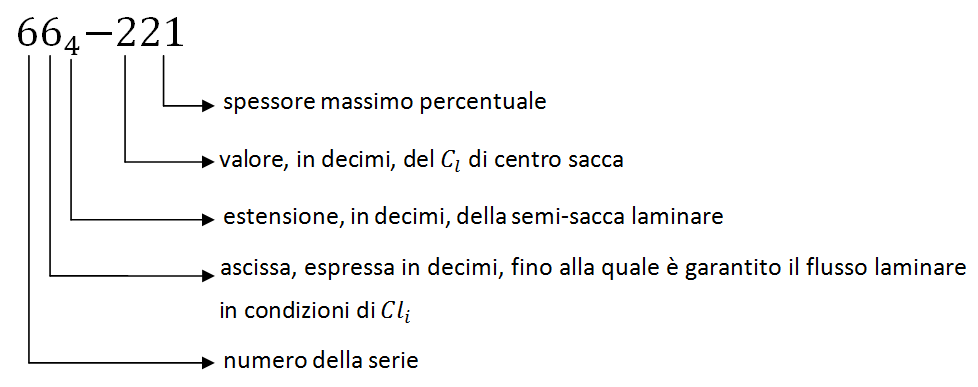
\includegraphics  [ height=6cm] {immagini/laminare.png}
\caption{\footnotesize Significato cifre profilo laminare NACA $66_4-221$ }
\label{fig:lamin}
\end{figure}

\noindent \\

Di seguito saranno svolti sul detto profilo i medesimi studi effettuati nella {\itshape Parte I} relativamente al profilo {\bfseries SELIG 4110}, pertanto, in questa sede, saranno limitate al massimo eventuali spiegazioni non strettamente necessarie.\\
In primo luogo verrà trattata la geometria del profilo, e la relativa costruzione. In seguito verranno ricavate le caratteristiche geometriche dello stesso e i risultati del profilo sottile. Sará poi studiata la soluzione in campo Euleriano incomprimibile a vari $C_l$ significativi, graficandone il coefficiente di pressione e la soluzione in campo viscoso introducendo,quindi, gli effetti del numero di Reynolds.

%\chapter{Geometria del Profilo}

La geometria di un Profilo Sesta Serie NACA Laminare è data in forma tabellare a partire dal profilo simmetrico e dalla linea media standard.\\ I punti di partenza per la disegnazione tecnica del profilo NACA $66_4-221$ sono stati tratti dal  H. ABBOTT (1958) \cite{prof:abbott}.\\ 

\begin{figure}[H]
\centering
\begin {minipage} [c] {.40\textwidth}
\centering\setlength{\captionmargin}{0pt}%
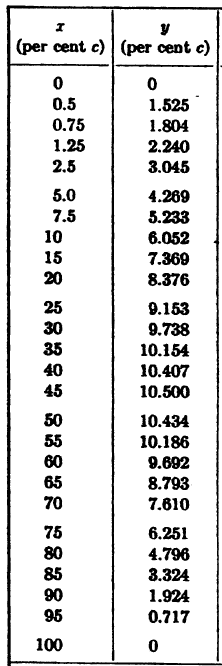
\includegraphics[width=.63\textwidth]{immagini/simmetrico.png}      % 
\caption{Profilo $66_4-021$} %
\end{minipage}
\hspace{13mm}%
\begin {minipage} [c] {.40\textwidth}
\centering\setlength{\captionmargin}{0pt}%
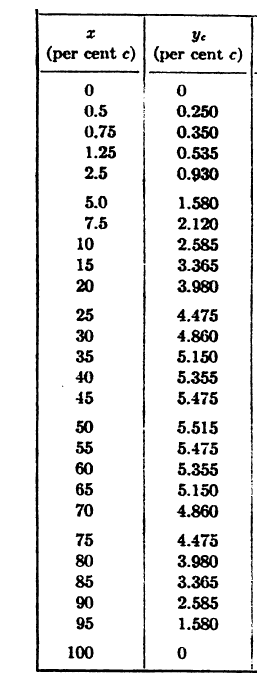
\includegraphics[width=.63\textwidth]{immagini/lineamedia.png}      % 
\caption{Linea media standard} %
\end{minipage}
\end{figure}

\newpage 

\begin{figure} [H]
\centering
\begin{tikzpicture} 
\begin{axis} [ 
xmin=0, 
xmax=1, 
ymin=-0.15,
 ymax=0.15,
 xlabel=$ \frac {x}{c}$, 
ylabel=$ \frac {z}{c}$,
ytick={-0.15,-0.1,-0.05,0,0.05,0.1,0.15},
yticklabels={$-0.15$,$-0.1$,$-0.05$,$0$,$0.05$,$0.1$,$0.15$},
width=13cm,
 height=3.9 cm,
scale only axis,
grid=major] 
\addplot [black,very thick,smooth]
file{immagini/punti_664221_pane.dat};
\addplot [black,very thick,smooth]
file{immagini/lineamedia_NACA664221.dat};
\end{axis}
\end{tikzpicture}
\caption{\footnotesize Profilo  NACA $66_4-221$ }
\end{figure}

\noindent \\

Il disegno tecnico del profilo NACA $66_4-221$ è stato eseguito a partire dai punti del profilo simmetrico NACA $66_4-021$ e di quelli della linea media standard, questi ultimi opportunamente scalati per tener conto del $C_{li}=0.2$. Di seguito sono riportati i disegni necessari per quanto concerne la costruzione del profilo stesso.\\

\begin{figure} [H]
\centering
\begin{tikzpicture} 
\begin{axis} [ 
xmin=0, 
xmax=1, 
ymin=-0.15,
 ymax=0.15,
 xlabel=$ \frac {x}{c}$, 
ylabel=$ \frac {z}{c}$,
ytick={-0.15,-0.1,-0.05,0,0.05,0.1,0.15},
yticklabels={$-0.15$,$-0.1$,$-0.05$,$0$,$0.05$,$0.1$,$0.15$},
width=13cm,
 height=3.9 cm,
scale only axis,
grid=major] 
\addplot [black, mark=*,only marks]
file{immagini/profilo_simmetrico_NACA664021.dat};
\end{axis}
\end{tikzpicture}
\caption{\footnotesize Profilo simmetrico per punti NACA $66_4-021$ }
\end{figure}

\begin{figure} [H]
\centering
\begin{tikzpicture} 
\begin{axis} [ 
xmin=0, 
xmax=1, 
ymin=-0.1,
 ymax=0.1,
 xlabel=$ \frac {x}{c}$, 
ylabel=$ \frac {z}{c}$,
ytick={-0.1,-0.05,0,0.05,0.1},
yticklabels={$-0.1$,$-0.05$,$0$,$0.05$,$0.1$},
width=13cm,
 height=2.6 cm,
scale only axis,
grid=major] 
\addplot [black, mark=*]
file{immagini/lineamedia_NACA664221.dat};
\end{axis}
\end{tikzpicture}
\caption{\footnotesize linea media a=1 $C_{li}=0.2$ }
\end{figure}

\begin{figure} [H]
\centering
\begin{tikzpicture} 
\begin{axis} [ 
xmin=0, 
xmax=1, 
ymin=-0.15,
 ymax=0.15,
 xlabel=$ \frac {x}{c}$, 
ylabel=$ \frac {z}{c}$,
ytick={-0.15,-0.1,-0.05,0,0.05,0.1,0.15},
yticklabels={$-0.15$,$-0.1$,$-0.05$,$0$,$0.05$,$0.1$,$0.15$},
width=13cm,
 height=3.9 cm,
scale only axis,
grid=major] 
\addplot [black, mark=*,only marks]
file{immagini/punti_profilo_664221.dat};
\end{axis}
\end{tikzpicture}
\caption{\footnotesize Profilo per punti NACA $66_4-221$ }
\end{figure}

\begin{figure} [H]
\centering
\begin{tikzpicture} 
\begin{axis} [ 
xmin=0, 
xmax=1, 
ymin=-0.15,
 ymax=0.15,
 xlabel=$ \frac {x}{c}$, 
ylabel=$ \frac {z}{c}$,
ytick={-0.15,-0.1,-0.05,0,0.05,0.1,0.15},
yticklabels={$-0.15$,$-0.1$,$-0.05$,$0$,$0.05$,$0.1$,$0.15$},
width=13cm,
 height=3.9 cm,
scale only axis,
grid=major] 
\addplot [black, mark=*,only marks]
file{immagini/punti_profilo_664221.dat};
\addplot [black,very thick,smooth]
file{immagini/punti_664221_pane.dat};
\addplot [black,very thick,smooth]
file{immagini/lineamedia_NACA664221.dat};
\end{axis}
\end{tikzpicture}
\caption{\footnotesize Confronto punti con interpolante profilo NACA $66_4-221$ }
\end{figure}

\begin{figure} [h!]
\centering
\begin{tikzpicture} 
\begin{axis} [ 
xmin=0.9, 
xmax=1.02, 
ymin=-0.03,
 ymax=0.03,
 xlabel=$ \frac {x}{c}$, 
ylabel=$ \frac {z}{c}$,
%xtick={-0.03,0,0.03,0.06,0.09},
width=13cm,
 height=6.5 cm,
scale only axis,
grid=major] 
\addplot [black,very thick,smooth]
file{immagini/punti_664221_pane.dat};
\end{axis}
\end{tikzpicture}
\caption{\footnotesize Profilo alare NACA $66_4-221$. Zoom del bordo d'uscita }
\end{figure}

\begin{figure} [h!]
\centering
\begin{tikzpicture} 
\begin{axis} [ 
xmin=-0.02, 
xmax=0.05, 
ymin=-0.05,
 ymax=0.05,
 xlabel=$ \frac {x}{c}$, 
ylabel=$ \frac {z}{c}$,
xtick={-0.03,0,0.03,0.06,0.09},
width=6.3cm,
height=9 cm,
scale only axis,
grid=major] 
\addplot [black,very thick,smooth]
file{immagini/punti_664221_pane.dat};
\end{axis}
\end{tikzpicture}
\caption{\footnotesize Profilo alare NACA$66_4-221$. Zoom del bordo d'attacco }
\end{figure}

Tramite xfoil è stata ricavato l'andamento della curvatura del profilo in funzione dell'ascissa curvilinea, riportato nelle figure che seguono.\\

\begin{figure} [H]
\centering
\begin{tikzpicture} 
\begin{axis} [ 
xmin=0, 
xmax=2.02, 
ymin=-2.6,
 ymax=60,
 xlabel=$ \frac {s}{c}$, 
ylabel=$ curvatura$,
width=11cm,
 height=7 cm,
scale only axis,
grid=major] 
\addplot [black,solid,very thick]
file{immagini/curvatura_laminare.dat};
\end{axis}
\end{tikzpicture}
\caption{\footnotesize NACA $66_4221$- Andamento ascissa curvilinea - curvatura }
\end{figure}
\noindent
 \\ \\

\begin{figure} [H]
\centering
\begin{tikzpicture} 
\begin{axis} [ 
xmin=0, 
xmax=2.02, 
ymin=-2.6,
 ymax=2.5,
 xlabel=$ \frac {s}{c}$, 
ylabel=$ curvatura$,
width=11cm,
 height=7 cm,
scale only axis,
grid=major] 
\addplot [black,solid,very thick]
file{immagini/curvatura_laminare.dat};
\end{axis}
\end{tikzpicture}
\caption{\footnotesize  NACA $66_4-221$ -Andamento ascissa curvilinea - curvatura, zoom }
\end{figure}
\noindent
 \\

 Al fine di migliorare la geometria, i punti di ascissa ({\bfseries X}), ordinata({\bfseries Y}) e ascissa curvilinea del profilo ({\bfseries S}),  sono stati importati in MATLAB ed elaborati con un codice in grado di generare delle {\itshape spline} X(S) e Y(S) ed interpolarle al fine di ottenere 100 punti sul dorso e 100 punti sul ventre, alle stesse ascisse.

\begin{figure} [h!]
\centering
\begin{tikzpicture} 
\begin{axis} [ 
xmin=0, 
xmax=2.02, 
ymin=0,
 ymax=1,
 xlabel=$ \frac {s}{c}$, 
ylabel=$ \frac {x}{c}$,
width=12cm,
 height=5.5 cm,
scale only axis,
grid=major] 
\addplot [black,solid,very thick]
file{immagini/acissa_ascissacurvilinea_laminare.dat};
\end{axis}
\end{tikzpicture}
\caption{\footnotesize NACA $66_4-221$ Andamento ascissa curvilinea - ascissa }
\end{figure}


\begin{figure} [h!]
\centering
\begin{tikzpicture} 
\begin{axis} [ 
xmin=0, 
xmax=2.02, 
ymin=-0.1,
 ymax=0.15,
 xlabel=$ \frac {s}{c}$, 
ylabel=$ \frac {z}{c}$,
width=12cm,
 height=6 cm,
scale only axis,
ytick={-0.1,-0.05,0,0.05,0.1,0.15},
yticklabels={$-0.1$,$-0.05$,$0$,$0.05$,$0.1$,$0.15$},
grid=major] 
\addplot [black,solid,very thick]
file{immagini/ordinata_ascissacurvilinea_laminare.dat};
\end{axis}
\end{tikzpicture}
\caption{\footnotesize NACA $66_4-221$ Andamento ascissa curvilinea - ordinata}
\end{figure}
\noindent  \\ 

I punti del profilo sono stati importati sul software CAD CATIA V5 per rappresentare l’ala infinita, con profilo costante, di elevato allungamento.\\

\begin{figure} [h!]
\centering
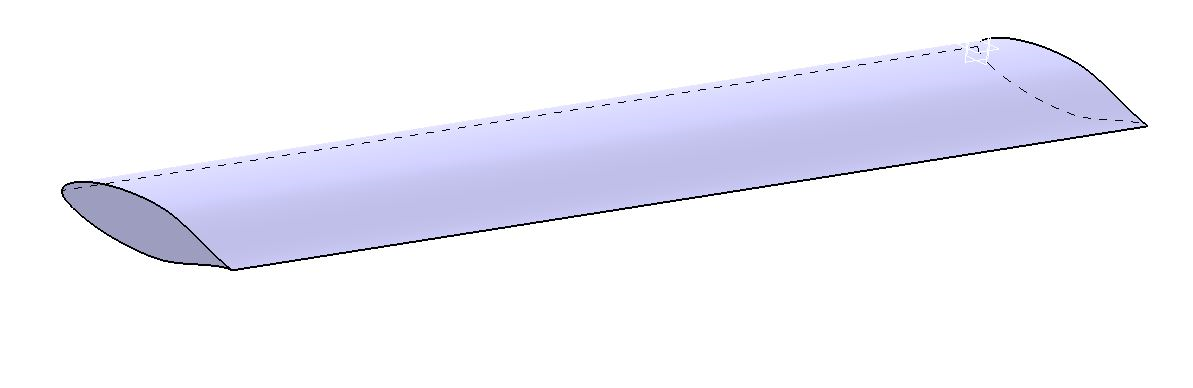
\includegraphics  [ height=5cm] {immagini/fig11.png}
\caption{\footnotesize Ala infinita, profilo costante NACA $66_4-221$, rendering in CATIA V5}
\end{figure}


%\chapter{Aerodinamica non viscosa incomprimibile}

Nel seguente capitolo verranno esposti i risultati ottenuti circa le caratteristiche del profilo in termini di retta di portanza, angolo d’attacco ideale e di portanza nulla e coefficiente di momento focale. Infine verranno graficate le distribuzioni del coefficiente di pressione al variare del $C_l $.\\
Saranno di seguito rappresentati solo i risultati grafici in quanto le considerazioni relative alla costruzione di tali grafici sono già state fatte nella parte I.

\section{ Andamento di portanza e momento}

\begin{figure} [h!]
\centering
\begin{tikzpicture} 
\begin{axis} [ 
xmin=-10, 
xmax=10, 
ymin=-1,
ymax=1.6,
xlabel=$ \alpha$, 
ylabel=$ C_l $,
ytick={-1,-0.8,-0.6,-0.4,-0.2,0,0.2,0.4,0.6,0.8,1,1.2,1.4,1.6},
width=10cm,
height=7.5cm,
scale only axis,
grid=major] 
\addplot [black,very thick]
file{immagini/cla_laminare.dat};
\end{axis}
\end{tikzpicture}
\caption{\footnotesize Retta di portanza del profilo alare NACA $66_4-221$, soluzione euleriana incomprimibile }
\end{figure}
\noindent
\\ 

\begin{figure} [h!]
\centering
\begin{tikzpicture} 
\begin{axis} [ 
xmin=-10, 
xmax=10, 
ymin=-0.5,
ymax=0.5,
xlabel=$ \alpha$, 
ylabel=$ C_m$,
ytick={-0.5,-0.4,-0.3,-0.2,-0.1,0,0.1,0.2,0.3,0.4,0.5},
width=10cm,
height=6.5 cm,
scale only axis,
grid=major] 
\addplot [black,very thick]
file{immagini/cm_laminare.dat};
\end{axis}
\end{tikzpicture}
\caption{\footnotesize Curva di momento del profilo alare NACA $66_4-221$, soluzione euleriana incomprimibile, polo ad $ \frac {x}{c}$ =$ \frac {1}{4}$ }
\end{figure}

\section{Centro di Pressione}

Il centro di pressione è quel punto in cui si puó ritenere applicata la risultante delle forze fluidodinamiche agenti sul profilo.\\

\begin{figure} [H]
\centering
\begin{tikzpicture}
\begin{axis}[
xmin=-12,
xmax=12,
ymin=-4,
ymax=4,
xlabel=${\alpha}$,
ylabel=$\frac{x_{cp}}{c}$,
width=9cm,
height=6.5cm,
scale only axis,
grid=major]
\addplot[black, very thick]
file{immagini/xcp1_lam.dat};
\addplot[black, very thick]
file{immagini/xcp2_lam.dat};
\end{axis}
\end{tikzpicture}
\caption{\footnotesize Profilo S4110, Andamento dell'ascissa del Centro di Pressione al variare di ${\alpha}$ }\label{fig:cp}
\end{figure}


\section{Risultati della Teoria del Profilo Sottile}

Sono stati calcolati i coefficienti di Fourier dello sviluppo in serie della derivata della linea media ottenendo i seguenti risultati


\begin {itemize}
\item ${\alpha}_i=c_0=-0.0215^\circ$
\item ${\alpha}_{zl}=\frac {c_1}{2}-c_0=-1.69^\circ$
\item $C_{m\frac {c}{4}}=-\frac {{\pi}}{4}(c_1-c_2)=-0.0439$
\end{itemize}

\noindent \\ 
Ottenuto un $c_{l{\alpha}} = 7.16 rad^{-1}$  è possibile ricavare $ k=0.665$

\noindent \\
\section{Coefficiente di Pressione}

Di seguito sono riportati gli andamenti del coefficiente di pressione del profilo alare in studio, nell’ ipotesi di campo Euleriano incomprimibile, in funzione dell’ascissa adimensionalizzata rispetto alla corda a vari $C_l$ di particolare interesse per questo profilo laminare.


\begin{figure} [h!]
\centering
\begin{tikzpicture} 
\begin{axis} [ 
xmin=0, 
xmax=1, 
ymin=-1,
ymax=1,
xlabel=$\frac{x}{c}$, 
ylabel=$C_p$ ,
 y dir=reverse,
width=12cm,
height=7 cm,
scale only axis,
grid=major] 
\addplot [black,very thick, smooth]
file{immagini/CLMENO02.dat};
\end{axis}
\end{tikzpicture}
\caption{\footnotesize NACA $66_4-221$, distribuzione del Coefficiente di Pressione $C_l=-0.2$ (estremo inferiore sacca laminare). Soluzione Euleriana incomprimibile }
\end{figure}

Si noti come cambia notevolmente il comportamento del profilo in sacca e fuori la sacca laminare. Per un $C_l$ che non appartiene alla zona della sacca laminare, si ha un picco sul grafico del Cp mentre per l'intervallo di $C_l$ di sacca si ha assenza di picchi di espansione al bordo d'attacco il che assicura un gradiente di pressione favorevole con un esteso deflusso laminare.

\begin{figure} [H]
\centering
\begin{tikzpicture} 
\begin{axis} [ 
xmin=0, 
xmax=1, 
ymin=-1,
ymax=1,
xlabel=$\frac{x}{c}$, 
ylabel=$C_p$ ,
 y dir=reverse,
width=12cm,
height=7 cm,
scale only axis,
grid=major] 
\addplot [black,very thick,smooth]
file{immagini/cl_0_laminare.dat};
\end{axis}
\end{tikzpicture}
\caption{\footnotesize NACA $66_4-221$, distribuzione del Coefficiente di Pressione $C_l=0$. Soluzione Euleriana incomprimibile }
\end{figure}


\begin{figure} [h!]
\centering
\begin{tikzpicture} 
\begin{axis} [ 
xmin=0, 
xmax=1, 
ymin=-1,
ymax=1,
xlabel=$\frac{x}{c}$, 
ylabel=$C_p$ ,
 y dir=reverse,
width=12cm,
height=7 cm,
scale only axis,
grid=major] 
\addplot [black,very thick, smooth]
file{immagini/cl_0.2_laminare.dat};
\end{axis}
\end{tikzpicture}
\caption{\footnotesize NACA $66_4-221$, distribuzione del Coefficiente di Pressione $C_l=0.2$ (centro sacca). Soluzione Euleriana incomprimibile }
\end{figure}




\begin{figure} 
\centering
\begin{tikzpicture} 
\begin{axis} [ 
xmin=0, 
xmax=1, 
ymin=-1.5,
ymax=1,
xlabel=$\frac{x}{c}$, 
ylabel=$C_p$ ,
 y dir=reverse,
width=12cm,
height=7 cm,
scale only axis,
grid=major] 
\addplot [black,very thick, smooth]
file{immagini/cl_0.6_laminare.dat};
\end{axis}
\end{tikzpicture}
\caption{\footnotesize NACA $66_4-221$, distribuzione del Coefficiente di Pressione $C_l=0.6$ (estremo superiore sacca laminare). Soluzione Euleriana incomprimibile }
\end{figure}

\begin{figure} 
\centering
\begin{tikzpicture} 
\begin{axis} [ 
xmin=0, 
xmax=1, 
ymin=-3,
ymax=1,
xlabel=$\frac{x}{c}$, 
ylabel=$C_p$ ,
 y dir=reverse,
width=12cm,
height=7 cm,
scale only axis,
grid=major] 
\addplot [black,very thick]
file{immagini/cl_1_laminare.dat};
\end{axis}
\end{tikzpicture}
\caption{\footnotesize NACA $66_4-221$, distribuzione del Coefficiente di Pressione $C_l=1$ . Soluzione Euleriana incomprimibile }
\end{figure}

\noindent \\


%\chapter{Effetti della Comprimibilità}

Tramite XFOIL è stato ricavato il valore $M_{\infty crit}$=0.626 in corrispondenza di $C_l$=$C_{l_{id}}$=0.2. \\
Di seguito saranno rappresentati graficamente la variazione del $M_{\infty crit}$ con il $C_L$ e gli effetti della comprimibilità lineare sul Cp e sulla retta di portanza.\\ 

\begin{figure} [H]
\centering
\begin{tikzpicture} 
\begin{axis} [ 
xmin=-1.5, 
xmax=1.5, 
ymin=0.2,
ymax=0.8,
xlabel=$C_l$, 
ylabel=$M_{\infty}$ ,
width=10cm,
height=6 cm,
scale only axis,
grid=major] 
\addplot [black,very thick]
file{immagini/critico_laminare.dat};
\end{axis}
\end{tikzpicture}
\caption{\footnotesize Andamento del $ M_{\infty crit} $  al variare del Coefficiente di Portanza, profilo NACA $66_4-221$}
\end{figure}
\noindent \\


\begin{figure} [h!]
\centering
\begin{tikzpicture} 
\begin{axis} [ 
xmin=0, 
xmax=1, 
ymin=-1,
ymax=1.5,
xlabel=$\frac{x}{c}$, 
ylabel=$C_p$ ,
 y dir=reverse,
width=12cm,
height=7 cm,
scale only axis,
grid=major] 
\addplot [black,very thin, smooth]
file{immagini/AAAAM0.dat};
\addplot [black,thick, smooth]
file{immagini/AAAM02.dat};
\addplot [black,ultra thick, smooth]
file{immagini/AAA04.dat};
\legend {$M_{\infty}=0$,$M_{\infty}=0.2$,$M_{\infty}=0.4$}
\end{axis}
\end{tikzpicture}
\caption{\footnotesize NACA $66_4-221$, confronto del Coefficiente di Pressione per $C_l=0.2$ (centro sacca) al variare del numero di Mach}
\end{figure}


Come si puó notare per effetto della comprimibilità cambierà la distribuzione del Coefficiente di pressione lungo il profilo. In particolare, all’aumentare del numero di Mach, le zone espanse espandono di più, e quelle compresse comprimono di più.\\
Successivamente tramite XFOIL sono stati studiati gli effetti della comprimibilitá lineare sulla retta di portanza, quindi è stato valutato ció tramite la similitudine di Karman e Tsein.


\begin{figure} [h!]
\centering
\begin{tikzpicture} 
\begin{axis} [ 
legend style={at={(0.3,0.98)}},
xmin=-12, 
xmax=12, 
ymin=-1,
ymax=1.6,
xlabel=$ \alpha$, 
ylabel=$ C_l $,
%ytick={-1,-0.8,-0.6,-0.4,-0.2,0,0.2,0.4,0.6,0.8,1,1.2,1.4,1.6},
width=10cm,
height=7.5cm,
scale only axis,
grid=major] 
\addplot [black,very thin]
file{immagini/M0.dat};
\addplot [black, thick]
file{immagini/M2.dat};
\addplot [black,ultra thick]
file{immagini/M4.dat};
\legend {$M_{\infty}=0$,$M_{\infty}=0.2$,$M_{\infty}=0.4$}
\end{axis}
\end{tikzpicture}
\caption{\footnotesize Confronto della retta di portanza del profilo alare NACA $66_4-221$ al variare del numero di Mach }
\end{figure}
\noindent
\\ 
%\chapter{Effetti viscosi}

In questo capitolo sarà studiata l’aerodinamica del profilo alare Sesta Serie NACA Laminare $66_4-221$ a diversi assetti.\\ In primo luogo saranno evidenziati gli effetti della viscosità sulla curva di portanza e sulla polare, ponendo particolare attenzione al comportamento della zona della sacca laminare. In seguito si studierà la variazione della distribuzione del Coefficiente di Pressione con il numero di Reynolds ad assetti anche non piccoli.  

\section{Curva di Portanza e polare }

I valori dell' $ {\alpha}_{stall}$ e del $C_{l_{max}}$ sono i seguenti \\


\begin {itemize}
\item $Re=3*10^6$ ${\to}$ $ {\alpha}_{stall}=22^\circ$  ${\to}$ $C_{l_{max}}=1.47$
\item $Re=7*10^6$ ${\to}$ $ {\alpha}_{stall}=23^\circ$  ${\to}$ $C_{l_{max}}=1.60$
\item $Re=1*10^7$ ${\to}$ $ {\alpha}_{stall}=25^\circ$  ${\to}$ $C_{l_{max}}=1.65$
\end{itemize}

\noindent \\ \\
Nel grafico della polare del profilo si può notare la presenza di una sacca laminare intorno al valore del $C_{l_i}$ la cui estensione varia al variare del numero di Reynolds.\\ Per $ Re=3*10^6$ l’estensione della semisacca è di poco superiore a 0.4, valore designato nella sigla del profilo. Per numeri di Reynolds minori la sacca diventa più ampia, per numeri di Reynolds maggiori, la sacca riduce la propria estensione e arretra con una conseguente diminuzione del minimo coefficiente di resistenza.

\begin{figure} [H]
\centering
\begin{tikzpicture} 
\begin{axis} [ 
legend style={at={(0.3,0.98)}},
xmin=-25, 
xmax=25, 
ymin=-1.8,
ymax=1.8,
xlabel=${\alpha}$,
ylabel=$C_l$ ,
width=12cm,
height=19 cm,
scale only axis,
grid=major] 
\addplot [black, smooth,mark=*]
file{immagini/3_10_6_lam.dat};
\addplot [black,smooth,mark=diamond*]
file{immagini/7_10_6_lam.dat};
\addplot [black, smooth,mark=star]
file{immagini/1_10_7_lam.dat};
\legend {$Re=3*10^6$,$Re=7*10^6$,$Re=1*10^7$}
\end{axis}
\end{tikzpicture} 
\caption{\footnotesize Confronto delle curve di Portanza del profilo {\bfseries NACA $66_4-221$} al variare del numero di Reynolds }
\end{figure}


\begin{figure} [H]
\centering
\begin{tikzpicture} 
\begin{axis} [ 
legend style={at={(0.98,0.35)}},
xmin=0, 
xmax=0.07, 
ymin=-1.6,
ymax=1.8,
xlabel=$C_d$,
ylabel=$C_l$ ,
xtick={0.01,0.02,0.03,0.04,0.05,0.06,0.07},
xticklabels={$0.01$,$0.02$,$0.03$,$0.04$,$0.05$,$0.06$,$0.07$},
width=11cm,
height=11cm,
scale only axis,
grid=major] 
\addplot [black, smooth,mark=*]
file{immagini/cd_cl_3_10_6_laminare.dat};
\addplot [black, smooth,mark=diamond*]
file{immagini/cd_cl_7_10_6_laminare.dat};
\addplot [black, smooth,mark=star]
file{immagini/cd_cl_1_10_7_laminare.dat};
\legend {$Re=3*10^6$,$Re=7*10^6$,$Re=1*10^7$}
\end{axis}
\end{tikzpicture}
\caption{\footnotesize Confronto delle Polari del profilo {\bfseries NACA $66_4-221$} al variare del numero di Reynolds }
\end{figure}

\begin{figure} [H]
\centering
\begin{tikzpicture} 
\begin{axis} [ 
legend style={at={(0.98,0.60)}},
xmin=0.002, 
xmax=0.01, 
ymin=-0.4,
ymax=0.8,
xlabel=$C_d$,
ylabel=$C_l$ ,
xtick={0.002,0.003,0.004,0.005,0.006,0.007,0.008,0.009,0.01},
%xticklabels={$0.01$,$0.02$,$0.03$,$0.04$,$0.05$,$0.06$,$0.07$,$0.08$,$0.09$,$0.1$},
width=7cm,
height=6cm,
scale only axis,
grid=major] 
\addplot [black, smooth,mark=*]
file{immagini/cd_cl_3_10_6_laminare.dat};
\addplot [black, smooth,mark=diamond*]
file{immagini/cd_cl_7_10_6_laminare.dat};
\addplot [black, smooth,mark=star]
file{immagini/cd_cl_1_10_7_laminare.dat};
\legend {$Re=3*10^6$,$Re=7*10^6$,$Re=1*10^7$}
\end{axis}
\end{tikzpicture}
\caption{\footnotesize Confronto delle Polari del profilo {\bfseries NACA $66_4-221$} al variare del numero di Reynolds, zoom della sacca laminare }
\end{figure}


\section{Coefficiente di pressione al variare del numero di Reynolds }

\begin{figure} [H]
\centering
\begin{tikzpicture} 
\begin{axis} [ 
xmin=0, 
xmax=1, 
ymin=-1.5,
ymax=1,
xlabel=$\frac{x}{c}$, 
ylabel=$C_p$ ,
 y dir=reverse,
width=12cm,
height=5.5 cm,
scale only axis,
grid=major] 
\addplot [black,very thin]
file{immagini/cp3106.dat};
\addplot [black,thick]
file{immagini/cp_7_10_6_cl_02_laminare.dat};
\addplot [black,ultra thick]
file{immagini/cp_1_10_7_cl_02_laminare.dat};
\legend {$Re=3*10^6$,$Re=7*10^6 $,$Re=1*10^7$}
\end{axis}
\end{tikzpicture}
\caption{\footnotesize Profilo NACA $66_4-221$, confronto del Coefficiente di Pressione per $C_l=C_{l_{id}}=0.1$ al variare del numero di Reynolds}
\end{figure}

\begin{figure} [H]
\centering
\begin{tikzpicture} 
\begin{axis} [ 
xmin=0, 
xmax=1, 
ymin=-5,
ymax=1,
xlabel=$\frac{x}{c}$, 
ylabel=$C_p$ ,
 y dir=reverse,
width=12cm,
height=5.5 cm,
scale only axis,
grid=major] 
\addplot [black,very thin]
file{immagini/cl1_3_10_6_lam.dat};
\addplot [black,thick]
file{immagini/cl_1_7_10_6_lam.dat};
\addplot [black,ultra thick]
file{immagini/cl_1_1_10_7_lam.dat};
\legend {$Re=3*10^6$,$Re=7*10^6 $,$Re=1*10^7$}
\end{axis}
\end{tikzpicture}
\caption{\footnotesize Profilo NACA $66_4-221$, confronto del Coefficiente di Pressione per $C_l=1$ al variare del numero di Reynolds}
\end{figure}



\section{Stallo}
Per vedere il tipo di stallo cui va incontro il profilo si è applicato il criterio semiempirico di Thain e Gault considerando i numeri di Reynolds scelti e lo spessore percentuale all'$1.25 \%$ della corda che assume un valore di $2.47 \%$ definendo così uno stallo da separazione al bordo d'uscita.

%
%
\part {L' Aerodinamica del velivolo Airbus~A340-200}
% !TeX program = PdfLaTeX
% !TeX root = ../../Elaborati_Aerodinamica_Bruno_Spoti.tex

\chapter{Introduzione}
In questa terza parte ci si prefigge di caratterizzare l’aerodinamica del velivolo di linea quadrimotore \emph{Airbus A340-200}. \cite{author:airbusA340}.\\
%Preliminarmente sono stati reperiti i dati di principale interesse.
\begin {figure} [h!]
\centering
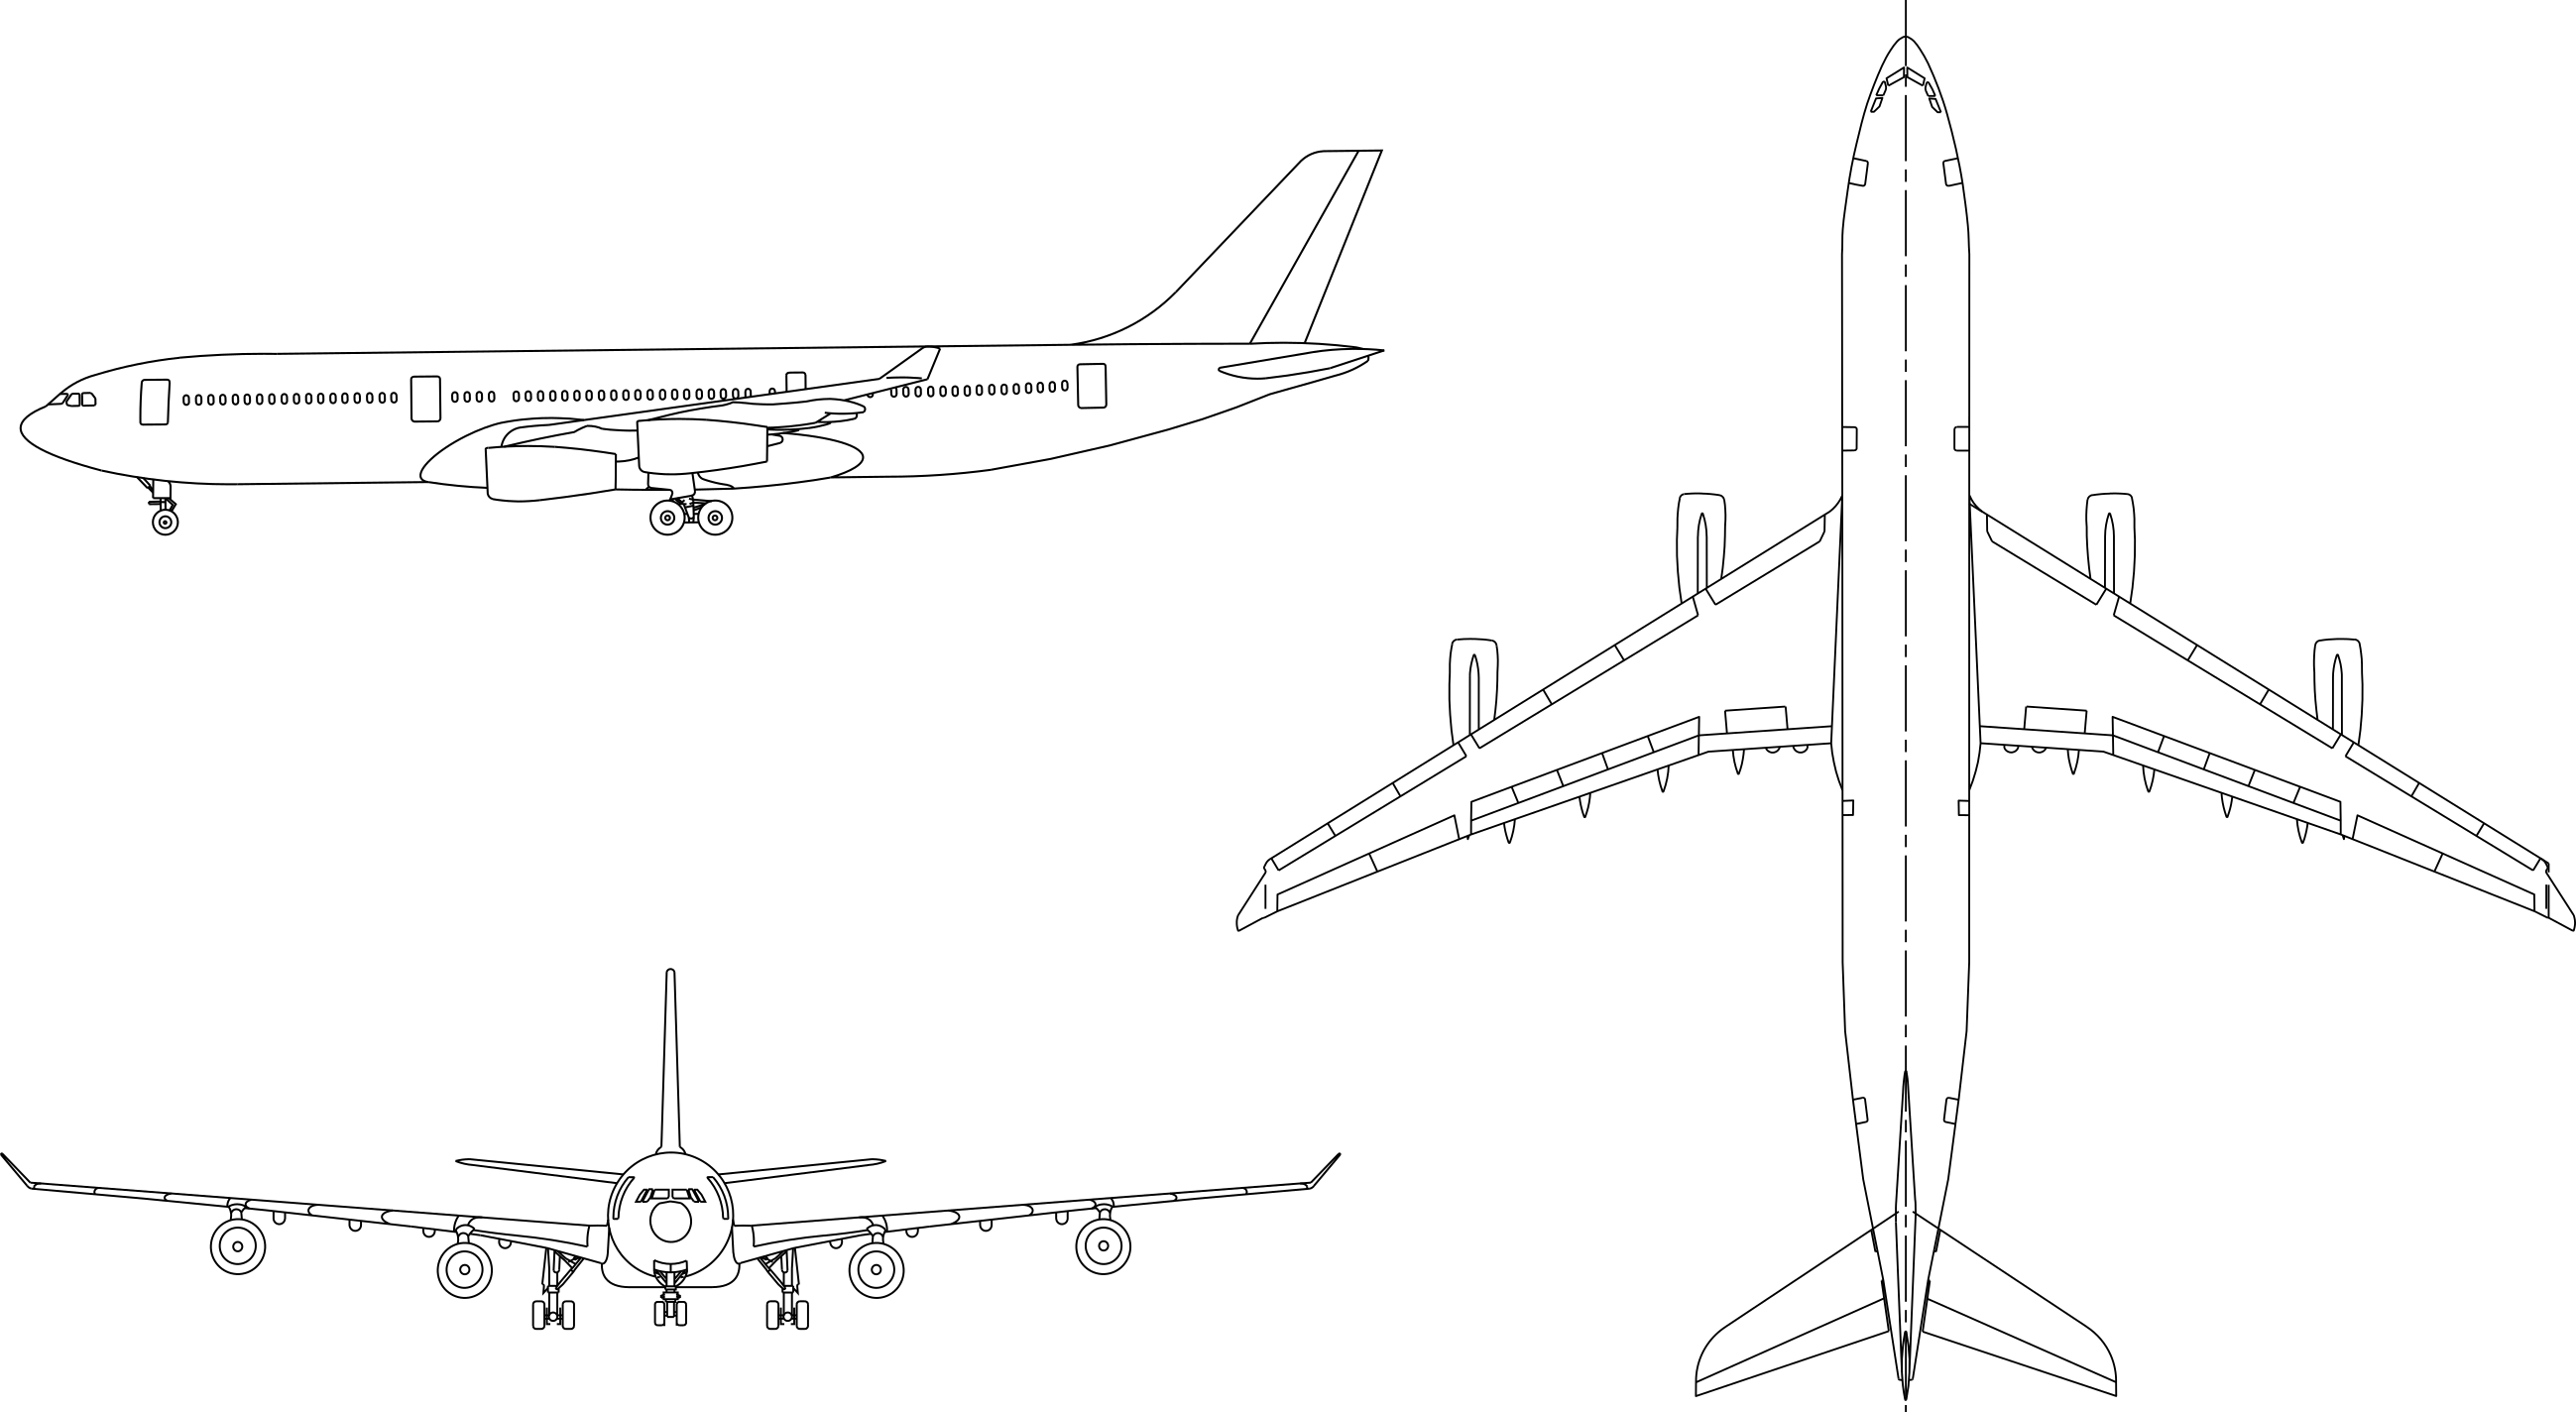
\includegraphics[width= \textwidth ]{images/fileImg/Parte_3-Aerodinamica_Velivolo_A340-200/tritticoA340-200.png}
\caption{\footnotesize Trittico Airbus A340-200}
\label {fig:trittico}
\end {figure}

Nella tabella~\ref{tabV1} e~\vref{tabV2}  sono elencanti i dati geometrici d'interesse del velivolo. \cite{author:airbusA340} \cite{author:Jane}  \\ \\ 


\begin{table} [!h]\centering \rowcolors{1}{}{grigio_chiaro}
\begin{tabular}{l c c}
\toprule
\multicolumn{3}{c}{\emph{Dati Geometrici}} \\ 
\midrule
Apertura Alare 		& $b$  					&   	$60.30 \si{m} $ 		\\
Superficie Alare & $S_\mathrm{w}$  		&  		$361.6 \si{m^2} $ 		\\
Allungamento alare & $\AR$ 				& 	    $10.56$ 				\\
Corda alla radice & \croot	&  	$10.6 \si{m}$   \\
Corda all'estremità & \ct							&  		$2.57 \si{m}$ 	    \\
Corda alla sezione di \emph{kink} & \ck							&  		$7.20 \si{m}$ 	    \\
%Fattore di Oswald & $e$	   				& 	    $0.75 $ 				\\
Angolo di freccia al bordo d'attacco & $\Lambda_{le}$ & $32.2^\circ $  \\ 
Angolo diedro dell'ala  & $\Gamma_\mathrm{W}$ & $4.56^\circ $ \\
\midrule
Lunghezza totale  & $L$  					&   	$59.42 \si{m} $ 		\\
Altezza totale & $H$  					&   	$16.84 \si{m} $ 		\\
Massimo diametro della fusoliera & \Dfmax  					&   	$5.64 \si{m} $ \\
Apertura piano di coda orizzontale  &\bHtail & $ 19.41\si{m} $		\\ 

	
\bottomrule
\end{tabular}
\caption {\footnotesize Dati geometrici principali del velivolo Airbus A340-200}
\label{tabV1}
\end{table}

\begin{table} [!h]\centering \rowcolors{1}{}{grigio_chiaro}
	\begin{tabular}{l c c}
		\toprule
		\multicolumn{3}{c}{\emph{Pesi e prestazioni}} \\ 
		\midrule
		Peso a vuoto operativo (OWE) & \WOE & 129500 \si{kg} \\
		Massimo carico pagante & \WPLmax & 45530 \si{kg} \\
		Peso massimo al decollo configurazione base (MTOW)   &\MTOW & 253500 \si{kg} \\
		Peso massimo al'atterraggio    &\WLmax & 181000 \si{kg} \\
		Peso massimo senza carburante    &\Wzfmax & 169000 \si{kg} \\
		Carico alare massimo   &\WoverSmax & 760.5 \si{kg/m^2} \\
		\midrule		
		Numero di Mach massimo operativo & \Mmo & 0.86 \\
		Velocità massima operativa (IAS)  & \Vmo 	&  	$661 \si{km/h} $ 	\\
		Mach di crociera & \Mc &  	$0.82 $ 	\\
		Velocità di crociera & \Vc &  	$630 \si{km/h}$ 	\\
		Velocità di stallo {\itshape full flap} (267000kg, \emph{wheels up})	 & \Vsf 	&  	$247 \si{km/h} $  	\\
		Velocità di stallo {\itshape clean configuration}   & \Vsc&  $299 \si{km/h} $	\\
    	Quota massima certificata & \hmax & 12525 \si{m}\\
		Distanza di decollo	(S/L, MTOW, ISA +15°C) &	\TOFL & 3017 \si{meter}  \\
		Autonimia di distanza con 239 passeggeri &	$R$ & 14816 \si{km}  \\
		\bottomrule
\end{tabular}
	\caption {\footnotesize Pesi e prestazioni caratteristiche del velivolo Airbus A340-200}
	\label{tabV2}
\end{table}

%\begin{table} [!h]
%
%\centering
%\begin {tabular} {lp{6cm} l}
%{\bfseries Dato }  & & { \bfseries Valore} \\ 
%\hline \hline
%Velocità di crociera {\bfseries $V_c$}  & &  $59.16 m/s $ \\
%\hline
%Velocità massima {\bfseries $V_{max}$}  & &   $64.30 m/s $ \\
%\hline
%Velocità di stallo {\itshape full flap} {\bfseries $V_{sf}$} & & $23.15  m/s$ \\
%\hline
%Velocità di stallo {\itshape clean configuration} {\bfseries $V_{sc}$} & & $28.30 m/s$ \\
%\hline
%Peso massimo al decollo {\bfseries $W_{TO_{max}}$} & & $700 Kg $ \\
%\hline
%Peso a vuoto {\bfseries $W_{OE}$} & & $340 Kg $ \\
%\hline
%Massimo peso {\itshape payload} {\bfseries $W_{PL}$} & & $370 Kg $ \\
%\hline
%\end{tabular}
%\caption {Pesi e velocità caratteristiche del velivolo Airbus A340-200}
%\label{tabV2}
%\end{table}
%
%\noindent \\ \\ \\ \\
%
%
%\begin{table} [!h]
%\caption {Quote e densità}
%\centering
%\begin {tabular} {lp{5cm} l}
%{\bfseries Dato }  & & { \bfseries Valore} \\ 
%\hline \hline
%Quota di tangenza {\itshape Service Ceiling}  & &  $ 4570 m $ \\
%\hline
%Densità al livello del mare  {\bfseries ${\rho}_{SL}$}  & & $1.225  Kg/m^3$ \\
%\hline
%Densità alla quota di tangenza  {\bfseries ${\rho}_{C}$}  & & $0.66945  Kg/m^3$ \\
%\hline
%\end{tabular}
%\label{tab:tabellaquote}
%\end{table}

Inoltre tramite il \emph{software} CATIA V5-6R2017 è stato realizzato il CAD dell'ala prolungandone i bordi di attacco e di uscita nella regione della fusoliera fino al piano di simmetria e il CAD del velivolo completo senza superfici mobili come si vede nelle figure~\vref{fig:V2} e~\vref{fig:V3}. 
\begin {figure} [h!]
\centering
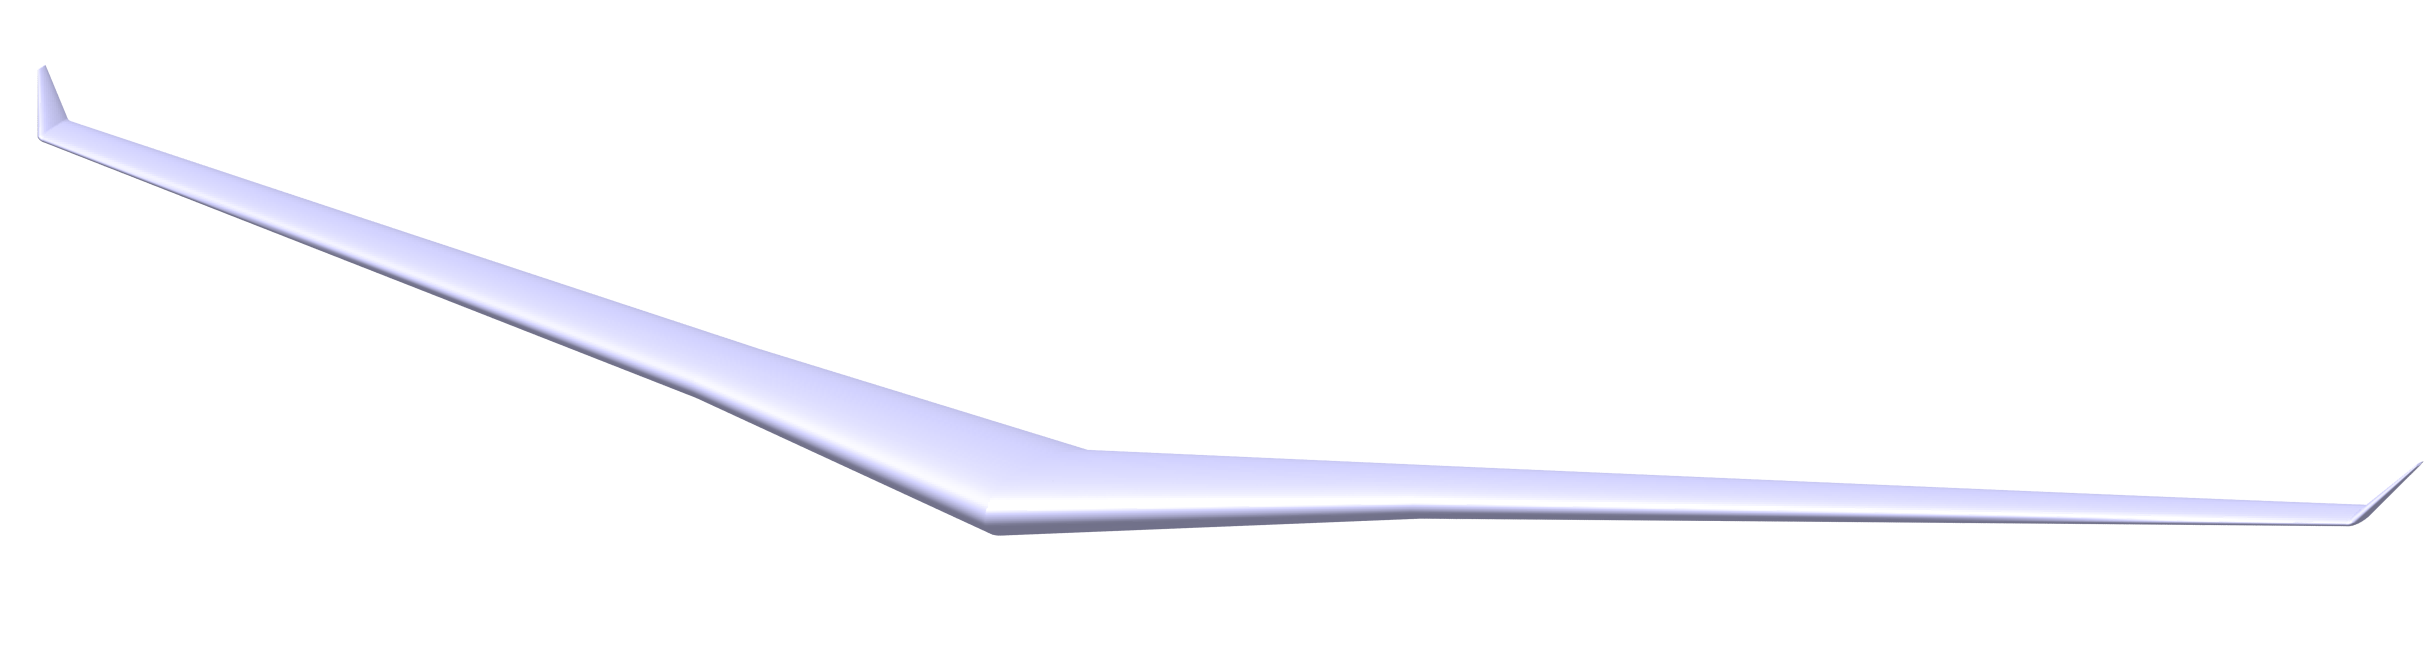
\includegraphics[width= \textwidth ]{images/fileImg/Parte_3-Aerodinamica_Velivolo_A340-200/CadAlaAirbusA340-200.png}
\caption{\footnotesize \emph{Rendering} CAD ala Airbus A340-200. CATIA V5-6R2017}
\label {fig:V2}
\end {figure}

\begin {figure} [h!]
\centering
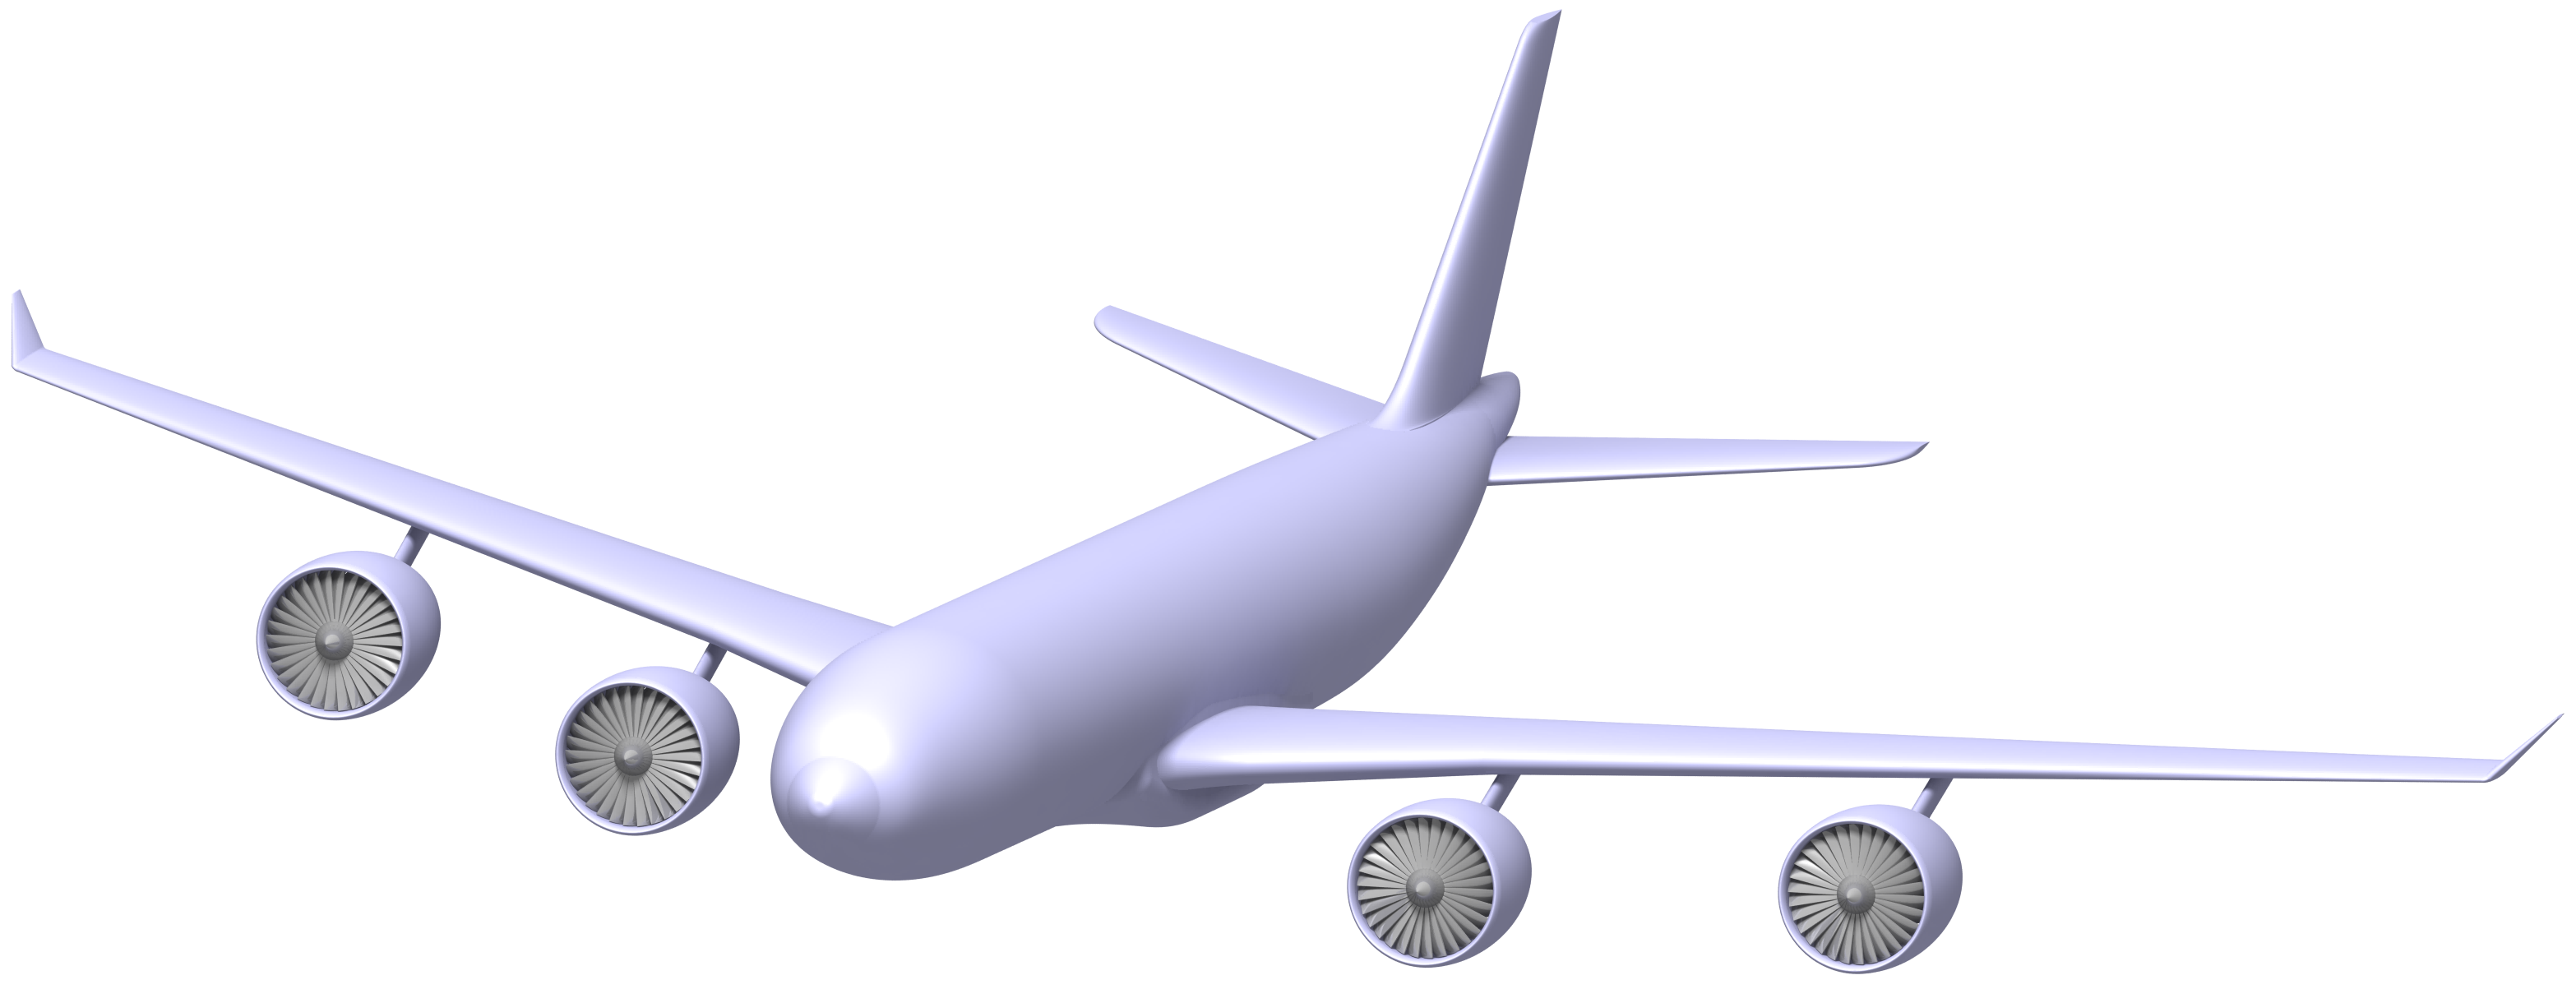
\includegraphics[width= \textwidth ]{images/fileImg/Parte_3-Aerodinamica_Velivolo_A340-200/RenderingA340-200.png}
\caption{\footnotesize \emph{Rendering} CAD velivolo Airbus A340-200. CATIA V5-6R2017}
\label {fig:V3}
\end {figure}




%\input{Teoria_globale_velivolo}o_
%\chapter{Carico lungo l'ala: il Metodo di Schrenk}

Il metodo ingegneristico di Schrenk è un metodo semiempirico che consente il calcolo del carico aerodinamico lungo un'ala dritta nell’ipotesi di assenza di fenomeni viscosi a basse velocità.\\
Tale metodo ha il vantaggio di consentire una valutazione piuttosto veloce ed accettabilmente accurata del carico, molto utile in sede di progetto preliminare.\\
\\
Di seguito, in primo luogo, sarà costruito geometricamente il carico lungo la semiala, e in seguito verranno calcolati il carico basico e quello addizionale per poi ottenere il carico totale lungo l’ala. Infine, con i risultati ottenuti, si valuterà il $C_{l(y)}$ lungo l’ala.

\section{Considerazioni preliminari}

Il profilo utilizzato per l’ala rettangolare, a spessore  e corda costante lungo l’ apertura, è un {\bfseries NACA 4412} \cite{prof:jane} con :

\begin {center}
$C_{l_{\alpha}}=0.1170 deg^{-1}=6.704 rad^{-1}$
\end{center}

il $C_{L{\alpha}}$ dell'ala finita sará calcolato con la seguente formula \\

\begin{equation}
\label{eqn:gt}
C_{L_{\alpha}}=\frac {C_{l_{\alpha}}}{{\pi}{\AR}e}
\end{equation}


da cui si ottiene:\\ 

\begin {center}
$C_{L_{\alpha}}=4.746 rad^{-1}=0.08283 deg^{-1}$
\end{center}


Si suppone uno svergolamento di $-3^\circ $ alle estremità, con una variazione lineare di quest'ultimo.\\
Sará utilizzato un asse lungo l'apertura normalizzato rispetto $\frac{b}{2}$, indicato con $\eta$.\\

Il carico aerodinamico totale che agisce sull’ala può essere scomposto nella somma di due contributi:

\begin {itemize}
\item Carico Addizionale: legato alla portanza dell’ala non svergolata,
\item Carico Basico: dipendente esclusivamente dallo svergolamento.
\end{itemize}

\begin{equation}
\label{eqn:carico}
{\gamma}(y)={\gamma}_a(y)+ {\gamma}_b(y)
\end{equation}

Di seguito saranno valutati questi due termini.


\section{Carico Addizionale}

L'ipotesi fondamentale del metodo di Schrenk è quella di valutare il carico addizionale lungo l’apertura come media tra la distribuzione delle corde dell’ala e la distribuzione di corde dell’{\itshape Ala Ellittica Equivalente}, ossia un’ala con forma in pianta ellittica, con stessa apertura e stessa superficie di quella della quale si vuole calcolare il carico.\\
Per graficare questo carico su un piano $c-y$ occorre rappresentare la distribuzione delle corde dell'ala del J450 e quella dell'ala ellittica equivalente, dopo averne calcolato la corda di radice, essendo nulla quella all'estremità. 

\begin{figure} [h]
\centering
\begin{tikzpicture} 
\begin{axis} [ 
xmin=0, 
xmax=5, 
ymin=0,
ymax=2,
xlabel=$y$, 
ylabel=$c$ ,
width=14cm,
height=5.6cm,
scale only axis,
grid=major] 
\addplot [black, thick]
file{immagini/rett.dat};
\addplot [black, thick, dashed, smooth]
file{immagini/ell.dat};
\addplot [black, thick, dashdotdotted,smooth]
file{immagini/ellnew.dat};
\legend {distribuzione corde,ala ellittica equivalente, carico}
\end{axis}
\end{tikzpicture}
\caption{\footnotesize Velivolo Jabiru J450, costruzione del carico addizionale con il metodo Schrenk}
\end{figure}

\noindent \\

Per un ampio intervallo di assetti, il carico addizionale risulta proporzionale al $C_L$, per cui si ha 

\begin{equation}
\label{eqn:one}
\gamma_a(y)=C_L \gamma_{a1}(y)
\end{equation}

Dalle \ref{eqn:one}, \ref{eqn:two}, \ref{eqn:tree}


\begin{equation}
\label{eqn:two}
\gamma_{a1}(\eta)=\frac{cC_{l_a}}{2b}=\frac{c+c_{ell}}{4b}
\end{equation}

\noindent \\

\begin{equation}
\label{eqn:tree}
cC_{la1}=\frac{c(y)+c_{ell}(y)}{2}
\end{equation}

Si ricava la distribuzione del carico addizionale riportata nel grafico che segue


\begin{figure} [h]
\centering
\begin{tikzpicture} 
\begin{axis} [ 
xmin=0, 
xmax=1, 
ymin=0,
ymax=0.03,
xlabel=$\eta$, 
ylabel=$\gamma_a$ ,
width=14cm,
height=7cm,
scale only axis,
grid=major] 
\addplot [black,very thick,smooth]
file{immagini/gammaadd.dat};
\end{axis}
\end{tikzpicture}
\caption{\footnotesize Velivolo Jabiru J450, carico addizionale lungo la semiala per {\bfseries $C_L=0.3$}}
\end{figure}


\section{Carico Basico}

Il metodo di Schrenk assume che il carico basico dovuto allo svergolamento si dimezza rispetto allo svergolamento realmente esistente.

\begin{equation}
\label{eqn:bas}
cC_{l_b}=cC_{l_{\alpha}} \frac{1}{2}(\varepsilon_y-[\alpha]_{C_L=0})
\end{equation}

\noindent \\

Al fine di poter calcolare il carico basico, si suppone uno svergolamento di $-3^\circ $ alle estremità e svergolamento nullo alla radice, con una legge di svergolamento lineare. L’angolo di portanza nulla dell’ala risulta essere $ \alpha_{ZL}=-1.5^\circ$


\begin{figure} [H]
\centering
\begin{tikzpicture} 
\begin{axis} [ 
xmin=0, 
xmax=1, 
ymin=-0.01,
ymax=0.01,
xlabel=$\eta$, 
ylabel=$\gamma_b$ ,
width=14cm,
height=7cm,
scale only axis,
grid=major] 
\addplot [black, thick]
file{immagini/caricobas.dat};
\end{axis}
\end{tikzpicture}
\caption{\footnotesize Velivolo Jabiru J450, carico basico lungo la semiala, $\varepsilon_r=0^\circ$,$\varepsilon_t=-3^\circ$ }
\end{figure}



\section{Carico Totale}

Nell'ipotesi di svergolamento, il carico totale agente sull'ala sará la somma del carico basico e del carico addizionale.




\begin{figure} [h]
\centering
\begin{tikzpicture} 
\begin{axis} [ 
xmin=-1, 
xmax=1, 
ymin=0,
ymax=0.03,
xlabel=$\eta$, 
ylabel=$\gamma$ ,
width=14cm,
height=7.5cm,
scale only axis,
grid=major] 
\addplot [black,very thick,smooth]
file{immagini/caricotot.dat};
\end{axis}
\end{tikzpicture}
\caption{\footnotesize Velivolo Jabiru J450, carico totale lungo l'ala per {\bfseries $C_L=0.3$}}
\end{figure}

\section{Coefficiente di portanza lungo l'apertura alare}

Noto il carico sull'ala è  possibile calcolare la distribuzione del coefficiente di portanza lungo l'ala dalla seguente formula\\

\begin{equation}
\label{eqn:clala}
C_l(y)=\frac{2b\gamma(y)}{c(y)}
\end{equation}

\begin{figure} [h]
\centering
\begin{tikzpicture} 
\begin{axis} [ 
xmin=-1, 
xmax=1, 
ymin=0,
ymax=1.3,
xlabel=$\eta$, 
ylabel=$C_l$ ,
width=13cm,
height=6.3cm,
scale only axis,
grid=major] 
\addplot [black, thin,smooth]
file{immagini/cladd03.dat};
\addplot [black, very thick,smooth]
file{immagini/cladd1.dat};
\legend {$C_L=0.3$,$C_L=1$}
\end{axis}
\end{tikzpicture}
\caption{\footnotesize Velivolo Jabiru J450, andamento del coefficiente di portanza lungo l'apertura alare, ala non svergolata}
\end{figure}
\begin{figure} [h]
\centering
\begin{tikzpicture} 
\begin{axis} [ 
xmin=-1, 
xmax=1, 
ymin=0,
ymax=1.3,
xlabel=$\eta$, 
ylabel=$C_l$ ,
width=13cm,
height=6.3cm,
scale only axis,
grid=major] 
\addplot [black, thin,smooth]
file{immagini/cl1schrenk.dat};
\addplot [black, very thick,smooth]
file{immagini/clUNOschrenk.dat};
\legend {$C_L=0.3$,$C_L=1$}
\end{axis}
\end{tikzpicture}
\caption{\footnotesize Velivolo Jabiru J450, andamento del coefficiente di portanza lungo l'apertura alare, ala con svergolamento}
\end{figure}




%\chapter {Lo stallo dell'ala}

Lo stallo convenzionale dell’ala è quella condizione per la quale il primo profilo della stessa va in stallo. Giacché allo stallo del primo profilo gli altri possono non essere ancora stallati, lo stallo dell’ala sarà comunque più graduale di quello di un profilo, quindi avverrà a $C_L$ minori e ad angoli d’attacco maggiori.\\
In primo luogo calcoliamo il numero di Reynolds locale valutato rispetto la corda dell’ala che è costante:
\begin{equation}
\label{eqn:re}
Re=\frac{{\rho}Vc}{\mu}
\end{equation}
\noindent \\
si ottiene $Re=2*10^6$.\\
Per il calcolo del $C_{l_{max}}$ del profilo {\bfseries NACA 4412}  si è ricorso ad un confronto tra i dati riportati sull’Abbott \cite{prof:jane} e i risultati di XFOIL, scegliendo un valore prossimo a quello riportato sull'Abbott, tenendo conto di eventuali errori di lettura dovuti al fatto che il Re calcolato non è riportato in figura. \\

\begin{center}
$ C_{l_{max}}=1.52 $
\end {center}

\noindent \\
La valutazione del sentiero di stallo è stata fatta sull’ala reale quindi priva di svergolamento ($C_{l_b}=0$).\\
È stato possibile ricavare l’andamento del $C_{l_{max}}$ - $C_{l_b}$ in funzione dell’ascissa adimensionalizzata.
L’andamento del $C_{l_a1}$ è stato ricavato attraverso l’applicazione del metodo semiempirico di Schrenk. A partire da questo valore, si incrementa la curva aumentando il $C_L$ finché non si trova la tangenza con la curva $C_{l_{max}}$ - $C_{l_b}$. A tale configurazione corrisponde il coefficiente di portanza per la quale si ha lo stallo convenzionale.\\ \\
Si ottiene un $C_{L_{max}}=1.34$ cui corrisponde un $\alpha_{stall}=16.2 ^\circ$


\begin{figure} [h]
\centering
\begin{tikzpicture} 
\begin{axis} [ 
legend style={at={(0.25,0.25)}},
xmin=-1, 
xmax=1, 
ymin=0,
ymax=1.6,
xlabel=$\eta$, 
ylabel=$C_l$ ,
width=14cm,
height=8cm,
scale only axis,
grid=major] 
\addplot [black, thick,smooth]
file{immagini/cladd1.dat};
\addplot [black, ultra thin,dashed,smooth]
file{immagini/clmax.dat};
\addplot [black, ultra thick,smooth]
file{immagini/stallomax.dat};
\legend {$C_{l_{a1}}$,$C_{l_{max}}$,$k*C_{l_{max}}$}
\end{axis}
\end{tikzpicture}
\caption{\footnotesize Velivolo Jabiru J450, calcolo del sentiero di stallo, ala non svergolata}
\end{figure}



\backmatter % materiale finale (bibliografia, risorse utilizzate)

% !TeX program = PdfLaTeX
% !TeX root = ../Elaborati_Aerodinamica_Bruno_Spoti.tex
\newpage
\thispagestyle{empty} 
\chapter{\normalsize Lista dei simboli}  % lista dei simboli come capitolo non numerato



\begin {itemize}
\item { \AR } allungamento alare
\item {\bfseries $\alpha$ } angolo di attacco
\item {\bfseries $\alpha_\mathrm{stall}$ }  angolo di stallo
\item {\bfseries $\alpha_\mathrm{id}$ } angolo di attacco ideale
\item { b } apertura alare
\item { c } corda di un profilo
\item {\bfseries $C_d$} coefficiente di resistenza di profilo
\item {\bfseries $C_{D_i}$} coefficiente di resistenza indotta del velivolo
\item {\bfseries $C_f$} coefficiente d'attrito
\item {\bfseries $C_l$} coefficiente di portanza di profilo
\item {\bfseries $C_{l_{\alpha}}$} gradiente della retta di portanza di profilo
\item {\bfseries $C_{l_{id}}$} coefficiente di portanza ideale di profilo
\item {\bfseries $C_{m_p}$} coefficiente di momento rispetto al polo p
\item {\bfseries $C_p$} coefficiente di pressione
\item {\bfseries $C_{p_\mathrm{min}}$} minimo valore del coefficiente di pressione
\item {\bfseries $C_p^*$} coefficiente di pressione critico
\item {\bfseries $\delta_a$} angolo di deflessione dell'alettone
\item {\bfseries $\delta_{flap}$} angolo di deflessione del flap
\item { H} fattore di forma dello strato limite
\item \Minf numero di Mach della corrente asintotica
\item \Mcrinf numero di Mach critico inferiore
\item \Msup numero di Mach critico superiore
\item {\bfseries $n_{cr}$} fattore di amplificazione
\item {$Re$} numero di Reynolds
\item {\bfseries s} ascissa curvilinea del profilo
\item {\bfseries S} superficie alare
\item {\bfseries $\tau$} spessore massimo di profilo
\item {\bfseries $x_\mathrm{cp}$} ascissa del centro di pressione
\end{itemize}
\addcontentsline{toc}{chapter}{Bibliografia}
\begin{thebibliography}{9}


%Non richiamati
\bibitem{prof:appunti}
DE NICOLA, C., 2018-2019, 
\emph{ Appunti per un corso di Aerodinamica degli Aeromobili}, Universitá degli studi di Napoli Federico II

\bibitem{prof:tognaccini}
TOGNACCINI, R., 2016-2017, 
\emph{Appunti del corso di Aerodinamica}, Universitá degli studi di Napoli Federico II

\bibitem{prof:sito}
Airfoil Tool, {\scshape url: }{\color{red} http://airfoiltools.com/airfoil}

\bibitem{sito:plotdigitizer}
Plot Digitizer, {\scshape url: }{\color{red} http://plotdigitizer.sourceforge.net}

%\bibitem{prof:abbott}
%ABBOTT I, H. and VON DOENHOFF, A.E.,1958,
%\emph{Theory of Wing Sections}, Dover Publ., Inc., New York

\bibitem{author:airbusA340}
Airbus S.A.S., 2018,
\emph{Aircraft characteristic airport and maintenance planning}, France

\bibitem{author:Jane}
Jane's Information Group, 2004-2005
\emph{All the world's aircraft}, USA

%\bibitem{prof:losito}
%LOSITO, V., 1983, 
%\emph{ Fondamenti di Aeronautica Generale}, Tipo-LItografia dell'accademia Aeronautica-Pozzuoli

%\bibitem{prof:brandt}
%BRANDT, S.,1997,
%\emph{ Introduction to Aeronautics: A Design Perspective}, Amer Inst of Aeronautics \& 

%\bibitem{prof:jane}
%FRED T. JANE, C.,2004-2005,
%\emph{Jane's All the World's Aircraft}, Paul jackson

%\bibitem{prof:scholz}
D. Scholz, Estimating the Oswald factor from basic aircraft geometrical parameters, Deutscher Luft- und Raumfahrtkongress 2012

\end{thebibliography}

\end{document}